% !TeX program = xelatex
% Build: latexmk -xelatex -interaction=nonstopmode -halt-on-error main.tex
\documentclass[11pt,a4paper,oneside]{report}
\usepackage{fontspec,polyglossia}
\setdefaultlanguage{vietnamese}
\setotherlanguage{english}
% Latin Modern is the Unicode counterpart of LaTeX's Computer Modern family.
\setmainfont{lmroman10}[Extension=.otf,UprightFont=*-regular,BoldFont=*-bold,ItalicFont=*-italic,BoldItalicFont=*-bolditalic]
\usepackage{amsmath,amsthm,unicode-math}
\setmathfont{latinmodern-math.otf}
\usepackage[a4paper,margin=2.5cm]{geometry}
\usepackage{graphicx,booktabs,longtable,array,enumitem,hyperref}
\hypersetup{hidelinks,pdftitle={Thống kê phi tham số: Giáo trình lấy gốc},pdfauthor={}}
\graphicspath{{figures/}}
\setcounter{tocdepth}{2}
\setcounter{secnumdepth}{2}
\allowdisplaybreaks[2]
\setlength{\emergencystretch}{2em}
\setlist{itemsep=3pt,topsep=5pt,leftmargin=*}
\pagestyle{plain}
\newcommand{\E}{\mathbb E}
\newcommand{\Pp}{\mathbb P}
\newcommand{\R}{\mathbb R}
\newcommand{\1}{\mathbf 1}
\newcommand{\Fhat}{\widehat F_n}
\newcommand{\fhat}{\widehat f_h}
\newcommand{\norm}[1]{\left\lVert #1\right\rVert}
\newcommand{\inner}[2]{\left\langle #1,#2\right\rangle}
\DeclareMathOperator{\Var}{Var}
\DeclareMathOperator{\Cov}{Cov}
\DeclareMathOperator{\Bias}{Bias}
\DeclareMathOperator{\MSE}{MSE}
\DeclareMathOperator{\MISE}{MISE}
\DeclareMathOperator{\AMSE}{AMSE}
\DeclareMathOperator{\AMISE}{AMISE}
\DeclareMathOperator{\ISE}{ISE}
\DeclareMathOperator{\IQR}{IQR}
\DeclareMathOperator*{\argmin}{arg\,min}
\newcommand{\step}[1]{\par\medskip\noindent\textbf{#1}\quad}
\newcommand{\intuition}[1]{\par\medskip\noindent\textbf{Trực giác và ý nghĩa thực tiễn.}\ #1\par}
\newcommand{\pitfall}[1]{\par\medskip\noindent\textbf{Lỗi dễ mắc.}\ #1\par}
\newcommand{\source}[1]{\par\smallskip\noindent\textit{Đối chiếu nguồn: #1.}\par}
\theoremstyle{plain}
\newtheorem{theorem}{Định lý}[chapter]
\newtheorem{proposition}[theorem]{Mệnh đề}
\newtheorem{lemma}[theorem]{Bổ đề}
\theoremstyle{definition}
\newtheorem{definition}[theorem]{Định nghĩa}
\newtheorem{example}[theorem]{Ví dụ}
\newtheorem{exercise}{Bài}[chapter]
\newenvironment{solution}{\par\noindent\textbf{Lời giải.}\ }{\par\medskip}
\renewcommand{\proofname}{Chứng minh}
\begin{document}
\begin{center}
{\Large\bfseries THỐNG KÊ PHI THAM SỐ}\\[6pt]
{\large Giáo trình lấy gốc và luyện giải bài tập}\\[6pt]
EDF, histogram, KDE, phép chiếu và hồi quy phi tham số
\end{center}
\noindent Tài liệu tự học dựa trên slide Chương 1--2 trong thư mục môn học,
Wasserman \cite{wasserman} và Tsybakov \cite{tsybakov}.
Các chứng minh và bài mẫu được diễn giải lại để đọc độc lập.
Đây là tài liệu học tập; danh sách bài luyện không được coi là đề thi chính thức.
\tableofcontents
\chapter*{Cách học và kiến thức nền}
\addcontentsline{toc}{chapter}{Cách học và kiến thức nền}
\section*{Lộ trình học}
Hãy đọc phần nền này trước, rồi học Chương 1--3 theo thứ tự. Chương 4 dùng
tích vô hướng và trực chuẩn; Chương 5 dùng thêm bình phương tối thiểu.
Trong Chương 6, nhóm bài tính KDE chỉ cần định nghĩa, nhưng nhóm bandwidth
cần hiểu bias--variance. Với mỗi chứng minh, tự viết lại phép đổi biến và
kiểm tra điều kiện trước khi xem lời giải.

Mục tiêu của ``phi tham số'' là không cố định mật độ hoặc hàm hồi quy trong
một họ hữu hạn chiều như $\{N(\mu,\sigma^2)\}$. Ta vẫn có giả thiết:
mẫu độc lập, độ trơn, miền giá đỡ, moment và mật độ thiết kế. Càng ít
ràng buộc về hình dạng, càng cần dữ liệu để ước lượng cả một hàm.

\section*{Bảng ký hiệu}
\begin{longtable}{p{.23\textwidth}p{.70\textwidth}}
\toprule Ký hiệu & Ý nghĩa\\\midrule\endhead
$X_1,\ldots,X_n$ & Mẫu i.i.d. (độc lập, cùng phân phối), trừ khi ghi khác.\\
$F(x)$, $f(x)$ & CDF $\Pp(X\leq x)$ và mật độ, nếu phân phối tuyệt đối liên tục.\\
$\Fhat$, $\fhat$ & EDF và KDE; dấu mũ biểu thị đại lượng tính từ mẫu.\\
$h>0$, $D$ & Băng thông hoặc độ rộng ô; số chiều mô hình phép chiếu.\\
$p_j$, $\widehat p_j$ & Xác suất thật trong ô $B_j$; tần suất quan sát trong ô.\\
$K$, $\mu_j(K)$ & Kernel; moment $\int u^jK(u)\,du$.\\
$R(g)$ & $\int g(x)^2\,dx$; ở đây chữ $R$ trong $R(g)$ không phải ký hiệu rủi ro khác.\\
$\norm{g}_2^2$ & $\int g^2$ trên miền đang xét.\\
$\Bias$, $\Var$ & Chệch có dấu và phương sai lấy mẫu của ước lượng.\\
$\ISE$, $\MISE$ & Sai số bình phương tích phân của một mẫu; kỳ vọng của sai số đó.\\
$\AMSE$, $\AMISE$ & Xấp xỉ tiệm cận của MSE tại điểm và MISE toàn cục.\\
$\varphi$, $\Phi$ & Mật độ và CDF chuẩn tắc $N(0,1)$.\\
$r(x)$, $\sigma^2(x)$ & $\E(Y\mid X=x)$ và $\Var(Y\mid X=x)$.\\
\bottomrule
\end{longtable}

\section*{CDF, mật độ và xác suất}
Một CDF không giảm, liên tục phải và có giới hạn 0, 1 tại hai đầu trục số.
Nếu $F$ tuyệt đối liên tục thì $F(x)=\int_{-\infty}^x f(t)\,dt$,
$f\geq0$ và $\int f=1$. Khi đó
\[
\Pp(a<X\leq b)=F(b)-F(a)=\int_a^bf(t)\,dt.
\]
Mật độ là chiều cao, không phải xác suất tại điểm. Chẳng hạn mật độ đều
trên $[0,0.1]$ cao 10 nhưng diện tích là 1. Một phân phối rời rạc có CDF
nhưng không có mật độ theo độ đo Lebesgue; EDF luôn là phân phối rời rạc.

Với một hàm $a$ khả tích, $\int a\,dF$ là kỳ vọng $\E a(X)$.
Nếu có mật độ thì bằng $\int a(x)f(x)\,dx$; với EDF thì bằng
$n^{-1}\sum_i a(X_i)$. Ký hiệu $dF$ do đó dùng chung cho cả liên tục và rời rạc.

\section*{Biến chỉ báo và các quy tắc tính}
Đặt $I=\1_A$. Vì $I^2=I$,
\[
\E I=\Pp(A)=p,\qquad \Var I=\E I^2-(\E I)^2=p(1-p).
\]
Với hai sự kiện $A,B$,
$\Cov(\1_A,\1_B)=\Pp(A\cap B)-\Pp(A)\Pp(B)$.
Tuyến tính của kỳ vọng không đòi độc lập. Ngược lại,
\[
\Var\left(\sum_iZ_i\right)=\sum_i\Var Z_i+
2\sum_{i<j}\Cov(Z_i,Z_j).
\]
Chỉ khi các hiệp phương sai bằng 0 mới bỏ được tổng chéo.
Với i.i.d. có phương sai hữu hạn,
$\Var(n^{-1}\sum_iZ_i)=\Var(Z_1)/n$.

\section*{Chệch, phương sai và rủi ro}
Đặt $m=\E\widehat\theta$ và $\theta$ là giá trị thật.
\begin{align*}
\E(\widehat\theta-\theta)^2
&=\E[(\widehat\theta-m)+(m-\theta)]^2\\
&=\E(\widehat\theta-m)^2+(m-\theta)^2
 +2(m-\theta)\E(\widehat\theta-m)\\
&=\Var(\widehat\theta)+\Bias(\widehat\theta)^2.
\end{align*}
Hạng chéo bằng 0 vì $\E(\widehat\theta-m)=0$, không phải vì hai hạng
``độc lập''. Với hàm mật độ,
\[
\ISE=\int(\widehat f-f)^2,\qquad
\MISE=\E\ISE=\int\Bias(\widehat f(x))^2\,dx+
\int\Var(\widehat f(x))\,dx.
\]
Tonelli cho phép đổi kỳ vọng và tích phân của hàm không âm
$(\widehat f-f)^2$, kể cả khi tích phân vô hạn. Để tách hoặc đổi thứ tự
những tích phân có dấu, cần điều kiện khả tích tuyệt đối.
\intuition{Chệch đo vị trí trung bình của các ước lượng qua nhiều mẫu;
phương sai đo mức dao động quanh vị trí đó. Một đường ước lượng rất đẹp
trên một mẫu chưa chứng minh được rủi ro nhỏ.}

\section*{Hội tụ và ký hiệu tiệm cận}
\begin{itemize}
\item $Z_n\xrightarrow{a.s.}Z$: ngoài một sự kiện xác suất 0, dãy giá trị
  hội tụ. $Z_n\xrightarrow{P}Z$: với mọi $\epsilon>0$,
  $\Pp(|Z_n-Z|>\epsilon)\to0$.
\item $Z_n\Rightarrow Z$: hội tụ phân phối. CLT mô tả phân phối của
  sai số sau chuẩn hóa, không nói sai số chưa chuẩn hóa giữ nguyên độ lớn.
\item $a_n=O(b_n)$: $|a_n|\leq C|b_n|$ khi $n$ đủ lớn;
  $a_n=o(b_n)$: $a_n/b_n\to0$; $a_n\asymp b_n$: chặn trên và dưới
  bởi các hằng số dương.
\item $Z_n=O_P(b_n)$: $Z_n/b_n$ bị chặn theo xác suất;
  $Z_n=o_P(b_n)$: $Z_n/b_n\xrightarrow P0$.
\end{itemize}
LLN: nếu $Z_i$ i.i.d. và $\E|Z_1|<\infty$,
$\overline Z_n\xrightarrow{a.s.}\E Z_1$.
CLT: nếu thêm $0<\Var Z_1=\tau^2<\infty$,
\[
\sqrt n(\overline Z_n-\E Z_1)\Rightarrow N(0,\tau^2).
\]
Hội tụ điểm của $g_n(x)$ kiểm soát mỗi $x$ cố định; hội tụ đều kiểm soát
$\sup_x|g_n(x)-g(x)|$. Không tự đổi $x$ thành một điểm phụ thuộc mẫu
trong một kết quả chỉ có hội tụ điểm.

\section*{Taylor, delta method và phép đổi biến}
Nếu $g$ đủ trơn gần $x$,
\[
g(x+t)=g(x)+tg'(x)+\frac{t^2}2g''(x)+\cdots.
\]
Muốn tích phân phần dư trên toàn trục phải có chặn khả tích thích hợp.
Chỉ biết $g''$ liên tục cho phần dư $o(t^2)$, không tự cho $O(t^4)$.
Khi $u=(x-t)/h$, ta có $t=x-hu$, $dt=-h\,du$. Hai cận đảo thứ tự
nên dấu âm mất khi viết lại tích phân từ $-\infty$ đến $\infty$.

Delta method: nếu $\sqrt n(\widehat\theta-\theta)\Rightarrow N(0,\tau^2)$
và $g$ khả vi tại $\theta$, thì khi $g'(\theta)\ne0$,
\[
\sqrt n[g(\widehat\theta)-g(\theta)]
\Rightarrow N(0,[g'(\theta)]^2\tau^2).
\]
Nguồn gốc là khai triển $g(\widehat\theta)-g(\theta)
=g'(\theta)(\widehat\theta-\theta)+o_P(n^{-1/2})$.
Nếu đạo hàm bằng 0, phải xét bậc khai triển tiếp theo.

\section*{Tích vô hướng và trực chuẩn}
Trên $[0,1]$, đặt $\inner gq=\int_0^1gq$ và
$\norm g_2^2=\inner gg$. Nếu $\inner{\phi_j}{\phi_k}=\delta_{jk}$ thì
\[
\norm{\sum_{j=1}^Db_j\phi_j}_2^2
=\sum_{j,k}b_jb_k\inner{\phi_j}{\phi_k}=\sum_jb_j^2.
\]
Hạng chéo mất do tích phân các hàm trực giao, không do các hệ số ngẫu nhiên
độc lập. Đây là nền tảng của Chương 4.

\section*{Một phép tối ưu dùng xuyên suốt tài liệu}
Với $A,B,\beta>0$, xét $G(h)=Ah^{2\beta}+B/(nh)$.
\[
G'(h)=2\beta Ah^{2\beta-1}-\frac{B}{nh^2}=0
\quad\Longleftrightarrow\quad
h_*^{2\beta+1}=\frac{B}{2\beta An}.
\]
Vì $G(h)\to\infty$ khi $h\to0$ hoặc $h\to\infty$ và nghiệm dương duy
nhất, đây là cực tiểu toàn cục. Thế lại:
\[
h_*\asymp n^{-1/(2\beta+1)},\qquad
G(h_*)\asymp n^{-2\beta/(2\beta+1)}.
\]
Với $\beta=1$ nhận histogram, với $\beta=2$ nhận KDE bậc hai.
Đây là tối ưu một biểu thức xấp xỉ hoặc một chặn trên, không phải tự động
nghiệm tối ưu chính xác của rủi ro hữu hạn mẫu.

\chapter{Hàm phân phối thực nghiệm và nguyên lý thế}\label{ch:edf}
\section{Từ dữ liệu đến một phân phối}
Với mẫu i.i.d. từ một CDF bất kỳ $F$, định nghĩa
\[
\boxed{\Fhat(x)=\frac1n\sum_{i=1}^n\1_{\{X_i\leq x\}}.}
\]
Mỗi điểm dữ liệu được gán khối lượng $1/n$; nếu giá trị xuất hiện $k$ lần,
bước nhảy tại đó cao $k/n$. Hàm không giảm, liên tục phải, bằng 0 dưới
giá trị nhỏ nhất và bằng 1 từ giá trị lớn nhất trở đi.

\begin{example}
Với $X=(1,2,4,5)$,
\[
\Fhat(x)=\begin{cases}
0,&x<1,\\1/4,&1\leq x<2,\\1/2,&2\leq x<4,\\
3/4,&4\leq x<5,\\1,&x\geq5.
\end{cases}
\]
Vì định nghĩa dùng $\leq$, $\Fhat(2)=1/2$, còn
$\Fhat(2-)=1/4$. Xác suất thực nghiệm của $(2,4]$ bằng $1/4$;
của $[2,4]$ bằng $1/2$ vì khoảng thứ hai có thêm điểm 2.
\end{example}
\intuition{EDF trả lời câu hỏi ``tỷ lệ dữ liệu không vượt quá ngưỡng này
là bao nhiêu?''. Nó không cần chọn ô hay bandwidth và không cần giả thiết
phân phối có mật độ.}
\source{\cite{slide1}, slide 10--17; \cite{wasserman}, Chương 2}

\section{Kỳ vọng, phương sai và hiệp phương sai}
\begin{proposition}
Với mỗi $x,y$ cố định,
\begin{align*}
\E\Fhat(x)&=F(x),\\
\Var\Fhat(x)&=\frac{F(x)[1-F(x)]}{n},\\
\Cov(\Fhat(x),\Fhat(y))
&=\frac{F(\min(x,y))-F(x)F(y)}n.
\end{align*}
\end{proposition}
\begin{proof}
Đặt $I_i(x)=\1_{\{X_i\leq x\}}$. Với $x$ cố định,
$I_i(x)\sim\operatorname{Bernoulli}(F(x))$. Do đó
\[
\E\Fhat(x)=\frac1n\sum_i\E I_i(x)=\frac{nF(x)}n=F(x).
\]
Các $I_i(x)$ độc lập theo chỉ số quan sát, nên
\[
\Var\Fhat(x)=\frac1{n^2}\sum_i\Var I_i(x)
=\frac{nF(x)[1-F(x)]}{n^2}.
\]
Khi xét hai ngưỡng, phải giữ hiệp phương sai của chỉ báo từ cùng một
quan sát:
\begin{align*}
\Cov(\Fhat(x),\Fhat(y))
&=\frac1{n^2}\sum_{i,k}\Cov(I_i(x),I_k(y))\\
&=\frac1{n^2}\sum_i\Cov(I_i(x),I_i(y))\\
&=\frac1n\{\E[I_1(x)I_1(y)]-F(x)F(y)\}.
\end{align*}
Với $i\ne k$, độc lập của $X_i,X_k$ làm hạng chéo bằng 0.
Tích hai chỉ báo bằng $\1_{\{X_1\leq\min(x,y)\}}$, vì đồng thời thỏa
cả hai bất đẳng thức tương đương thỏa ngưỡng nhỏ hơn. Lấy kỳ vọng cho
kết quả. Đặc biệt, nếu $x<y$ thì
\[
\boxed{\Cov(\Fhat(x),\Fhat(y))=\frac{F(x)[1-F(y)]}{n}.}
\]
\end{proof}
\begin{example}
Nếu $n=100$, $F(x)=0.2$, $F(y)=0.7$, $x<y$, thì phương sai tại $x$
là $0.0016$, độ lệch chuẩn $0.04$, và hiệp phương sai hai điểm là
$0.0006$. Các giá trị của đường EDF không độc lập.
\end{example}
\intuition{Nếu một mẫu có nhiều điểm nhỏ hơn $x$, nó cũng có xu hướng có
nhiều điểm nhỏ hơn $y>x$. Do các sự kiện lồng nhau, hiệp phương sai không âm.}

\section{Nhất quán và CLT tại một điểm}
\begin{proposition}
Với mỗi $x$ cố định, $\Fhat(x)\xrightarrow{a.s.}F(x)$. Nếu
$0<F(x)<1$ thì
\[
\boxed{\sqrt n[\Fhat(x)-F(x)]\Rightarrow
N(0,F(x)[1-F(x)]).}
\]
\end{proposition}
\begin{proof}
LLN áp dụng cho các chỉ báo i.i.d. vì $\E|I_i(x)|\leq1$.
CLT áp dụng vì phương sai $F(x)[1-F(x)]$ hữu hạn và dương.
Nếu $F(x)=0$ hoặc 1, các chỉ báo bằng cùng một hằng số gần chắc chắn,
nên sai số bằng 0, không có phân phối chuẩn không suy biến.
\end{proof}
Một khoảng Wald tại điểm, khi cỡ mẫu và tần suất đủ lớn, là
\[
\left[\Fhat(x)-z_{1-\alpha/2}
\sqrt{\frac{\Fhat(x)[1-\Fhat(x)]}{n}},\quad
\Fhat(x)+z_{1-\alpha/2}
\sqrt{\frac{\Fhat(x)[1-\Fhat(x)]}{n}}\right]\cap[0,1].
\]
Đây là xấp xỉ cho một ngưỡng cố định. Nếu $n$ nhỏ hoặc xác suất gần 0, 1,
khoảng Wald có thể rất kém; bài toán tại điểm chính là khoảng tin cậy
cho xác suất nhị thức, có thể dùng Wilson hoặc khoảng nhị thức chính xác.
\intuition{Sai số EDF tại một ngưỡng thường ở thang $n^{-1/2}$.
Giảm một nửa độ lệch chuẩn thường đòi tăng cỡ mẫu bốn lần.}

\section{Hội tụ đều và băng tin cậy DKW}
\begin{theorem}[Dvoretzky--Kiefer--Wolfowitz]
Với mẫu i.i.d. và mọi $\epsilon>0$,
\[
\boxed{\Pp\left(\sup_{x\in\R}|\Fhat(x)-F(x)|>\epsilon\right)
\leq 2e^{-2n\epsilon^2}.}
\]
Không yêu cầu $F$ liên tục.
\end{theorem}
Đây là bất đẳng thức xác suất được viện dẫn. Chứng minh đầy đủ hằng số
tối ưu 2 vượt quá phần nền; dưới đây chứng minh các hệ quả cần sử dụng.

\begin{theorem}[Glivenko--Cantelli]
$\sup_x|\Fhat(x)-F(x)|\xrightarrow{a.s.}0$.
\end{theorem}
\begin{proof}
Đặt $Z_n=\sup_x|\Fhat(x)-F(x)|$. Với mỗi số nguyên $k\geq1$,
\[
\sum_{n=1}^\infty\Pp(Z_n>1/k)
\leq2\sum_{n=1}^\infty e^{-2n/k^2}<\infty,
\]
vì vế phải là chuỗi hình học có công bội nhỏ hơn 1.
Bổ đề Borel--Cantelli thứ nhất cho biết $Z_n>1/k$ chỉ xảy ra hữu hạn
lần, gần chắc chắn. Giao các sự kiện xác suất 1 này trên $k=1,2,\ldots$
vẫn có xác suất 1. Trên giao đó, với mọi $\epsilon>0$, chọn $k$ sao cho
$1/k<\epsilon$; từ một chỉ số trở đi $Z_n\leq1/k<\epsilon$.
Đó chính là hội tụ gần chắc chắn về 0.
\end{proof}

\step{Dựng băng đồng thời.}
Giải $2e^{-2n\epsilon_n^2}=\alpha$:
\[
\epsilon_n=\sqrt{\frac{\log(2/\alpha)}{2n}},\quad
L_n(x)=\max\{0,\Fhat(x)-\epsilon_n\},\quad
U_n(x)=\min\{1,\Fhat(x)+\epsilon_n\}.
\]
Trên sự kiện $Z_n\leq\epsilon_n$, bất đẳng thức
$\Fhat(x)-\epsilon_n\leq F(x)\leq\Fhat(x)+\epsilon_n$ đúng
\emph{đồng thời cho mọi $x$}. Cắt tại 0 và 1 không làm mất giá trị thật
vì $0\leq F(x)\leq1$. Vì vậy
\[
\boxed{\Pp(\forall x:\ L_n(x)\leq F(x)\leq U_n(x))\geq1-\alpha.}
\]
Mức bao phủ ít nhất $1-\alpha$, không nhất thiết đúng bằng mức đó.
Với $n=100$, $\alpha=0.05$, $\epsilon_n\approx0.13581$.
Nếu muốn nửa độ rộng không vượt $\delta$, cần
$n\geq\lceil\log(2/\alpha)/(2\delta^2)\rceil$;
với $\delta=0.05$, mức 95\%, cần $n\geq738$.

\begin{figure}[htbp]
\centering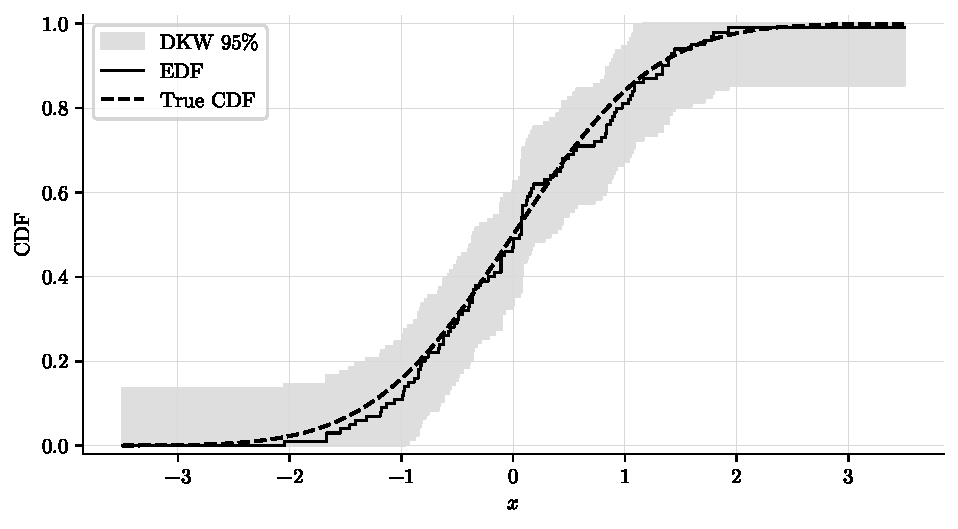
\includegraphics[width=.88\textwidth]{edf_dkw.pdf}
\caption{EDF và băng DKW 95\% trên một mẫu chuẩn mô phỏng, $n=100$.
Đường liền là CDF thật để đối chiếu; băng tính từ dữ liệu. Một hình
đơn lẻ không chứng minh mức bao phủ qua các mẫu lặp lại.}
\end{figure}
\intuition{Khoảng tại điểm là bảo đảm cho một ngưỡng; băng DKW là bảo đảm
cho toàn bộ đường. Cùng mức tin cậy, yêu cầu đồng thời thường cần băng rộng hơn.}
\pitfall{Lấy 100 khoảng Wald mức 95\% không tạo ra một băng đồng thời 95\%.
EDF có bước nhảy không làm DKW mất hiệu lực.}
\source{\cite{slide1}, slide 16--20; \cite{wasserman}, Chương 2}

\section{Functional và nguyên lý thế}
Một \emph{functional} là ánh xạ từ phân phối thành một số hoặc vectơ:
$T:F\mapsto T(F)$. Nguyên lý thế định nghĩa
\[
\boxed{\widehat\theta=T(\Fhat).}
\]
Nếu $T$ liên tục tại $F$ theo chuẩn sup của CDF thì Glivenko--Cantelli
và tính liên tục cho $T(\Fhat)\xrightarrow{a.s.}T(F)$.
Tính liên tục là giả thiết, không phải tính chất của mọi functional.
Chẳng hạn trung bình trên miền không bị chặn không liên tục theo chuẩn sup:
$F_m=(1-1/m)\delta_0+(1/m)\delta_{m^2}$ cách $\delta_0$ không quá
$1/m$ về CDF, nhưng trung bình của $F_m$ bằng $m$. Trung bình mẫu vẫn
nhất quán khi moment tuyệt đối bậc nhất hữu hạn, nhờ LLN.

\subsection{Functional tuyến tính}
Với $T(F)=\int a(x)\,dF(x)$ và $\E|a(X)|<\infty$,
\[
T(\Fhat)=\int a(x)\frac1n\sum_i\delta_{X_i}(dx)
=\frac1n\sum_ia(X_i).
\]
Tích phân theo khối lượng điểm $\delta_{X_i}$ bằng giá trị hàm tại $X_i$.
Từ LLN, ước lượng nhất quán; từ tuyến tính của kỳ vọng, không chệch.
Nếu $\Var(a(X))<\infty$,
\[
\Var(T(\Fhat))=\frac{\Var(a(X))}{n},\qquad
\sqrt n[T(\Fhat)-T(F)]\Rightarrow N(0,\Var(a(X))).
\]
Trung bình, moment thô và xác suất một tập cố định là những ví dụ.

\subsection{Trung bình, phương sai và độ lệch}
Đặt $\mu=\int x\,dF$, $\sigma^2=\int(x-\mu)^2\,dF$.
\[
\widehat\mu=\overline X,\qquad
\widehat\sigma^2_{\rm plug}=\frac1n\sum_i(X_i-\overline X)^2
=\overline{X^2}-\overline X^2.
\]
Functional phương sai phi tuyến vì $\mu$ cũng phụ thuộc $F$.
Từ $\E\overline{X^2}=\sigma^2+\mu^2$ và
$\E\overline X^2=\sigma^2/n+\mu^2$, suy ra
\[
\E\widehat\sigma^2_{\rm plug}=\frac{n-1}{n}\sigma^2.
\]
Ước lượng không chệch là $s^2=(n-1)^{-1}\sum_i(X_i-\overline X)^2$,
không phải đúng estimator plug-in của functional phương sai.
Cả hai nhất quán nếu $\E X^2<\infty$.

Skewness của phân phối có $\sigma>0$ và moment tuyệt đối bậc ba hữu hạn:
\[
\gamma_1(F)=\frac{\E(X-\mu)^3}{\sigma^3},\qquad
\widehat\gamma_1=\frac{n^{-1}\sum_i(X_i-\overline X)^3}
{[n^{-1}\sum_i(X_i-\overline X)^2]^{3/2}}.
\]
Nếu phương sai mẫu bằng 0, tỷ số không xác định. Các phiên bản hiệu chỉnh
skewness trong phần mềm có thể khác công thức plug-in này.
\begin{example}
Với $(1,2,4,5)$, $\overline X=3$, tổng bình phương độ lệch là 10.
Phương sai plug-in là $2.5$, $s^2=10/3$. Tổng lập phương độ lệch là
$-8-1+1+8=0$, nên skewness plug-in bằng 0.
\end{example}

\subsection{Tương quan và quantile}
Với mẫu cặp $(X_i,Y_i)$, dùng \emph{phân phối thực nghiệm đồng thời}.
Khi hai phương sai dương,
\[
\widehat\rho=
\frac{\sum_i(X_i-\overline X)(Y_i-\overline Y)}
{\sqrt{\sum_i(X_i-\overline X)^2\sum_i(Y_i-\overline Y)^2}}.
\]
Các hệ số $1/n$ triệt tiêu giữa tử và mẫu. Không thể khôi phục tương quan
chỉ từ hai CDF biên: cần cấu trúc phụ thuộc của các cặp.

Với $0<p<1$, quantile là nghịch đảo suy rộng:
\[
q_p=\inf\{x:F(x)\geq p\},\qquad
\widehat q_p=\inf\{x:\Fhat(x)\geq p\}=X_{(\lceil np\rceil)}.
\]
Đây là quy ước quantile dùng xuyên suốt tài liệu. Với mẫu bốn điểm trên,
$\widehat q_{0.5}=2$, khác trung vị nội suy $3$ thường dùng trong mô tả.
Nếu $F$ có quantile duy nhất và liên tục, tăng thực sự quanh $q_p$,
ước lượng quantile nhất quán. Nếu thêm $f(q_p)>0$ và $f$ liên tục gần đó,
biểu diễn tuyến tính tiệm cận là
\[
\widehat q_p-q_p=
-\frac{\Fhat(q_p)-p}{f(q_p)}+o_P(n^{-1/2}),
\quad
\sqrt n(\widehat q_p-q_p)\Rightarrow
N\left(0,\frac{p(1-p)}{f(q_p)^2}\right).
\]
Đây là kết quả được viện dẫn về quantile; trực giác đến từ
$F(q_p+t)\approx p+f(q_p)t$. Sai số theo chiều đứng của EDF được chia
cho độ dốc để đổi sang sai số theo chiều ngang. Mật độ nhỏ quanh quantile
làm sai số vị trí lớn.
\intuition{Plug-in biến một phân phối thực nghiệm thành thống kê quen thuộc.
Tính đúng đắn của suy luận phụ thuộc moment, tính liên tục và mẫu số của
functional, không chỉ phụ thuộc EDF hội tụ.}
\source{\cite{slide1}, slide 30--35; \cite{wasserman}, Chương 2}

\section{Kiểm định sự phù hợp}
Xét $H_0:F=F_0$ với $F_0$ \emph{liên tục, được chỉ định đầy đủ}.
Khi đó $U_i=F_0(X_i)$ i.i.d. đều trên $[0,1]$ dưới $H_0$.
Điều này giải thích tính không phụ thuộc phân phối của các thống kê sau.

\subsection{Kolmogorov--Smirnov}
\[
D_n=\sup_x|\Fhat(x)-F_0(x)|.
\]
Với $X_{(1)}\leq\cdots\leq X_{(n)}$, cần kiểm tra hai phía của mỗi
bước nhảy. Trong các khoảng không có dữ liệu, EDF hằng còn $F_0$ không
giảm; độ lệch lớn nhất đạt ở giới hạn hai đầu khoảng. Vì vậy
\begin{align*}
D_n^+&=\max_i\left\{\frac in-F_0(X_{(i)})\right\},\\
D_n^-&=\max_i\left\{F_0(X_{(i)})-\frac{i-1}n\right\},\qquad
\boxed{D_n=\max(D_n^+,D_n^-).}
\end{align*}
DKW cho kiểm định bảo thủ hữu hạn mẫu: bác bỏ khi
$D_n>\sqrt{\log(2/\alpha)/(2n)}$.
Với phân phối liên tục, giới hạn của $\sqrt nD_n$ là
$\sup_{0\leq t\leq1}|B(t)|$, với $B$ là cầu Brown.
\[
\Pp\big(\sup_t|B(t)|>z\big)
=2\sum_{k=1}^{\infty}(-1)^{k-1}e^{-2k^2z^2},\quad z>0.
\]
Đây là định lý giới hạn được viện dẫn. Mốc tiệm cận 95\% thường dùng
là $1.358/\sqrt n$; cần bảng hoặc thuật toán chính xác khi mẫu nhỏ.

\subsection{Cramér--von Mises}
CvM đo sai khác bình phương, tích phân theo $F_0$:
\[
W_n^2=n\int[\Fhat(x)-F_0(x)]^2\,dF_0(x)
=\frac1{12n}+\sum_{i=1}^n
\left[F_0(X_{(i)})-\frac{2i-1}{2n}\right]^2.
\]
Để thấy nguồn gốc công thức, đặt $u_i=F_0(X_{(i)})$, $u_0=0$,
$u_{n+1}=1$. CDF thực nghiệm trên $(u_i,u_{i+1})$ bằng $i/n$:
\[
W_n^2=n\sum_{i=0}^n\int_{u_i}^{u_{i+1}}(i/n-t)^2\,dt.
\]
Lấy nguyên hàm $t^3/3-(i/n)t^2+(i/n)^2t$ và thu gọn các đầu mút,
ta được $n/3+\sum_i[u_i^2-(2i-1)u_i/n]$.
Hoàn thành bình phương từng hạng và dùng
$\sum_i(2i-1)^2=n(4n^2-1)/3$ cho công thức trên.

\subsection{Anderson--Darling}
AD tăng trọng số ở hai đuôi:
\[
A_n^2=n\int\frac{[\Fhat(x)-F_0(x)]^2}
{F_0(x)[1-F_0(x)]}\,dF_0(x).
\]
Khi $0<u_i<1$, công thức tính là
\[
\boxed{A_n^2=-n-\frac1n\sum_{i=1}^n(2i-1)
\{\log u_i+\log(1-u_{n+1-i})\}.}
\]
Có thể kiểm tra bằng chia khoảng như CvM và phân tích
\[
\frac{(c-t)^2}{t(1-t)}
=\frac{c^2}{t}+\frac{(1-c)^2}{1-t}-1.
\]
Nguyên hàm là $c^2\log t-(1-c)^2\log(1-t)-t$.
Thế $c=i/n$ trên từng khoảng; hiệu hệ số ở một đầu mút cho các trọng số
$(2i-1)/n$. Ở khoảng sát 0 hoặc 1, hệ số đi với log phân kỳ bằng 0;
lấy giới hạn một phía để thu gọn. Nếu dữ liệu có $u_i=0$ hoặc 1,
AD có thể vô hạn: không tùy ý thay log 0 bằng 0.

\begin{center}
\begin{tabular}{lll}
\toprule Kiểm định & Đo sai khác & Nhấn mạnh\\\midrule
KS & Sai khác lớn nhất & Vị trí lệch nhiều nhất\\
CvM & Bình phương tích phân & Sai khác trên toàn miền\\
AD & Bình phương có trọng số & Hai đuôi\\\bottomrule
\end{tabular}
\end{center}
\intuition{KS nhìn điểm tệ nhất; CvM cộng sai khác; AD phóng đại sai khác
ở những vùng CDF gần 0 hoặc 1. Không có thống kê tốt nhất cho mọi đối thuyết.}
\pitfall{Nếu dùng mẫu để ước lượng $\mu,\sigma$ rồi kiểm định với
$N(\widehat\mu,\widehat\sigma^2)$, bảng KS chuẩn không còn đúng. Cần
hiệu chỉnh tương ứng hoặc bootstrap tham số có bước fit lại trong mỗi lần
lặp. Với $F_0$ rời rạc, phân phối null cũng khác. Không bác bỏ $H_0$
không có nghĩa chứng minh $H_0$ đúng.}
\source{\cite{slide1}, slide 36--46}

\section{Tự kiểm tra trước khi sang Chương 2}
Bạn cần tự làm được: viết EDF có dữ liệu trùng; phân biệt $F_n(x)$ và
$F_n(x-)$; chứng minh covariance bằng tích chỉ báo; suy ra băng DKW;
giải thích vì sao phương sai plug-in có mẫu số $n$; tính KS bằng cả
$D_n^+$ và $D_n^-$. Chương 6 có ba bài KS và một bài EDF/DKW để luyện.

\chapter{Ước lượng mật độ bằng histogram}\label{ch:hist}
\section{Đếm trong ô rồi chia cho độ rộng}
Giả sử trước hết $X_i\in[0,1]$, phân phối có mật độ $f$ trên miền này.
Chia thành $m$ ô bằng nhau, $h=1/m$:
\[
B_j=[(j-1)h,jh),\quad j<m,\qquad B_m=[(m-1)h,1].
\]
Quy ước ô trái đóng, phải mở, ngoại trừ ô cuối, đảm bảo mỗi quan sát được
đếm đúng một lần. Đặt
\[
N_j=\sum_i\1_{\{X_i\in B_j\}},\quad
p_j=\int_{B_j}f(u)\,du,\quad \widehat p_j=N_j/n.
\]
Histogram ước lượng mật độ là
\[
\boxed{\widehat f_{\rm hist}(x)=\frac{\widehat p_j}{h}
=\frac{N_j}{nh},\quad x\in B_j,}
\]
và bằng 0 ngoài $[0,1]$. $p_j/h$ là chiều cao trung bình thật trong ô;
$\widehat p_j/h$ mới là ước lượng từ mẫu.

\step{Kiểm tra là mật độ.}
Chiều cao không âm. Vì diện tích của ô $j$ là chiều cao nhân chiều rộng,
\[
\int\widehat f_{\rm hist}(x)\,dx
=\sum_{j=1}^m\frac{N_j}{nh}h
=\frac1n\sum_jN_j=1.
\]
Trên $[a,b]$, dùng $h=(b-a)/m$, trung điểm
$c_j=a+(j-1/2)h$. Nếu chuyển $U=(X-a)/(b-a)$ về $[0,1]$,
thì mật độ gốc phải là $\widehat f_X(x)=\widehat f_U((x-a)/(b-a))/(b-a)$.
Không thiếu hệ số Jacobian này.
\intuition{Chiều cao histogram là ``xác suất trong ô trên mỗi đơn vị độ dài''.
Biểu đồ số đếm chỉ có chiều cao $N_j$ chưa phải mật độ chuẩn hóa.}
\source{\cite{slide2}, slide 12; \cite{wasserman}, Mục 6.2}

\section{Kỳ vọng và phương sai chính xác}
Mỗi $N_j\sim\operatorname{Binomial}(n,p_j)$, dù các số đếm giữa ô khác
nhau không độc lập. Với $x\in B_j$,
\[
\E\widehat f_{\rm hist}(x)=\frac{p_j}{h},\qquad
\boxed{\Var\widehat f_{\rm hist}(x)=\frac{p_j(1-p_j)}{nh^2}.}
\]
Từ $\Var N_j=np_j(1-p_j)$, chỉ cần chia cho $(nh)^2$.
Kỳ vọng không phải $f(x)$ nói chung: estimator lấy trung bình mật độ
trong ô chứ không khôi phục biến thiên bên trong ô.

\section{Taylor và độ chệch tại một điểm}
Giả sử $f\in C^2([0,1])$, các đạo hàm được hiểu một phía ở biên.
Với $u,x\in B_j$ và $\norm{f''}_\infty<\infty$,
\[
f(u)=f(x)+f'(x)(u-x)+O((u-x)^2).
\]
Vì $|u-x|\leq h$, tích phân phần dư trên một ô có độ dài $h$ là $O(h^3)$.
Đặt $c_j=(j-1/2)h$:
\begin{align*}
p_j&=hf(x)+f'(x)\int_{(j-1)h}^{jh}(u-x)\,du+O(h^3)\\
&=hf(x)+hf'(x)(c_j-x)+O(h^3),
\end{align*}
vì trung bình của $u$ trên ô là $c_j$.
Chia cho $h$, rồi trừ $f(x)$, nhận
\[
\boxed{\Bias(\widehat f_{\rm hist}(x))
=f'(x)(c_j-x)+O(h^2)=O(h).}
\]
Tại đúng trung điểm $x=c_j$, số hạng bậc nhất mất. Taylor quanh $c_j$
còn cho $p_j/h-f(c_j)=h^2f''(c_j)/24+o(h^2)$.
Đây là cải thiện ở trung điểm, không phải bias $O(h^2)$ cho toàn histogram.

Thế $p_j=hf(x)+O(h^2)$ vào phương sai:
\[
\frac{p_j(1-p_j)}{nh^2}
=\frac{f(x)}{nh}+O(1/n).
\]
Nếu $f(x)>0$, số hạng chính là $f(x)/(nh)$; nếu $f(x)=0$, không thể
hiểu ký hiệu xấp xỉ theo tỷ số với số hạng chính bằng 0.
Khi $h\to0$, $nh\to\infty$, bias và variance cùng về 0, nên histogram
nhất quán theo MSE tại những điểm thỏa điều kiện trên.
\intuition{Ở ô có mật độ tăng, trung bình ô lớn hơn giá trị bên trái và
nhỏ hơn giá trị bên phải. Dấu chệch phụ thuộc vị trí của $x$ so với trung
điểm, không chỉ phụ thuộc độ dốc.}
\source{\cite{slide2}, slide 13--14; \cite{wasserman}, trang in 128--129,
phụ lục chứng minh trang in 140--142 (PDF 149--151)}

\section{Từ sai số tại điểm đến MISE}
\subsection{Tích phân bình phương chệch: nguồn gốc 1/12}
Trong ô $B_j$, có thể viết đều theo $x$:
$b(x)=f'(c_j)(c_j-x)+O(h^2)$.
Khi bình phương, hạng chéo được chặn bởi $O(h^3)$ tại điểm;
tích phân qua $m=1/h$ ô tổng độ dài 1 cho phần dư $O(h^3)$.
\begin{align*}
\int_0^1b(x)^2\,dx
&=\sum_j f'(c_j)^2\int_{B_j}(c_j-x)^2\,dx+O(h^3)\\
&=\sum_j f'(c_j)^2\int_{-h/2}^{h/2}t^2\,dt+O(h^3)\\
&=\frac{h^3}{12}\sum_j f'(c_j)^2+O(h^3)\\
&=\frac{h^2}{12}\int_0^1f'(x)^2\,dx+o(h^2).
\end{align*}
Ở bước hai, đặt $t=x-c_j$, $dx=dt$. Bước ba dùng
$[t^3/3]_{-h/2}^{h/2}=h^3/12$. Bước cuối dùng hội tụ tổng Riemann
$h\sum_j f'(c_j)^2\to\int_0^1f'^2$.

\subsection{Phương sai tích phân: công thức chính xác}
Phương sai là hằng trong mỗi ô, nên
\begin{align*}
\int_0^1\Var\widehat f_{\rm hist}(x)\,dx
&=\sum_jh\frac{p_j(1-p_j)}{nh^2}\\
&=\frac1{nh}\left(\sum_jp_j-\sum_jp_j^2\right)\\
&=\boxed{\frac1{nh}\left(1-\sum_jp_j^2\right)}.
\end{align*}
Với $f$ liên tục, $p_j=hf(\xi_j)$ cho một $\xi_j\in B_j$;
$\sum_jp_j^2/h=h\sum_j f(\xi_j)^2\to\int_0^1 f^2$.
Vậy phương sai tích phân bằng
\[
\frac1{nh}-\frac1n\int_0^1f(x)^2\,dx+o(1/n).
\]
Số hạng $-R(f)/n$ có bậc nhỏ hơn $1/(nh)$ khi $h\to0$;
nó không bằng 0 trong công thức chính xác.

\subsection{Băng thông và tốc độ tối ưu}
Đặt $A=\int_0^1f'^2>0$. Biểu thức tiệm cận chính là
\[
\AMISE_{\rm hist}(h)=\frac{A}{12}h^2+\frac1{nh}.
\]
Đạo hàm bằng $Ah/6-1/(nh^2)$, nên
\[
\boxed{h_*=(6/A)^{1/3}n^{-1/3},\qquad
\AMISE_{\rm hist}(h_*)=
\frac{6^{2/3}}4 A^{1/3}n^{-2/3}.}
\]
Để kiểm tra hệ số, tại nghiệm $1/(nh_*)=Ah_*^2/6$, bằng hai lần
phần bình phương chệch. Tổng bằng $Ah_*^2/4$.
Với $h=1/m$, chọn số nguyên $m$ gần $1/h_*$, so sánh hai ứng viên
lân cận. Nếu $A=0$, công thức suy biến: với mật độ đều trên miền biết
trước $[0,1]$, một ô duy nhất cho mật độ đúng bằng 1, rủi ro 0.

\begin{example}
Với $f(x)=2x$ trên $[0,1]$, $A=4$, nên
$h_*=(3/(2n))^{1/3}$. Nếu $n=96$, $h_*=1/4$, $m=4$.
Phần bình phương chệch chính là $1/48$, phương sai chính $1/24$,
tổng $1/16$. Đây là AMISE, không phải MISE chính xác.
\end{example}
\intuition{Ô rộng giảm dao động số đếm nhưng làm mất độ dốc bên trong ô.
Ở tối ưu, hai thành phần có cùng bậc theo $n$, nhưng không bằng nhau
về hằng số. Histogram đạt $n^{-2/3}$ dưới điều kiện đang xét.}
\source{\cite{slide2}, slide 15--16; \cite{wasserman}, Mục 6.2}

\section{Leave-one-out cross-validation}
Ta muốn chọn $h$ mà không biết $A$. Khai triển mất mát của một mẫu:
\[
\ISE(h)=\int\widehat f_h^2-2\int\widehat f_h f+R(f).
\]
Hạng $R(f)$ không phụ thuộc $h$, nên bỏ khi tối ưu.
Thay $\int\widehat f_h f$ bằng trung bình leave-one-out:
\[
\widehat J(h)=\int\widehat f_h^2(x)\,dx
-\frac2n\sum_i\widehat f_{(-i),h}(X_i).
\]
Giữ \emph{cùng phân hoạch} khi bỏ quan sát, chỉ đổi số đếm và mẫu số.
Nếu $X_i\in B_j$, $\widehat f_{(-i),h}(X_i)=(N_j-1)/((n-1)h)$.
Do đó
\begin{align*}
\int\widehat f_h^2&=\frac1{n^2h}\sum_jN_j^2,\\
\frac2n\sum_i\widehat f_{(-i),h}(X_i)
&=\frac2{n(n-1)h}\sum_jN_j(N_j-1)\\
&=\frac2{n(n-1)h}\left(\sum_jN_j^2-n\right).
\end{align*}
Trừ hai dòng, đổi $N_j^2=n^2\widehat p_j^2$:
\[
\boxed{\widehat J(h)=\frac2{(n-1)h}
-\frac{n+1}{(n-1)h}\sum_j\widehat p_j^2.}
\]
Với phân hoạch cố định, $\E\widehat f_{(-i),h}(x)=p_j/h=
\E\widehat f_{n,h}(x)$ trên ô $j$. Vì $X_i$ độc lập với mẫu bỏ $i$,
\[
\E\widehat f_{(-i),h}(X_i)
=\int\E\widehat f_{(-i),h}(x)f(x)\,dx
=\E\int\widehat f_{n,h}(x)f(x)\,dx.
\]
Suy ra $\E\widehat J(h)=\MISE_n(h)-R(f)$.
Phần bình phương đầu dùng estimator cỡ mẫu $n$; không tự thay tất cả
thành estimator cỡ mẫu $n-1$.

\begin{example}
Mẫu $(0.1,0.2,0.4,0.8)$, ứng viên $m=2,4$.
Với $m=2$, số đếm $(3,1)$ và $\sum\widehat p_j^2=10/16$:
\[
\widehat J(1/2)=\frac2{3/2}-\frac5{3/2}\frac{10}{16}=-\frac34.
\]
Với $m=4$, số đếm $(2,1,0,1)$ và $\sum\widehat p_j^2=6/16$:
\[
\widehat J(1/4)=\frac2{3/4}-\frac5{3/4}\frac6{16}=\frac16.
\]
Chọn $m=2$ trong hai ứng viên. Điểm CV âm là bình thường vì nó ước lượng
MISE trừ một hằng số dương.
\end{example}
\pitfall{Nếu dùng chính $X_i$ để đánh giá mật độ có chứa nó, quan sát tự
đóng góp vào mật độ và làm thiên lệch tiêu chuẩn. Nếu chọn gốc ô từ mẫu,
chứng minh không chệch cho phân hoạch cố định không còn áp dụng nguyên xi.}
\intuition{CV dùng một quan sát làm điểm đánh giá cho mô hình học từ
những quan sát còn lại. Mục tiêu là tối ưu rủi ro, không phải làm đường
cong trông đẹp nhất bằng mắt.}
\source{\cite{slide2}, slide 17; \cite{wasserman}, Mục 6.1--6.2}

\section{Bốn hạn chế cốt lõi}
\begin{enumerate}
\item \textbf{Không liên tục.} Đường mật độ nhảy ở ranh giới ô; không phù
hợp nếu muốn đạo hàm trơn hoặc vị trí đỉnh ổn định.
\item \textbf{Nhạy với gốc chia ô.} Dịch phân hoạch có thể làm một đỉnh
bị tách hoặc gộp dù dữ liệu và độ rộng ô không đổi.
\item \textbf{Khả năng tận dụng độ trơn hạn chế.} Với hàm có độ dốc,
bias thường $O(h)$, tốc độ MISE $n^{-2/3}$, chậm hơn KDE bậc hai
trong lớp mật độ đủ trơn và điều kiện biên phù hợp.
\item \textbf{Khó mở rộng theo số chiều.} Với ô lập phương cạnh $h$,
số ô tăng như $h^{-d}$, dữ liệu trong mỗi ô ít đi; phương sai có bậc
$1/(nh^d)$.
\end{enumerate}
\begin{figure}[htbp]
\centering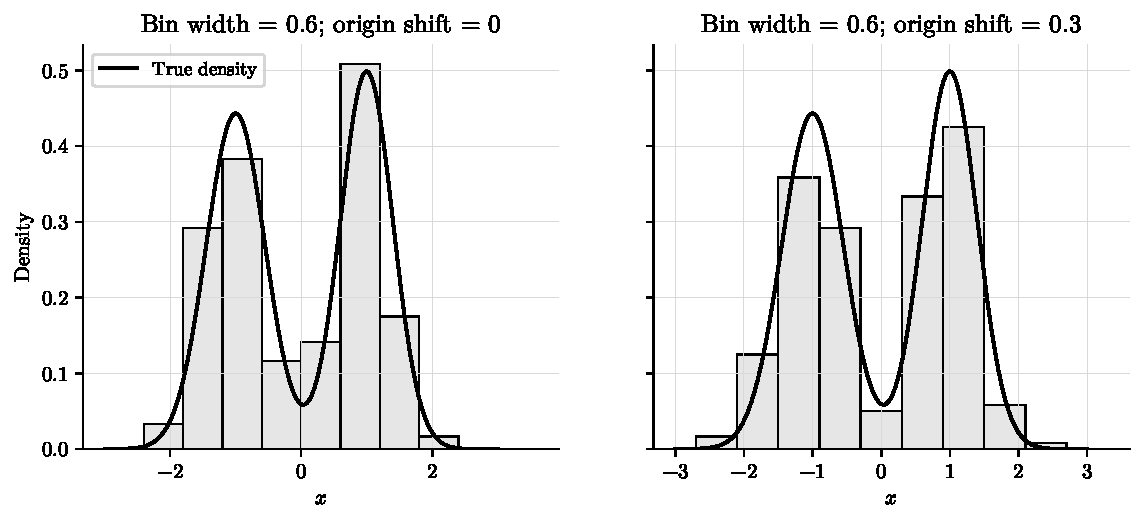
\includegraphics[width=.95\textwidth]{hist_origin.pdf}
\caption{Cùng mẫu và độ rộng ô, hai gốc chia ô khác nhau cho hai histogram.
Đường liền là mật độ hỗn hợp thật. Hình dùng ô trên toàn trục để minh họa
độ nhạy với gốc, khác thiết lập $h=1/m$ trên $[0,1]$ của phần chứng minh.}
\end{figure}
\intuition{KDE thay việc gán toàn bộ khối lượng vào một ô bằng việc đặt
một bản kernel quanh mỗi quan sát. Điều này loại bỏ gốc lưới cố định;
mức độ trơn vẫn phụ thuộc kernel được chọn.}
\source{\cite{slide2}, slide 18}

\chapter{Ước lượng mật độ bằng nhân}\label{ch:kde}
\section{Định nghĩa và tính hợp lệ}
Một kernel mật độ thông thường thỏa $K\geq0$, $\int_{\R} K=1$.
Trong các khai triển bậc hai, còn dùng $K$ đối xứng,
$\mu_2(K)=\int u^2K(u)\,du<\infty$ và $R(K)=\int K^2<\infty$.
Với $h>0$,
\[
\boxed{\fhat(x)=\frac1{nh}\sum_{i=1}^n
K\left(\frac{x-X_i}{h}\right).}
\]
Đây là trung bình của $n$ mật độ co giãn, mỗi mật độ có tâm $X_i$.
\begin{proof}[Kiểm tra chuẩn hóa]
Mỗi số hạng không âm, nên $\fhat\geq0$. Trong số hạng thứ $i$,
đặt $u=(x-X_i)/h$, $x=X_i+hu$, $dx=h\,du$:
\[
\int_{\R}\fhat(x)\,dx
=\frac1n\sum_i\int_{\R}\frac1hK((x-X_i)/h)\,dx
=\frac1n\sum_i\int_{\R} K(u)\,du=1.
\]
Tổng hữu hạn cho phép đổi tổng và tích phân. Nhân có phần âm vẫn cho
tích phân 1 nếu khả tích và chuẩn hóa, nhưng không đảm bảo không âm.
\end{proof}

\subsection{KDE liên hệ với EDF như thế nào?}
Đặt $G(t)=\int_{-\infty}^tK(u)\,du$. CDF của KDE là
\[
\widetilde F_{n,h}(x)=\frac1n\sum_iG((x-X_i)/h)
=\int K(u)\Fhat(x-hu)\,du.
\]
Đẳng thức thứ hai đến từ
$\1_{\{X_i\leq x-hu\}}=\1_{\{u\leq(x-X_i)/h\}}$.
Nếu $K$ liên tục, đạo hàm CDF này chính là KDE ở mọi điểm;
với Uniform, đẳng thức đạo hàm đúng hầu khắp nơi.
\intuition{EDF đặt các khối lượng điểm; KDE trải từng khối lượng đó ra
một vùng rộng theo $h$. Tăng $h$ là tăng mức trộn các vùng lân cận.}
\source{\cite{slide2}, slide 19--20; \cite{wasserman}, trang in 132 (PDF 141)}

\section{Bảy kernel và đạo hàm}
Trong bảng dưới, các kernel compact bằng 0 khi $|u|>1$.
Các biểu thức đạo hàm compact được ghi \emph{bên trong} $|u|<1$;
ngoài miền giá đỡ, các đạo hàm bằng 0. Các điểm nối phải kiểm tra riêng.
Đặt $t=|u|$, $\operatorname{sgn}(u)=u/|u|$ khi $u\ne0$.
\begin{longtable}{p{.18\textwidth}p{.74\textwidth}}
\toprule Kernel & $K(u)$, $K'(u)$, $K''(u)$\\\midrule\endhead
Gaussian & $K(u)=\varphi(u)=(2\pi)^{-1/2}e^{-u^2/2}$, $u\in\R$.
\newline $K'(u)=-u\varphi(u)$.
\newline $K''(u)=(u^2-1)\varphi(u)$.\\[5pt]
Epanechnikov & $K(u)=\frac34(1-u^2)$.
\newline $K'(u)=-\frac32u$.
\newline $K''(u)=-\frac32$.\\[5pt]
Uniform & $K(u)=\frac12$.
\newline $K'(u)=0$, $K''(u)=0$.\\[5pt]
Triangular & $K(u)=1-|u|$.
\newline $K'(u)=-\operatorname{sgn}(u)$ nếu $u\ne0$.
\newline $K''(u)=0$ nếu $u\ne0$.\\[5pt]
Biweight & $K(u)=\frac{15}{16}(1-u^2)^2$.
\newline $K'(u)=-\frac{15}{4}u(1-u^2)$.
\newline $K''(u)=\frac{15}{4}(3u^2-1)$.\\[5pt]
Triweight & $K(u)=\frac{35}{32}(1-u^2)^3$.
\newline $K'(u)=-\frac{105}{16}u(1-u^2)^2$.
\newline $K''(u)=-\frac{105}{16}(1-u^2)(1-5u^2)$.\\[5pt]
Tricube & $K(u)=\frac{70}{81}(1-t^3)^3$.
\newline $K'(u)=-\frac{70}{9}ut(1-t^3)^2$.
\newline $K''(u)=-\frac{140}{9}t(1-t^3)(1-4t^3)$.\\
\bottomrule
\end{longtable}
Quy ước $K(\pm1)=1/2$ cho Uniform; các kernel compact còn lại có
$K(\pm1)=0$. Giá trị tại hữu hạn điểm không ảnh hưởng moment nhưng có
thể ảnh hưởng bài tính điểm khi quan sát nằm đúng trên ranh giới.

\subsection{Khả vi tại điểm nối}
\begin{itemize}
\item Gaussian trơn mọi bậc.
\item Uniform không liên tục tại $u=\pm1$, nên không có đạo hàm cổ điển ở đó.
\item Epanechnikov liên tục nhưng không khả vi tại $\pm1$.
\item Triangular không khả vi tại $-1,0,1$.
\item Biweight khả vi liên tục bậc một; $K'(\pm1)=0$, nhưng $K''$
  không tồn tại tại $\pm1$ vì giới hạn độ dốc của $K'$ khác nhau.
\item Triweight khả vi liên tục bậc hai, $K'(\pm1)=K''(\pm1)=0$.
\item Tricube khả vi liên tục bậc hai tại cả $0$ và $\pm1$;
  $K'(0)=K''(0)=K'(\pm1)=K''(\pm1)=0$.
\end{itemize}
Ví dụ, Epanechnikov có đạo hàm từ phía trong tại $u=1$ bằng $-3/2$,
phía ngoài bằng 0. Viết ``$K'(1)=0$ do có chỉ báo'' là sai.
Với Tricube, tính bên $u>0$ rồi dùng tính chẵn của $K$, tính lẻ của
$K'$ để mở rộng; công thức $K''$ là chẵn và liên tục tại 0.

\subsection{Ước lượng đạo hàm mật độ}
Tại một điểm mà mọi số hạng có đạo hàm tương ứng,
\[
\boxed{\widehat f_h'(x)=\frac1{nh^2}\sum_iK'((x-X_i)/h),\qquad
\widehat f_h''(x)=\frac1{nh^3}\sum_iK''((x-X_i)/h).}
\]
Mỗi lần dùng quy tắc dây chuyền, $d[(x-X_i)/h]/dx=1/h$,
nên xuất hiện thêm một thừa số $1/h$.
Nếu một số hạng không khả vi, phải xét \emph{tổng} bằng giới hạn một
phía; các điểm gãy đôi khi có thể triệt tiêu. Không tự kết luận chỉ bằng
tính khả vi của một số hạng.

Đặc biệt, đạo hàm Uniform bằng 0 hầu khắp nơi, nhưng không phải một
ước lượng nhất quán hữu ích của $f'$ thông qua công thức đạo hàm cổ điển.
Đạo hàm theo nghĩa phân phối có khối lượng Dirac ở các bước nhảy;
nó không phải giá trị số của một hàm mật độ đạo hàm thông thường.
Với kernel đủ trơn, phương sai của estimator đạo hàm bậc $q$ có bậc
$1/(nh^{2q+1})$, cho thấy ước lượng đạo hàm khó hơn ước lượng mật độ.
\intuition{Độ trơn của KDE đến từ kernel. ``KDE luôn trơn'' không đúng
với Uniform hoặc Triangular. Muốn tìm độ cong một cách ổn định, nên
dùng kernel có đủ đạo hàm và bandwidth phù hợp với mục tiêu đạo hàm.}

\begin{figure}[htbp]
\centering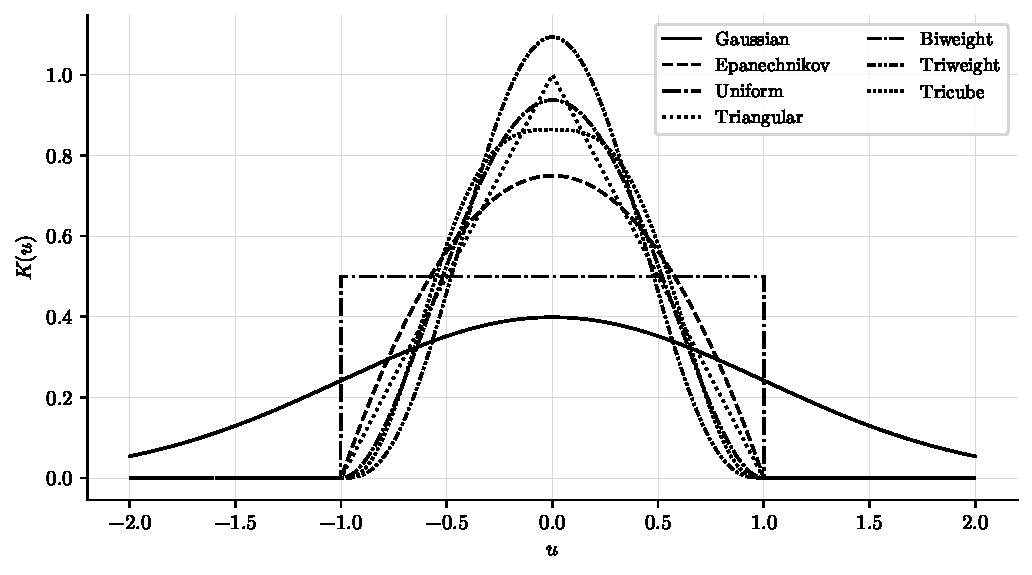
\includegraphics[width=.95\textwidth]{kernels.pdf}
\caption{Bảy kernel đã chuẩn hóa. Tất cả compact có giá đỡ $[-1,1]$;
Gaussian có đuôi trên toàn trục. Hình không thay thế kiểm tra khả vi tại điểm nối.}
\end{figure}

\section{Chứng minh độ chệch của KDE}
Xét điểm nội, hoặc mật độ đủ trơn trên toàn $\R$ mà không có gián đoạn
do biên. Một bộ giả thiết đủ cho khai triển dưới đây là $f\in C^4(\R)$
với đạo hàm bậc bốn bị chặn, $K$ đối xứng,
$\int|u|^4|K(u)|\,du<\infty$, $\int K=1$.
\step{Bước 1: đưa kỳ vọng về tích phân làm trơn.}
Đặt $Z_i(x)=h^{-1}K((x-X_i)/h)$. Tuyến tính cho
$\E\fhat(x)=\E Z_1(x)$. Dùng $u=(x-t)/h$,
\begin{align*}
\E\fhat(x)&=\int\frac1hK((x-t)/h)f(t)\,dt\\
&=\int K(u)f(x-hu)\,du.
\end{align*}
Hệ số $1/h$ triệt tiêu với $h$ trong vi phân; dấu âm của vi phân được
triệt tiêu khi đảo cận.

\step{Bước 2: Taylor đến bậc ba và chặn phần dư.}
\[
f(x-hu)=f(x)-hu f'(x)+\frac{h^2u^2}{2}f''(x)
-\frac{h^3u^3}{6}f'''(x)+\mathcal R_4(x,u,h),
\]
với $|\mathcal R_4|\leq\norm{f^{(4)}}_\infty h^4|u|^4/24$.
Tích phân phần dư nhân $K$ có trị tuyệt đối $O(h^4)$ nhờ moment
tuyệt đối bậc bốn hữu hạn.

\step{Bước 3: dùng moment của kernel.}
Vì kernel chẵn, $uK(u)$ và $u^3K(u)$ lẻ và khả tích, nên tích phân
trên miền đối xứng bằng 0. Vì $\int K=1$,
\begin{align*}
\E\fhat(x)&=f(x)+\frac{h^2}{2}\mu_2(K)f''(x)+O(h^4),\\
\boxed{\Bias(\fhat(x))}&\boxed{=\frac{h^2}{2}\mu_2(K)f''(x)+O(h^4).}
\end{align*}
Nếu chỉ có $f''$ liên tục và điều kiện chi phối phù hợp, kết quả thường
là $h^2\mu_2f''/2+o(h^2)$; không tự nâng phần dư lên $O(h^4)$.

\subsection{Ý nghĩa hình học của độ cong}
Với kernel không âm, $\mu_2(K)>0$. Ở đỉnh cong xuống,
$f''(x)<0$: chệch dẫn đầu âm, KDE trung bình làm thấp đỉnh
(undershoot). Ở đáy cong lên, $f''(x)>0$: chệch dẫn đầu dương,
KDE làm đầy đáy (overshoot). Nếu $f''(x)=0$, số hạng dẫn đầu mất;
cần xem bậc cao hơn thay vì dùng công thức tối ưu chia cho $f''(x)^2$.
\intuition{Làm trơn là lấy trung bình các giá trị lân cận. Đỉnh lấy trung
bình với các giá trị thấp hơn, đáy với các giá trị cao hơn. Độ cong,
không phải độ dốc đơn thuần, điều khiển bias bậc hai vì moment lẻ đã triệt tiêu.}
\source{\cite{slide2}, slide 21; \cite{wasserman}, trang in 133--134 (PDF 142--143)}

\section{Chứng minh phương sai và AMSE}
Giả sử thêm $f$ bị chặn và Lipschitz, $\int|u|K(u)^2\,du<\infty$.
\step{Bước 1: dùng độc lập giữa các quan sát.}
\[
\Var\fhat(x)=\frac1n\Var Z_1(x)
=\frac1n\{\E Z_1(x)^2-[\E Z_1(x)]^2\}.
\]
\step{Bước 2: tính moment bậc hai bằng đổi biến.}
\[
\E Z_1(x)^2=\int\frac1{h^2}K((x-t)/h)^2f(t)\,dt
=\frac1h\int K(u)^2f(x-hu)\,du.
\]
Do Lipschitz, $|f(x-hu)-f(x)|\leq C h|u|$, nên
\[
\E Z_1(x)^2=\frac{f(x)R(K)}h+O(1).
\]
Mặt khác, $\E Z_1(x)$ bị chặn bởi
$\norm f_\infty\int|K|$, nên bình phương kỳ vọng là $O(1)$.
Suy ra
\[
\boxed{\Var\fhat(x)=\frac{f(x)R(K)}{nh}+O(1/n).}
\]
Với $f$ chỉ liên tục tại $x$ và điều kiện chi phối, thường có dạng
$f(x)R(K)/(nh)+o(1/(nh))$; phần dư cụ thể cần điều kiện cụ thể.

\step{Bước 3: cộng bình phương chệch và phương sai.}
\[
\boxed{\AMSE_x(h)=\frac{h^4}{4}\mu_2(K)^2f''(x)^2
+\frac{f(x)R(K)}{nh}.}
\]
Nếu $f(x)>0$, $f''(x)\ne0$, tối ưu tại điểm cho
\[
h_{*,x}=\left[\frac{f(x)R(K)}{\mu_2(K)^2f''(x)^2}\right]^{1/5}n^{-1/5}.
\]
Nếu $h\to0$, $nh\to\infty$, bias và variance về 0,
nên $\fhat(x)\xrightarrow P f(x)$ qua bất đẳng thức Markov cho sai số
bình phương. Với kernel bị chặn, compact và $f$ liên tục tại $x$,
chứng minh nhất quán này không cần đủ bốn đạo hàm.
\intuition{Một cửa sổ rộng chứa khoảng $nhf(x)$ quan sát. Khi cửa sổ
hẹp đi, số quan sát hữu hiệu giảm và mật độ dao động mạnh hơn.}

\section{AMISE và băng thông toàn cục}
Để tích phân khai triển bias, cần kiểm soát phần dư theo chuẩn $L_2$,
không chỉ theo từng điểm. Một bộ giả thiết đủ là $f\in L_2(\R)$,
các đạo hàm yếu đến bậc bốn thuộc $L_2$, và
$\int|u|^4|K(u)|\,du<\infty$. Khi đó Taylor theo chuẩn $L_2$ cho
\[
\norm{\E\fhat-f-\tfrac12h^2\mu_2(K)f''}_2=O(h^4),
\]
nên tích phân bình phương bias bằng
$h^4\mu_2(K)^2R(f'')/4+O(h^6)$.
Hạng chéo được chặn bằng Cauchy--Schwarz:
$2\norm{h^2\mu_2f''/2}_2O(h^4)=O(h^6)$.

Phương sai tích phân có đẳng thức hữu ích, với $f_h=K_h*f$:
\begin{align*}
\int\Var\fhat(x)\,dx
&=\frac1{nh}\int\!\int K(u)^2 f(x-hu)\,du\,dx
-\frac1n\int f_h(x)^2\,dx\\
&=\boxed{\frac{R(K)}{nh}-\frac{R(f_h)}n}.
\end{align*}
Tích phân hai lớp đầu không âm nên dùng Tonelli; với mỗi $u$,
$\int f(x-hu)\,dx=1$. Nếu $K$ khả tích, $f\in L_2$ thì
$\norm{f_h}_2\leq\norm K_1\norm f_2$, nên số hạng trừ là $O(1/n)$.
Không được tích phân một chặn $O(1/n)$ hằng theo $x$ trên toàn $\R$
để kết luận nó vẫn là $O(1/n)$; đẳng thức này tránh lỗi đó.

Đặt $A=R(f'')>0$. Khi bỏ các hạng bậc nhỏ,
\[
\AMISE(h)=\frac{\mu_2(K)^2A}{4}h^4+\frac{R(K)}{nh}.
\]
Đạo hàm và giải:
\[
\mu_2(K)^2Ah^3-\frac{R(K)}{nh^2}=0,
\qquad
\boxed{h_* =\left[\frac{R(K)}{\mu_2(K)^2R(f'')}\right]^{1/5}n^{-1/5}.}
\]
Tại nghiệm, variance chính bằng bốn lần squared bias chính.
Vì vậy
\[
\boxed{\AMISE(h_*)=\frac54
R(K)^{4/5}\mu_2(K)^{2/5}R(f'')^{1/5}n^{-4/5}.}
\]
Histogram bậc một cho $n^{-2/3}$; KDE bậc hai cho $n^{-4/5}$
trong thiết lập đủ trơn, không bị chệch biên chi phối.
Đây là tốc độ MISE, không phải tốc độ RMSE: căn của $n^{-4/5}$
là $n^{-2/5}$.

\begin{figure}[htbp]
\centering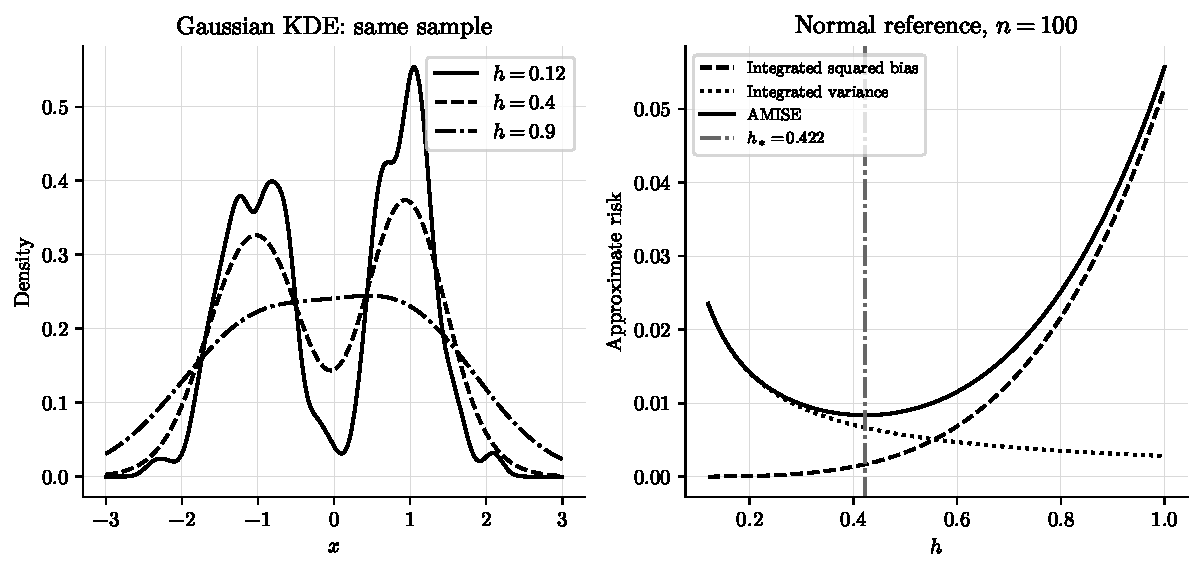
\includegraphics[width=.95\textwidth]{bandwidth_risk.pdf}
\caption{Trái: cùng mẫu, ba bandwidth KDE Gaussian. Phải: hai thành phần
AMISE và tổng của chúng trong mô hình chuẩn chuẩn tắc, $n=100$.
Các đường AMISE là xấp xỉ lý thuyết, không phải MISE thực nghiệm.}
\end{figure}
\intuition{Bandwidth nhỏ không miễn phí: giảm chệch nhưng tăng phương sai.
So sánh kernel cùng bậc thường thay đổi hằng số; thay bandwidth thay đổi
cả hai thành phần rủi ro theo các lũy thừa khác nhau.}
\source{\cite{slide2}, slide 25--26; \cite{wasserman}, trang in 133--135 (PDF 142--144)}

\section{Quy tắc tham chiếu chuẩn và Silverman}
\subsection{Dẫn ra hệ số 1.06}
Giả sử dùng kernel Gaussian và lấy mật độ chuẩn $N(\mu,\sigma^2)$ làm
tham chiếu. Với $z=(x-\mu)/\sigma$,
\[
f(x)=\frac1\sigma\varphi(z),\qquad
f''(x)=\frac{z^2-1}{\sigma^3}\varphi(z).
\]
Vì $dx=\sigma\,dz$,
\begin{align*}
R(f'')&=\frac1{2\pi\sigma^5}\int(z^2-1)^2e^{-z^2}\,dz\\
&=\frac1{2\pi\sigma^5}
\left(\frac{3\sqrt\pi}4-2\frac{\sqrt\pi}2+\sqrt\pi\right)
=\frac{3}{8\sqrt\pi\sigma^5}.
\end{align*}
Các tích phân được tính từ $\int e^{-z^2}=\sqrt\pi$ và tích phân từng
phần $\int z^{2k}e^{-z^2}=(2k-1)\int z^{2k-2}e^{-z^2}/2$.
Hạng biên $z^{2k-1}e^{-z^2}$ về 0 ở hai đầu.
Với Gaussian, $\mu_2(K)=1$, $R(K)=1/(2\sqrt\pi)$, nên
\[
h_*^5=\frac{1/(2\sqrt\pi)}{3/(8\sqrt\pi\sigma^5)n}
=\frac{4\sigma^5}{3n},\qquad
\boxed{h_{\rm NR}=(4/3)^{1/5}\sigma n^{-1/5}
\approx1.059224\sigma n^{-1/5}.}
\]
Thay $\sigma$ bằng độ lệch chuẩn mẫu $s$ cho $1.06s n^{-1/5}$.
Mô hình chuẩn là giả thiết dùng để tính bandwidth, không phải kết luận
rằng dữ liệu thật có phân phối chuẩn.

\subsection{Các phiên bản thực hành cần phân biệt}
Ở $N(\mu,\sigma^2)$, $\IQR=2\Phi^{-1}(0.75)\sigma\approx1.349\sigma$.
Đặt $a=\min\{s,\IQR/1.34\}$. Wasserman dùng $1.06a n^{-1/5}$
cho quy tắc tham chiếu chuẩn; quy tắc Silverman bền vững thường viết
$0.9a n^{-1/5}$. Hệ số $0.9$ không xuất phát từ cùng phép tối ưu chuẩn
vừa chứng minh.
Trong bài số của giáo trình, nếu không ghi khác, dùng
$s^2=(n-1)^{-1}\sum_i(X_i-\overline X)^2$ và hệ số chính xác
$(4/3)^{1/5}$, rồi mới làm tròn thành 1.06 khi cần minh họa.
Nếu tính IQR, dùng quantile thực nghiệm đã định nghĩa ở Chương 1;
các phần mềm nội suy có thể cho IQR khác ở mẫu nhỏ.
Nếu $s=0$, công thức cho bandwidth 0, không hợp lệ cho KDE:
phải có thông tin về độ phân giải hoặc chọn một bandwidth dương bên ngoài
quy tắc; không âm thầm chia cho 0.
\intuition{Quy tắc chuẩn nhanh vì thay đại lượng khó $R(f'')$ bằng công
thức của một mật độ tham chiếu. Mật độ nhiều đỉnh hoặc có đỉnh hẹp có thể
bị làm trơn quá mức; CV là một lựa chọn khác.}
\source{\cite{slide2}, slide 27; \cite{wasserman}, trang in 135 (PDF 144)}

\section{LOOCV cho KDE: công thức hữu hạn mẫu chính xác}
Giữ cùng $h$ khi bỏ quan sát:
\[
\widehat f_{(-i),h}(X_i)=\frac1{(n-1)h}
\sum_{j\ne i}K((X_i-X_j)/h).
\]
Với $n\geq2$, dùng
\[
\widehat J(h)=\int\fhat^2(x)\,dx
-\frac2n\sum_i\widehat f_{(-i),h}(X_i).
\]
Để tính tích phân đầu, khai triển bình phương thành tổng đôi. Trong cặp
$(i,j)$, đặt $u=(x-X_i)/h$, $dx=h\,du$:
\[
\int\frac1{h^2}K((x-X_i)/h)K((x-X_j)/h)\,dx
=\frac1h\int K(u)K(u+(X_i-X_j)/h)\,du.
\]
Đặt $C_K(v)=\int K(u)K(u+v)\,du$. Với kernel chẵn,
$C_K=K*K$ và ký hiệu $K^{(2)}$ thường được dùng.
Suy ra công thức chính xác
\[
\boxed{\widehat J(h)=\frac1{n^2h}\sum_{i,j}C_K((X_i-X_j)/h)
-\frac2{n(n-1)h}\sum_{i\ne j}K((X_i-X_j)/h).}
\]
Tổng đầu có đường chéo, tổng sau không có. Với Gaussian,
\[
C_K(v)=\frac1{2\sqrt\pi}e^{-v^2/4},
\]
là mật độ $N(0,2)$, có độ lệch chuẩn $\sqrt2$, không phải 2.
Với Uniform, $C_K(v)=(2-|v|)_+/4$, vì tích hai chiều cao bằng $1/4$
trên khoảng giao dài $(2-|v|)_+$.

\step{Tính không chệch của tiêu chuẩn.}
$X_i$ độc lập với mẫu bỏ $i$, nên
$\E\widehat f_{(-i),h}(X_i)=\int f_h(x)f(x)\,dx$.
Mặt khác $\E\fhat=f_h$ dù dùng $n$ hay $n-1$ quan sát.
Khai triển MISE cho
\[
\boxed{\E\widehat J(h)=\MISE_n(h)-R(f).}
\]
Điều kiện $f\in L_2$, $K\in L_1\cap L_2$ đảm bảo các hạng này hữu hạn.
Đẳng thức đúng cho $h$ cố định; chọn cực tiểu theo dữ liệu không làm
$\widehat J(\widehat h)$ thành ước lượng không chệch của rủi ro được chọn.

Trong thực hành, chọn một tập hữu hạn bandwidth dương và lấy điểm CV nhỏ
nhất; nếu bằng nhau, quy ước chọn bandwidth lớn hơn để ưu tiên làm trơn.
Một ứng viên nhỏ nhất ở mép lưới là tín hiệu cần kiểm tra phạm vi lưới.
Không có bảo đảm rằng CV hữu hạn mẫu luôn chọn tốt nhất; với dữ liệu
trùng lặp, bandwidth cực nhỏ có thể gây hành vi suy biến.
\intuition{LOO loại sự tự đóng góp $K(0)/(nh)$ của mỗi điểm. Tổng đôi
chính xác giúp tính CV mà không cần tích phân số cả một đường KDE.}
\source{\cite{wasserman}, trang in 135--136 (PDF 144--145), phương trình 6.33;
ở đây giữ mẫu số $n-1$ chính xác thay vì dùng dạng xấp xỉ 6.35}

\section{Nhân bậc cao}
Trong tài liệu này, kernel bậc $\ell$ nghĩa là
\[
\int K=1,\quad\mu_j(K)=0\ (1\leq j<\ell),\quad\mu_\ell(K)\ne0.
\]
Đây là một quy ước; Tsybakov dùng cách đặt tên khác cho số moment bị
triệt tiêu. Luôn kiểm tra các moment thực tế thay vì chỉ đọc chữ ``bậc''.
Với $f$ có đủ đạo hàm, moment tuyệt đối bậc $\ell$ hữu hạn và điều kiện
phần dư thích hợp,
\[
\Bias(\fhat(x))=
\frac{(-h)^\ell}{\ell!}\mu_\ell(K)f^{(\ell)}(x)+o(h^\ell).
\]
Tất cả hạng bậc thấp mất nhờ moment bằng 0.
Nếu khai triển đúng theo $L_2$, MISE có phần chính
$Ah^{2\ell}+R(K)/(nh)$, nên
\[
h_*\asymp n^{-1/(2\ell+1)},\qquad
\MISE=O(n^{-2\ell/(2\ell+1)}).
\]
Không thể dùng tốc độ này khi mật độ không có độ trơn tương ứng.

\begin{example}[Kernel Gaussian bậc bốn]
Đặt $K_4(u)=(3-u^2)\varphi(u)/2$.
Moment chuẩn tắc cho $\E Z^2=1$, $\E Z^4=3$, $\E Z^6=15$:
\[
\int K_4=(3-1)/2=1,\quad
\mu_2(K_4)=(3-3)/2=0,\quad
\mu_4(K_4)=(9-15)/2=-3.
\]
Moment lẻ bằng 0 do đối xứng. Vậy đây là kernel bậc bốn theo quy ước
trên, cho bias $-h^4f^{(4)}(x)/8+o(h^4)$ và tốc độ $n^{-8/9}$.
Nhưng $K_4(u)<0$ khi $|u|>\sqrt3$: KDE có thể âm.
\end{example}
Một kernel không âm, chuẩn hóa không thể có $\mu_2=0$ trừ một phân
phối tập trung tại 0, vốn không phải kernel mật độ thông thường:
$u^2K(u)\geq0$ mà tích phân bằng 0 thì $K=0$ hầu khắp nơi ngoài 0.
Do đó triệt tiêu moment bậc hai buộc kernel thông thường có phần âm.
\intuition{Nhân bậc cao dùng các vùng âm để bù chệch của vùng dương.
Đổi lại tốc độ nhanh hơn trên hàm rất trơn là mất tính không âm và
tăng yêu cầu về độ trơn của mật độ.}
\source{\cite{slide2}, slide 22; \cite{tsybakov}, Mục 1.2.2}

\section{Lớp Hölder và chặn rủi ro}
\subsection{Định nghĩa không suy biến ở bậc nguyên}
Với $\beta>0$, đặt $r=\lceil\beta\rceil-1$, $\eta=\beta-r\in(0,1]$.
Một hàm trong $\Sigma(\beta,L)$ có đạo hàm liên tục đến bậc $r$ và
\[
|f^{(r)}(x)-f^{(r)}(y)|\leq L|x-y|^\eta.
\]
Đồng thời yêu cầu $f\geq0$, $\int f=1$ khi xét lớp mật độ;
dùng thêm chặn $\norm f_\infty\leq M$ khi chứng minh chặn phương sai.
Với $r=0$ đây là điều kiện trực tiếp trên $f$; với $\beta=2$, $f'$ là
Lipschitz. Không viết $|f(x)-f(y)|\leq L|x-y|^\beta$ cho mọi
$\beta>1$ trên một khoảng: điều kiện ấy buộc $f$ hằng.

\subsection{Chặn bias bằng Taylor có phần dư Hölder}
Taylor đến bậc $r$ cho
\[
f(x+t)=\sum_{j=0}^r\frac{f^{(j)}(x)}{j!}t^j+\mathcal R_\beta,
\qquad |\mathcal R_\beta|\leq\frac{L}{r!}|t|^\beta.
\]
Với $r=0$ đây chính là định nghĩa. Với $r\geq1$, Taylor dạng tích phân
đến bậc $r-1$, rồi trừ và cộng $f^{(r)}(x)$ trong tích phân:
\[
\mathcal R_\beta=
\frac{t^r}{(r-1)!}\int_0^1(1-s)^{r-1}
[f^{(r)}(x+st)-f^{(r)}(x)]\,ds.
\]
Trị tuyệt đối bị chặn bởi $L|t|^{r+\eta}/(r-1)!$ nhân
$\int_0^1(1-s)^{r-1}s^\eta ds\leq1/r$; đó là chặn đã nêu.
Nếu kernel triệt tiêu moment $1,\ldots,r$ và
$M_\beta(K)=\int|u|^\beta|K(u)|\,du<\infty$, thì
\begin{align*}
\Bias(\fhat(x))&=\int K(u)\mathcal R_\beta(x,-hu)\,du,\\
\boxed{|\Bias(\fhat(x))|}&\boxed{\leq (L/r!)M_\beta(K)h^\beta.}
\end{align*}
Tính đối xứng chỉ tự triệt tiêu moment lẻ, không triệt tiêu mọi moment.

\subsection{Chặn variance và MSE}
Không cần Taylor để có chặn phương sai:
\[
\Var\fhat(x)\leq\frac1n\E Z_1(x)^2
=\frac1{nh}\int K^2(u)f(x-hu)\,du
\leq\boxed{\frac{MR(K)}{nh}}.
\]
Đặt $C_b=(L/r!)M_\beta(K)$, ta có
\[
\sup_f\MSE_f(\fhat(x))\leq C_b^2h^{2\beta}+\frac{MR(K)}{nh}.
\]
Chọn $h\asymp n^{-1/(2\beta+1)}$ cho chặn
$O(n^{-2\beta/(2\beta+1)})$. Đây là chặn đều \emph{tại điểm}; không
tích phân hằng số trên toàn $\R$ để suy ra MISE hữu hạn.
Để có MISE cùng bậc, dùng điều kiện độ trơn theo chuẩn $L_2$ như lớp
Sobolev, hoặc miền compact với xử lý biên và chặn bias đồng đều.
Phương sai tích phân luôn bị chặn bởi $R(K)/(nh)$.
\source{\cite{tsybakov}, Mệnh đề 1.1--1.2 và Định lý 1.1,
trang in 4--9 (PDF 15--20); Mệnh đề 1.4, trang in 12 (PDF 23)}

\subsection{Minimax: vì sao đây là tốc độ tốt nhất?}
Với lớp mật độ Hölder có chặn nêu trên và $x_0$ ở miền nội thích hợp,
đặt
\[
\mathcal R_n^*(x_0)=\inf_{T_n}\sup_{f\in\mathcal F}
\E_f[T_n-f(x_0)]^2.
\]
Infimum chạy trên mọi estimator đo được từ mẫu. Kết quả lower bound
cho lớp đủ phong phú là
\[
\mathcal R_n^*(x_0)\geq c n^{-2\beta/(2\beta+1)},
\]
với $c>0$ phụ thuộc lớp, không phụ thuộc $n$. Kết hợp chặn trên vừa chứng
minh cho tốc độ minimax. Chặn trên của riêng KDE không tự chứng minh
lower bound cho mọi estimator.

\step{Phác thảo lower bound tại điểm.}
Chọn mật độ nền $f_0$ dương quanh $x_0$, thêm một nhiễu
$\delta a^\beta\psi((x-x_0)/a)$ có $\int\psi=0$, $\psi(0)\ne0$,
compact và đủ trơn. Với $\delta$ nhỏ, mật độ mới $f_1$ vẫn không âm,
chuẩn hóa và ở cùng lớp. Hai giá trị tại $x_0$ cách nhau bậc $a^\beta$.
\[
\int\frac{(f_1-f_0)^2}{f_0}\,dx=O(a^{2\beta+1}),
\quad
\operatorname{KL}(P_1^n,P_0^n)=O(na^{2\beta+1}).
\]
Chọn $a\asymp n^{-1/(2\beta+1)}$ để hai luật mẫu khó phân biệt.
Lower bound kiểm định hai giả thuyết (Le Cam) buộc sai số bình phương
ít nhất có bậc $a^{2\beta}$. Đây là phác thảo, các bổ đề kiểm định được
viện dẫn từ \cite{tsybakov}, Chương 2.
Với rủi ro tích phân, đặt nhiều nhiễu trên các ô rời nhau và dùng
Assouad/Fano; Wasserman Định lý 6.31 cho lower bound MISE trên lớp
$R(f^{(m)})\leq c^2$, đạt $n^{-2m/(2m+1)}$.
\intuition{Độ trơn cho phép mượn thông tin ở lân cận. Lower bound nói
rằng dù chọn thuật toán nào, một lớp có nhiều nhiễu nhỏ khó phân biệt
vẫn đặt ra giới hạn thông tin. Minimax là kết luận theo lớp và loại mất mát.}

\section{Chệch biên và cách xử lý}
Giả sử miền giá đỡ là $[0,\infty)$, $f(0+)>0$, kernel chẵn. Tại 0,
\[
\E\fhat(0)=\int_0^\infty\frac1hK(-t/h)f(t)\,dt
=\int_0^\infty K(u)f(hu)\,du.
\]
Nếu $f$ liên tục phải và điều kiện chi phối thỏa,
giới hạn bằng $f(0+)\int_0^\infty K=f(0+)/2$. Vì vậy
\[
\boxed{\Bias(\fhat(0))\to-f(0+)/2.}
\]
Chệch ngay tại biên có thể là $O(1)$, không phải $O(h)$.
Vùng biên rộng $O(h)$ với chệch không tiêu biến có thể làm squared bias
tích phân bậc $O(h)$ và phá tốc độ AMISE nội miền.

\subsection{Phản xạ}
Trên nửa trục, định nghĩa
\[
\widehat f_R(x)=\frac1{nh}\sum_i
\{K((x-X_i)/h)+K((x+X_i)/h)\},\quad x\geq0.
\]
Với kernel chẵn, tổng diện tích của hai bản kernel trên $[0,\infty)$
bằng 1 cho mỗi quan sát: phần bị cắt của bản tâm $X_i$ được bản tâm
$-X_i$ bù lại. Vì vậy estimator không âm và tích phân 1 trên nửa trục.
Tại 0,
\begin{align*}
\E\widehat f_R(0)
&=2\int_0^\infty K(u)f(hu)\,du\\
&=f(0+)+2hf'(0+)\int_0^\infty uK(u)\,du+O(h^2).
\end{align*}
Phản xạ bỏ chệch hằng số, nhưng nếu $f'(0+)\ne0$, bias vẫn $O(h)$.
Nếu $f'(0+)=0$ và đủ trơn, có thể đạt $O(h^2)$.
Với $f(x)=e^{-x}\1_{x\geq0}$ và Uniform,
$\E\fhat(0)=(1-e^{-h})/(2h)$,
$\E\widehat f_R(0)=(1-e^{-h})/h=1-h/2+O(h^2)$.

\subsection{Boundary kernel}
Ở biên 0, có thể dùng trọng số tương đương $L$ trên $[0,1]$ thỏa
$\int_0^1L=1$, $\int_0^1uL(u)du=0$. Ví dụ $L(u)=4-6u$ trên
$[0,1]$. Khi đó estimator
$(nh)^{-1}\sum_i L(X_i/h)\1_{\{0\leq X_i\leq h\}}$
có kỳ vọng $\int_0^1L(u)f(hu)du=f(0)+O(h^2)$.
Moment bậc một triệt tiêu cả khi cửa sổ chỉ một phía.
Nhưng $L$ có phần âm; estimator không tự động là mật độ không âm,
và đây là công thức \emph{tại biên}, không phải kernel chung cho toàn miền.
Chỉ chuẩn hóa lại kernel bị cắt mà không triệt tiêu moment bậc một
thường chỉ cải thiện bias về $O(h)$.

\begin{figure}[htbp]
\centering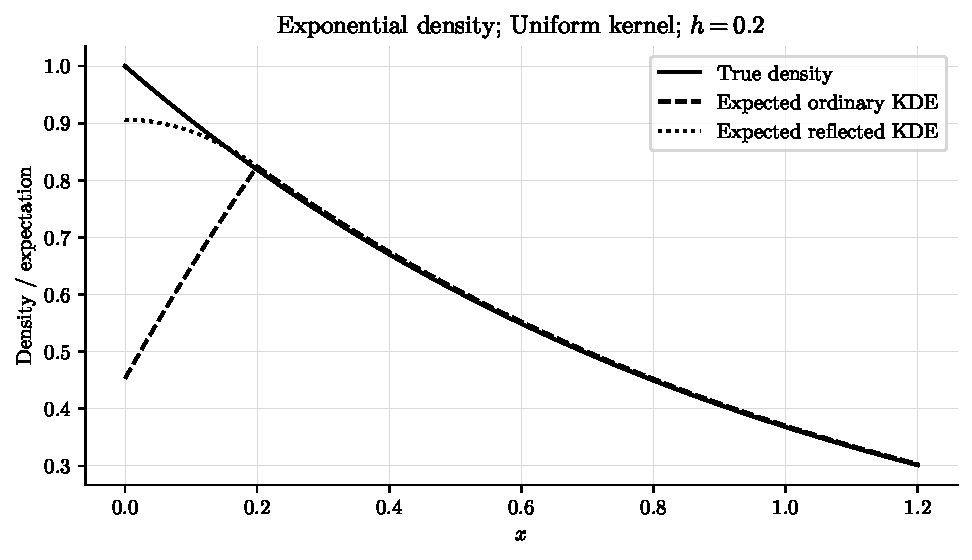
\includegraphics[width=.9\textwidth]{boundary.pdf}
\caption{Mật độ mũ và kỳ vọng KDE Uniform tại $h=0.2$.
Reflection sửa phần thiếu khối lượng nhưng vẫn còn chệch bậc nhất tại 0.
Đường vẽ là kỳ vọng tính giải tích, không phải KDE của một mẫu.}
\end{figure}
\intuition{Kernel đối xứng chỉ triệt tiêu moment lẻ khi có dữ liệu ở cả
hai phía. Ở biên, một phía không tồn tại nên phép triệt tiêu mất hiệu lực.}

\section{Suy luận thống kê cho mật độ: kiểm soát chệch}
Ở điểm nội với $f(x)>0$, kernel và mật độ thỏa điều kiện CLT cho mảng
tam giác, $h\to0$, $nh\to\infty$,
\[
\sqrt{nh}[\fhat(x)-\E\fhat(x)]\Rightarrow N(0,f(x)R(K)).
\]
CLT này canh tâm ở $f_h(x)=\E\fhat(x)$, không tự ở $f(x)$.
Nếu $h\asymp n^{-1/5}$, bias $h^2$ và độ lệch chuẩn $(nh)^{-1/2}$
cùng bậc. Muốn bỏ bias để suy luận cho $f(x)$, một điều kiện đủ là
\[
\sqrt{nh}\,h^2\to0\quad\Longleftrightarrow\quad nh^5\to0,
\]
đồng thời $nh\to\infty$; đây là undersmoothing.
Khi các điều kiện này thỏa, khoảng tại điểm xấp xỉ là
$\fhat(x)\pm z_{1-\alpha/2}\sqrt{R(K)\fhat(x)/(nh)}$ với kernel
mật độ không âm. Một băng đồng thời cần thêm kiểm soát supremum của
quá trình ngẫu nhiên, không chỉ lấy cùng hệ số chuẩn ở mọi $x$.
\intuition{Bandwidth tối ưu để ước lượng theo MSE chưa chắc phù hợp để
lập khoảng tin cậy bỏ qua bias. Chương 5 tiếp tục vấn đề này với Root--Unroot.}
\source{\cite{slide2}, slide 28; \cite{wasserman}, Chương 5, Mục 5.7 và Chương 6}

\chapter{Ước lượng chiếu và lựa chọn mô hình}\label{ch:projection}
\section{Bắt đầu bằng ba câu hỏi, chưa cần toán cao cấp}
Bạn đã gặp histogram ở Chương 2: chia miền thành các ô, đếm dữ liệu,
rồi vẽ một chiều cao trên mỗi ô. Ước lượng chiếu mở rộng ý tưởng này:
\emph{chọn một số hình dạng đơn giản, rồi ghép chúng thành đường ước lượng}.

Trong chương này, ta trả lời lần lượt ba câu hỏi:
\begin{enumerate}
\item \textbf{Ghép bằng cái gì?} Dùng các hàm cơ sở: có thể là hình chữ
nhật, hoặc sóng sin và cos.
\item \textbf{Mỗi hình dạng đóng góp bao nhiêu?} Tính các hệ số từ dữ liệu.
\item \textbf{Dùng bao nhiêu hình dạng?} Chọn số chiều $D$: ít quá thì
mất chi tiết, nhiều quá thì giữ cả nhiễu của mẫu.
\end{enumerate}
\textbf{Cách đọc.} Lần đầu, đọc từ ví dụ histogram đến phần oracle và câu
hỏi tự kiểm tra. Phần ``Đọc thêm'' ở cuối giữ các chứng minh nâng cao;
bạn có thể quay lại sau khi giải thích được ví dụ bằng lời.
Không cần hiểu chuỗi vô hạn ngay để tính được một ước lượng chiếu.

\intuition{Hãy coi $D$ là số thành phần bạn cho phép đường ước lượng sử
 dụng. Bài toán có hai bước riêng: với $D$ đã cho, dựng đường; sau đó mới
 so sánh các $D$ để chọn đường phù hợp.}

\section{Một ví dụ histogram dùng xuyên suốt chương}
\subsection{Dữ liệu và ba cách chia ô}
Giả sử dữ liệu nằm trên $[0,1]$. Cho tám quan sát
\[
X=(0.10,0.12,0.20,0.30,0.40,0.60,0.80,0.90),\qquad n=8.
\]
Ta thử $D=1,2,4$ ô bằng nhau. Độ rộng mỗi ô là $h=1/D$.
Chiều cao mật độ trong một ô luôn là
\[
\boxed{\text{chiều cao}=\frac{\text{số điểm trong ô}}{n\times h}.}
\]
\begin{center}
\begin{tabular}{cccc}
\toprule Số ô $D$ & Độ rộng $h$ & Số đếm trong các ô & Chiều cao mật độ\\\midrule
1 & $1$ & $(8)$ & $(1)$\\
2 & $1/2$ & $(5,3)$ & $(5/4,3/4)$\\
4 & $1/4$ & $(3,2,1,2)$ & $(3/2,1,1/2,1)$\\\bottomrule
\end{tabular}
\end{center}
Ví dụ, với $D=2$, ô trái có năm điểm nên chiều cao là
$5/(8\times1/2)=5/4$. Ô phải có ba điểm nên chiều cao là $3/4$.
Diện tích hai ô là $5/4\times1/2+3/4\times1/2=1$.

\subsection{Tại sao đây đã là một bài toán chọn mô hình?}
Với một ô, đường chỉ có một mức cao nên không thể hiện sự khác nhau giữa
hai nửa miền. Với bốn ô, đường có thể hiện nhiều chi tiết hơn; nhưng chỉ
một điểm đi sang ô kế bên cũng có thể làm chiều cao đổi đáng kể.
Cả ba đường đều được dựng từ cùng tám điểm. \emph{Nhiều ô hơn không tự
động có nghĩa gần mật độ thật hơn.} Ta chưa biết mật độ thật để chấm sai
số trực tiếp; đó là lý do cần tiêu chuẩn lựa chọn mô hình.

\begin{figure}[htbp]
\centering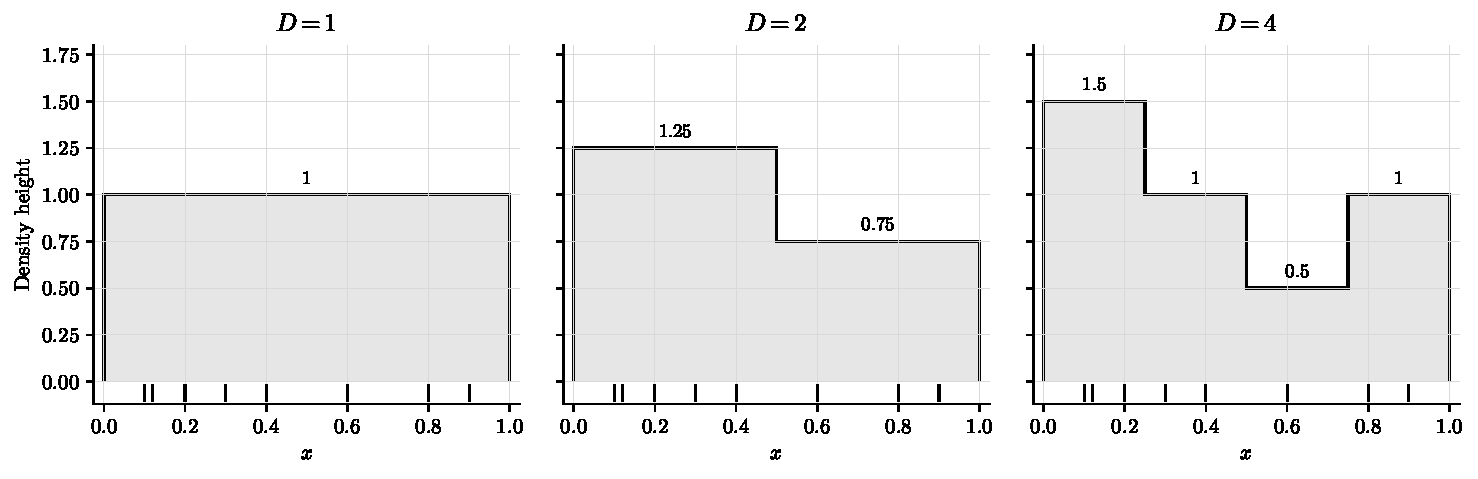
\includegraphics[width=.97\textwidth]{projection_models.pdf}
\caption{Cùng tám quan sát, ba mô hình histogram với $D=1,2,4$.
Các vạch dưới trục là dữ liệu. Chiều cao từng ô được tính trong bảng;
không có đường mật độ thật trong hình vì ví dụ chỉ cho dữ liệu.}
\end{figure}
\intuition{Ở ví dụ hàm bước, ``mô hình $D$ chiều'' chỉ là tập các đường
có một chiều cao trên mỗi ô. Chọn mô hình nghĩa là chọn mức độ chi tiết.}

\section{Hàm cơ sở và hệ số: đọc như một công thức ghép hình}
\subsection{Trước tiên, dùng hai hình chữ nhật}
Với $D=2$, đặt $B_1=[0,1/2)$, $B_2=[1/2,1]$.
Một hàm chỉ báo $\1_{B_j}(x)$ bằng 1 khi $x$ trong ô $j$, bằng 0 ở ngoài.
Ta có thể viết histogram thành
\[
\widehat f_2(x)=\frac54\1_{B_1}(x)+\frac34\1_{B_2}(x).
\]
Dòng này chỉ nói: ở ô trái, lấy chiều cao $5/4$; ở ô phải, lấy $3/4$.
Các hình chữ nhật là \emph{hàm cơ sở}; các số đứng trước chúng là
\emph{hệ số}. Với cơ sở tổng quát, hệ số không nhất thiết là chiều cao
hay xác suất của một ô.

\subsection{Tại sao trong slide lại có căn bậc hai?}
Để phép tính gọn hơn, ta dùng các hàm cơ sở được chuẩn hóa:
\[
\phi_1(x)=\sqrt2\,\1_{B_1}(x),\qquad
\phi_2(x)=\sqrt2\,\1_{B_2}(x).
\]
Mỗi hình chữ nhật cao $\sqrt2$, rộng $1/2$. Vì vậy tích phân
\emph{bình phương} của mỗi hàm bằng
$(\sqrt2)^2\times1/2=1$.
Hai hàm không chồng lên nhau, nên tích của chúng bằng 0 tại mọi điểm.
Ta gọi hai tính chất này là \emph{trực chuẩn}:
\[
\int_0^1\phi_1^2=\int_0^1\phi_2^2=1,\qquad
\int_0^1\phi_1\phi_2=0.
\]
``Chuẩn'' nghĩa là độ lớn đã đưa về 1; ``trực'' nghĩa là hai hình dạng
không có phần tích chung khi lấy tích phân. Với sin và cos, các hàm có
thể chồng lên nhau nhưng các phần dương và âm của tích triệt tiêu.

\subsection{Tính hệ số từ mẫu, rồi ghép lại}
Công thức hệ số mẫu là trung bình các giá trị hàm cơ sở tại dữ liệu:
\[
\widehat a_j=\frac1n\sum_{i=1}^n\phi_j(X_i).
\]
Ở ví dụ hai ô, $\phi_1(X_i)$ bằng $\sqrt2$ ở năm điểm, bằng 0 ở ba
điểm. Do đó
\[
\widehat a_1=\frac{5\sqrt2}{8},\qquad
\widehat a_2=\frac{3\sqrt2}{8}.
\]
Ghép hai hình dạng:
\begin{align*}
\widehat f_2(x)
&=\widehat a_1\phi_1(x)+\widehat a_2\phi_2(x)\\
&=\frac{5\sqrt2}{8}\sqrt2\,\1_{B_1}(x)
 +\frac{3\sqrt2}{8}\sqrt2\,\1_{B_2}(x)\\
&=\frac54\1_{B_1}(x)+\frac34\1_{B_2}(x).
\end{align*}
Hai căn nhân nhau thành 2, nên kết quả trùng histogram ban đầu.
\textbf{Bạn chưa học một estimator khác: bạn vừa viết lại histogram
bằng ngôn ngữ hàm cơ sở.}

Với $D$ ô, mỗi ô rộng $1/D$, cơ sở chuẩn hóa cao $\sqrt D$:
\[
\phi_{D,j}=\sqrt D\,\1_{B_j},\qquad
\widehat a_{D,j}=\frac{\sqrt D N_j}{n},\qquad
\widehat f_D(x)=\frac{DN_j}{n}\quad(x\in B_j).
\]
Chỉ số $D,j$ nhắc rằng cơ sở hàm bước thay đổi khi đổi phân hoạch.
\intuition{Hàm cơ sở cho hình dạng; hệ số cho mức đóng góp. Căn bậc hai
là cách chuẩn hóa để phép tính bình phương đơn giản, không phải một thao
 tác bí ẩn trên dữ liệu.}
\source{\cite{projection}, slide 8--12; \cite{slide2}, slide 30--31}

\section{Phân biệt ba đường: thật, xấp xỉ và ước lượng}
Đây là ba ký hiệu dễ nhầm nhất trong chương:
\begin{center}
\begin{tabular}{p{.12\textwidth}p{.39\textwidth}p{.37\textwidth}}
\toprule Ký hiệu & Đọc bằng lời & Ta có tính từ dữ liệu không?\\\midrule
$f$ & Mật độ thật cần tìm & Không, nói chung chưa biết.\\[3pt]
$f_D$ & Đường gần $f$ nhất trong mô hình $D$ đã chọn & Không, cần biết $f$.\\[3pt]
$\widehat f_D$ & Đường ta dựng từ mẫu, trong mô hình $D$ & Có.\\\bottomrule
\end{tabular}
\end{center}
Dấu mũ có nghĩa là dùng dữ liệu để ước lượng. $f_D$ không có dấu mũ vì
nó là một đối tượng lý thuyết, không phải kết quả tính từ mẫu.

Với một cơ sở trực chuẩn, hệ số thật và hệ số mẫu là
\[
a_j=\int_0^1\phi_j(x)f(x)\,dx=\E\phi_j(X),\qquad
\widehat a_j=\frac1n\sum_i\phi_j(X_i).
\]
Công thức bên trái lấy trung bình theo phân phối thật, bên phải lấy
trung bình tám giá trị quan sát. Đó là nguyên lý thế của Chương 1.
\[
\boxed{f_D=\sum_{j=1}^D a_j\phi_j,\qquad
\widehat f_D=\sum_{j=1}^D\widehat a_j\phi_j.}
\]
Vì trung bình mẫu có kỳ vọng bằng trung bình thật,
$\E\widehat a_j=a_j$ và $\E\widehat f_D=f_D$.
Nhưng $f_D$ có thể khác $f$: mô hình quá đơn giản vẫn làm mất chi tiết,
ngay cả khi các hệ số được tính chính xác.

\subsection{Vì sao gọi là ``chiếu''?}
Hãy nghĩ đến việc biểu diễn một vật bằng cái bóng của nó trên một mặt
phẳng. Cái bóng chỉ giữ phần thông tin biểu diễn được trên mặt phẳng ấy.
Tương tự, $f_D$ chỉ giữ những hình dạng nằm trong mô hình đã chọn.

Tên chính thức của mô hình là $S_D$, tức tập các tổng
$g=\sum_{j=1}^Db_j\phi_j$ khi các hệ số $b_j$ được phép thay đổi.
Từ ``span'' trong slide chỉ chính tập những tổng đó.
Phép chiếu chọn tổng gần $f$ nhất theo sai số bình phương tích phân;
khái niệm gần sẽ được tính cụ thể ngay dưới đây.
\intuition{Có hai nguyên nhân gây sai: mô hình chưa đủ biểu diễn đường
thật, và mẫu hữu hạn làm các hệ số bị lệch khỏi giá trị thật. Đừng gộp
$f_D$ và $\widehat f_D$ thành một đường.}

\section{Đo sai số và hiểu Pythagoras bằng một ví dụ}
\subsection{Chuẩn L2 chỉ là tích phân sai khác bình phương}
Ký hiệu trong slide
\[
\norm{g-f}_2^2=\int_0^1[g(x)-f(x)]^2\,dx
\]
được đọc như sau: tại mỗi vị trí, lấy chênh lệch hai chiều cao; bình phương
để sai khác âm không bù sai khác dương; cộng liên tục trên toàn miền
bằng tích phân. Giá trị càng nhỏ thì hai đường càng gần theo tiêu chí này.
$L_2$ là tên của không gian các hàm có tích phân bình phương hữu hạn;
trong phần tính bài, hãy nhớ công thức tích phân ở trên.

Nếu hai đường hằng trên cùng các ô, không cần tích phân khó:
\[
\text{sai số}=\sum_j(\text{chênh lệch chiều cao ở ô }j)^2
 \times\text{độ rộng ô }j.
\]
Còn ký hiệu $\inner gq=\int_0^1g(x)q(x)dx$ được gọi là tích vô hướng.
Nó giúp kiểm tra các phần sai số có trực giao hay không.

\subsection{Ví dụ với một mật độ thật được cho để luyện tính}
Riêng mục này, giả sử \emph{đề cho} $f(x)=2x$ trên $[0,1]$.
Với hai ô, đường tốt nhất hằng trên mỗi ô lấy chiều cao trung bình thật:
\[
f_2(x)=\begin{cases}1/2,&0\leq x<1/2,\\3/2,&1/2\leq x\leq1.
\end{cases}
\]
Chẳng hạn chiều cao ô trái là
$(1/(1/2))\int_0^{1/2}2x\,dx=2(1/4)=1/2$.
Trong khi đó mẫu tám điểm phía trên cho chiều cao $(5/4,3/4)$ của
$\widehat f_2$. Mẫu nhỏ này không nhất thiết đại diện tốt cho $f$ đã cho.

\step{Sai số thứ nhất: mô hình làm mất độ dốc.}
Đường $f_2$ hằng trong ô, còn $f$ tăng. Tính được
\[
\int_0^{1/2}(2x-1/2)^2dx+
\int_{1/2}^1(2x-3/2)^2dx=\frac1{12}.
\]
Để tự kiểm tra, nguyên hàm của $(2x-c)^2$ là
$4x^3/3-2cx^2+c^2x$; dùng $c=1/2$ hoặc $3/2$ ở từng ô.

\step{Sai số thứ hai: hệ số tính từ mẫu khác hệ số thật.}
Trong hai ô, chênh lệch chiều cao giữa $\widehat f_2$ và $f_2$ là
$3/4$ và $-3/4$. Do đó
\[
\norm{\widehat f_2-f_2}_2^2
=(3/4)^2(1/2)+(-3/4)^2(1/2)=\frac9{16}.
\]
\step{Tổng sai số.}
Tính trực tiếp từ đường thật đến đường ước lượng cho
\[
\norm{f-\widehat f_2}_2^2=
\int_0^{1/2}(2x-5/4)^2dx+
\int_{1/2}^1(2x-3/4)^2dx
=\frac{31}{48}=\frac1{12}+\frac9{16}.
\]
Đây là sai số của mẫu cụ thể này, không phải kỳ vọng qua mọi mẫu.

\subsection{Chứng minh vì sao hai phần cộng được}
Đặt $e_1=f-f_D$, $e_2=f_D-\widehat f_D$. Khi đó
$f-\widehat f_D=e_1+e_2$.
Khai triển bình phương như với hai số thông thường:
\[
\int(e_1+e_2)^2=\int e_1^2+\int e_2^2+2\int e_1e_2.
\]
Với histogram, $e_2$ hằng trong mỗi ô, còn
$\int_{B_j}(f-f_D)=0$ vì $f_D$ là trung bình ô.
Do đó trên mỗi ô, hằng số $e_2$ nhân tích phân bằng 0:
$\int_{B_j}e_1e_2=e_2|_{B_j}\int_{B_j}e_1=0$.
Cộng các ô cho hạng chéo bằng 0.

Với cơ sở trực chuẩn tổng quát, lý do tương tự:
$\inner{f-f_D}{\phi_j}=a_j-a_j=0$ cho $j\leq D$, trong khi $e_2$ là
một tổng các $\phi_j$ đó. Vì vậy $\inner{e_1}{e_2}=0$ và
\[
\boxed{\underbrace{\norm{f-\widehat f_D}_2^2}_{\text{tổng sai số}}
=\underbrace{\norm{f-f_D}_2^2}_{\text{sai do mô hình}}
+\underbrace{\norm{f_D-\widehat f_D}_2^2}_{\text{sai do mẫu}}.}
\]
Đây là Pythagoras trong không gian hàm. Hạng chéo mất do trực giao,
không phải vì các hệ số độc lập.

\subsection{Bias--variance đọc bằng lời}
Lấy trung bình tổng sai số qua nhiều mẫu mới được rủi ro:
\[
\E\norm{f-\widehat f_D}_2^2
=\norm{f-f_D}_2^2+\E\norm{f_D-\widehat f_D}_2^2.
\]
Phần đầu không đổi khi lấy mẫu lại: đó là bình phương bias tích phân.
Phần sau dao động theo mẫu: kỳ vọng của nó là tổng variance của các hệ số.
\intuition{Bạn có thể biết chính xác mật độ nhưng vẫn không vẽ được độ
 dốc bằng một ô hằng; đó là giới hạn mô hình. Ngược lại, dù đã chọn mô
 hình tốt, ít dữ liệu vẫn làm chiều cao ước lượng thiếu ổn định.}
\source{\cite{projection}, slide 13--15; \cite{slide2}, slide 32}

\section{Contrast: một điểm số tính được khi không biết mật độ thật}
\subsection{Vì sao phải tạo điểm số khác?}
Ta muốn chấm $\int(g-f)^2$, nhưng không biết $f$.
Khai triển:
\[
\int(g-f)^2=\int g^2-2\int gf+\int f^2.
\]
Hạng cuối giống nhau cho tất cả đường $g$, nên bỏ nó không đổi thứ tự
so sánh. Với hai điểm số $A+c$ và $B+c$, so sánh vẫn như $A$ với $B$.
Hạng $\int gf$ là kỳ vọng $\E g(X)$, được ước lượng bằng trung bình mẫu.
Do đó định nghĩa
\[
\boxed{\gamma_n(g)=\int_0^1g(x)^2dx-
\frac2n\sum_{i=1}^ng(X_i).}
\]
Chữ $\gamma_n$ là tên điểm số, gọi là \emph{contrast} hay hàm tương phản.
Nó có thể âm; không phải chính sai số bình phương.
Với $g$ cố định trước khi nhìn mẫu,
$\E\gamma_n(g)=\norm{g-f}_2^2-\norm f_2^2$.
Nếu $g$ được chọn từ chính mẫu, không tự áp dụng đẳng thức này như thể
$g$ cố định; bước chọn mô hình cần kiểm soát riêng.

\subsection{Tại sao cực tiểu contrast cho đúng hệ số mẫu?}
Đặt $g=\sum_{j=1}^Db_j\phi_j$; $b_j$ là những hệ số ta đang thử.
Trực chuẩn làm $\int g^2=\sum_jb_j^2$.
Trung bình mẫu của $g$ là
\[
\frac1n\sum_i g(X_i)
=\sum_j b_j\left(\frac1n\sum_i\phi_j(X_i)\right)
=\sum_jb_j\widehat a_j.
\]
Vậy
\begin{align*}
\gamma_n(g)&=\sum_j(b_j^2-2b_j\widehat a_j)\\
&=\sum_j\{(b_j-\widehat a_j)^2-\widehat a_j^2\}.
\end{align*}
Ở dòng cuối dùng $(b-a)^2=b^2-2ba+a^2$.
Các $\widehat a_j$ đã tính được từ mẫu nên là hằng khi ta thay đổi $b_j$.
Để điểm số nhỏ nhất, chỉ cần làm mọi $(b_j-\widehat a_j)^2$ bằng 0:
chọn $b_j=\widehat a_j$.
\[
\boxed{\text{Đường có contrast nhỏ nhất trong }S_D\text{ là }
\widehat f_D.}
\]
Không cần đạo hàm hay nghịch đảo ma trận để hiểu kết luận này.
Thế các hệ số tối ưu lại cho
\[
\gamma_n(\widehat f_D)=-\sum_j\widehat a_j^2
=-\norm{\widehat f_D}_2^2.
\]
\intuition{Contrast là cách dùng mẫu thay phần không biết trong công
 thức sai số. Với mỗi mô hình đã cho, hoàn thành bình phương giải thích
 ngay vì sao ta lấy trung bình mẫu làm hệ số.}
\source{\cite{projection}, slide 12; \cite{slide2}, slide 33}

\section{Lựa chọn mô hình: tính điểm rồi cộng phạt}
\subsection{Vì sao contrast chưa đủ?}
Khi các mô hình lồng nhau, thêm thành phần có thể làm
$\sum_j\widehat a_j^2$ tăng, nên điểm số âm
$-\sum_j\widehat a_j^2$ giảm. Chỉ lấy contrast nhỏ nhất dễ luôn ưu tiên
mô hình lớn, kể cả khi thành phần mới chủ yếu là nhiễu.

Ta thêm một khoản phạt tăng theo số chiều:
\[
\text{điểm chọn mô hình}=
\underbrace{-\norm{\widehat f_D}_2^2}_{\text{contrast}}
+\underbrace{\kappa\phi_0D/n}_{\text{phạt độ phức tạp}}.
\]
$\kappa$ quyết định phạt mạnh hay nhẹ. $\phi_0$ là một hằng số kiểm soát
độ lớn cơ sở; với histogram chia đều, dùng $\phi_0=1$.
Ý nghĩa quan trọng trước tiên: mô hình lớn phải cải thiện contrast đủ
nhiều để bù khoản phạt thêm.

\subsection{Tính tất cả điểm số trên mẫu tám quan sát}
Với hàm hằng theo ô, $\norm{\widehat f_D}_2^2$ bằng tổng
\emph{chiều cao bình phương nhân độ rộng}. Từ bảng đầu chương:
\begin{align*}
D=1:\quad&1^2\times1=1,\\
D=2:\quad&(5/4)^2(1/2)+(3/4)^2(1/2)=17/16,\\
D=4:\quad&[(3/2)^2+1^2+(1/2)^2+1^2]/4=9/8.
\end{align*}
\emph{Riêng bài tính này}, cho $\kappa=1/3$, $\phi_0=1$, $n=8$.
Penalty bằng $D/24$; không cần tự tìm $\kappa$.
\begin{center}
\begin{tabular}{cccc}
\toprule $D$ & Contrast & Phạt $D/24$ & Tổng điểm\\\midrule
1 & $-1$ & $1/24$ & $-23/24\approx-0.95833$\\
2 & $-17/16$ & $1/12$ & $-47/48\approx-0.97917$\\
4 & $-9/8$ & $1/6$ & $-23/24\approx-0.95833$\\\bottomrule
\end{tabular}
\end{center}
Số nhỏ nhất là $-47/48$, nên chọn $\boxed{\widehat D=2}$ và dùng
histogram hai ô. Nếu bỏ khoản phạt, $D=4$ có contrast nhỏ nhất.
Ví dụ minh họa phép tính điểm; không khẳng định $\kappa=1/3$ là hệ số
đủ cho định lý oracle hoặc hai ô chắc chắn tốt nhất với mật độ thật.

\subsection{Giải mã công thức trên slide}
\[
\boxed{\widehat D\in\argmin_{D\in\mathcal D_n}
\{-\norm{\widehat f_D}_2^2+\operatorname{pen}(D)\}.}
\]
Đọc từng phần: $\mathcal D_n$ là danh sách số chiều ứng viên, ở ví dụ là
$\{1,2,4\}$; $\operatorname{pen}(D)$ là khoản phạt;
$\argmin$ nghĩa là \emph{lấy giá trị $D$ làm điểm số nhỏ nhất}, không
phải lấy chính điểm số nhỏ nhất. Ví dụ $\argmin$ trả về 2, còn điểm nhỏ
nhất là $-47/48$. Nếu nhiều $D$ bằng điểm, chọn $D$ nhỏ hơn.

Một mô hình gọi là \emph{lồng nhau} khi mọi đường của mô hình nhỏ cũng
biểu diễn được trong mô hình lớn. Histogram một ô nằm trong mô hình hai
ô: chỉ cần hai chiều cao bằng nhau. Mô hình hai ô nằm trong mô hình bốn
ô: mỗi ô cũ được chia đôi, dùng cùng chiều cao trên hai ô mới.
Vì vậy $D=1,2,4,8,\ldots$ cho mô hình lồng nhau. Các phân hoạch
$D=2$ và $D=3$ nói chung không có tính chất ấy.
\intuition{Chọn mô hình là so sánh lợi ích của thêm chi tiết với giá phải
 trả do thêm nhiễu. Penalty lớn hơn thường thiên về mô hình đơn giản hơn.
 Đừng học thuộc $\argmin$ trước khi tự tính được bảng điểm.}
\source{\cite{projection}, slide 20--23; \cite{slide2}, slide 33}

\section{Oracle và thích nghi: hiểu lời hứa của định lý}
\subsection{Oracle là người so sánh tưởng tượng biết mật độ thật}
Nếu biết $f$, ta có thể chọn $D$ dựa trên
\[
\underbrace{\norm{f-f_D}_2^2}_{\text{mất chi tiết}}
+\underbrace{\phi_0D/n}_{\text{chặn trên cho nhiễu lấy mẫu}}.
\]
Người tưởng tượng biết $f$ để chọn như vậy được gọi là \emph{oracle}.
Ta không có người này; oracle chỉ là chuẩn so sánh tốt nhất trong
\emph{họ mô hình đang xét}. Nó không có nghĩa biết mọi điều hay tìm
được estimator tốt nhất trong tất cả phương pháp có thể có.

\subsection{Bất đẳng thức oracle nói gì bằng lời?}
Trong những điều kiện phù hợp, định lý nói:
\begin{quote}
Sai số trung bình của cách chọn bằng dữ liệu không vượt quá một bội
của mức tốt nhất mà oracle chọn được, cộng một phần dư nhỏ.
\end{quote}
Công thức là
\[
\E\norm{\widehat f_{\widehat D}-f}_2^2
\leq C\inf_{D\in\mathcal D_n}
\left\{\norm{f-f_D}_2^2+\frac{\phi_0D}{n}\right\}+\frac{C'}n.
\]
\begin{itemize}
\item Vế trái: lấy mẫu, tự chọn $D$, dựng đường, tính sai số; rồi lấy
trung bình qua các mẫu.
\item $\inf_D$: mức tốt nhất trong các ứng viên; với danh sách hữu hạn
của ví dụ, đây là giá trị nhỏ nhất.
\item $C$: một hệ số cho phép cách chọn thực tế kém hơn oracle một mức.
Không tự hiểu $C=1$ hoặc gần 1.
\item $C'/n$: phần dư giảm khi cỡ mẫu tăng; với $C'$ cố định, tăng
$n$ gấp đôi làm phần dư này giảm một nửa.
\end{itemize}
Định lý nói về \emph{sai số trung bình}, không hứa chọn đúng mô hình
oracle trên từng mẫu. Nó cần giả thiết về mật độ, cơ sở, họ mô hình và
penalty đủ lớn tương ứng. Không dùng bất kỳ $\kappa>0$ rồi tự tuyên bố
có bảo đảm. Phần chứng minh xác suất được giữ ở mục đọc thêm.

\subsection{Thích nghi nghĩa là tự điều chỉnh mức chi tiết}
Một mật độ khá đơn giản có thể chỉ cần ít thành phần. Mật độ nhiều chi
 tiết có thể cần nhiều thành phần hơn. Ta chưa biết độ trơn của mật độ
thật, nhưng muốn cùng một quy tắc chọn mô hình hoạt động tốt trong
nhiều lớp độ trơn.
Nếu định lý oracle và điều kiện xấp xỉ của các lớp ấy thỏa, việc tự
chọn $\widehat D$ có thể đạt tốc độ rủi ro phù hợp với độ trơn thật mà
không nhập độ trơn vào quy tắc. Đó là \emph{thích nghi}.
Ở lần đọc đầu, chưa cần nhớ số mũ tiệm cận; hãy nhớ đây là bảo đảm
về khả năng tự chọn mức chi tiết dưới các giả thiết của định lý.
\intuition{Oracle cho một chuẩn để đánh giá cách chọn từ dữ liệu.
Thích nghi nói rằng quy tắc có thể tự điều chỉnh mức chi tiết khi chưa
 biết độ trơn; không nói rằng mẫu nào cũng nhận ra cấu trúc thật chính xác.}
\source{\cite{projection}, slide 23--24; \cite{slide2}, slide 34}

\section{Năm câu tự kiểm tra trước khi đọc chứng minh sâu}
\begin{enumerate}
\item \textbf{$D$ là gì?} Số thành phần cơ sở được dùng; với histogram
chia đều, đó là số ô.
\item \textbf{Dấu mũ trong $\widehat f_D$ nhắc gì?} Đường tính từ mẫu;
khác $f_D$, là đường chiếu lý thuyết của mật độ thật.
\item \textbf{Tại sao có hai phần sai số?} Mô hình mất chi tiết, và mẫu
làm hệ số bị nhiễu. Pythagoras tách đúng hai phần nhờ trực giao.
\item \textbf{$\argmin$ trả về gì?} Số chiều có điểm tốt nhất, không
phải giá trị điểm số. Trong bảng trên trả về 2.
\item \textbf{Vì sao cộng phạt?} Để thành phần thêm vào phải cải thiện
contrast đủ nhiều, tránh luôn thưởng cho mô hình lớn.
\end{enumerate}
\textbf{Bài thử ngắn.} Với mẫu tám điểm và $D=4$, hãy tính chiều cao ô
$[1/2,3/4)$. Có một điểm $0.60$, nên chiều cao là
$1/(8\times1/4)=1/2$. Tại $x=0.60$, chỉ một hàm cơ sở hình chữ nhật
khác 0; những hàm cơ sở khác không đóng góp.
Nếu bạn tự giải thích được các câu này, bạn đã nắm phần cốt lõi của
ước lượng chiếu và chọn mô hình. Các mục dưới đây phát triển cùng ý
 tưởng bằng ký hiệu tổng quát.

\section{Đọc thêm: chuỗi trực chuẩn và cơ sở lượng giác}
\subsection{Mở rộng từ hai hình chữ nhật sang nhiều hình dạng}
Trên $[0,1]$, giả sử $f\in L_2$ và $\{\phi_j\}_{j\geq1}$ là cơ sở
trực chuẩn đầy đủ. ``Đầy đủ'' nghĩa là với đủ nhiều thành phần, các tổng
có thể xấp xỉ mọi hàm trong không gian đang xét theo chuẩn $L_2$.
\[
f=\sum_{j=1}^{\infty}a_j\phi_j,\qquad
\int_0^1\phi_j\phi_k=\begin{cases}1,&j=k,\\0,&j\ne k.
\end{cases}
\]
Đẳng thức chuỗi hiểu theo hội tụ $L_2$, không tự theo từng điểm.
Lấy tích vô hướng với $\phi_k$ chỉ giữ lại $a_k$:
\[
a_k=\int_0^1f\phi_k=\E\phi_k(X).
\]
Giữ $D$ thành phần đầu cho $f_D$; thay $a_j$ bằng trung bình mẫu cho
$\widehat f_D$. Đây vẫn là quy trình ghép hình vừa học.

\subsection{Sin và cos cho một cách ghép khác}
\[
\phi_1(x)=1,\quad \phi_{2k}(x)=\sqrt2\cos(2\pi kx),\quad
\phi_{2k+1}(x)=\sqrt2\sin(2\pi kx),\quad k\geq1.
\]
Hàm hằng cho mức nền; các sóng cho các dạng biến thiên. Tích phân sin và
cos trên một chu kỳ bằng 0; tích phân bình phương bằng $1/2$, nên nhân
$\sqrt2$ đưa độ lớn bình phương về 1.
Các công thức tích thành tổng kiểm tra trực giao giữa tần số khác nhau.

Ví dụ, với mẫu $(0,0,1/4,1/4)$, giá trị cos ở hai vị trí là 1 và 0;
giá trị sin là 0 và 1. Do mỗi vị trí lặp hai lần,
\[
\widehat a_1=1,\qquad\widehat a_2=\widehat a_3=\sqrt2/2.
\]
Ghép lại cho
$\widehat f_3(x)=1+\cos(2\pi x)+\sin(2\pi x)$.
Đường có tích phân 1 nhưng tại $x=5/8$ bằng $1-\sqrt2<0$.
Vì vậy phép chiếu tổng quát không tự cho mật độ không âm.
Lấy phần dương rồi chuẩn hóa là một hiệu chỉnh thêm; khi ấy không giữ
nguyên mọi đẳng thức của estimator chiếu ban đầu.
\intuition{Histogram dùng hình chữ nhật; lượng giác dùng sóng. Thay cơ
sở làm thay khả năng biểu diễn, nhưng cách ước lượng hệ số vẫn là trung
bình giá trị hàm cơ sở trên các quan sát.}

\section{Đọc thêm: rủi ro và tốc độ hội tụ}
\subsection{Từ trực chuẩn đến tổng bình phương hệ số}
Với $g=\sum_jb_j\phi_j$, khai triển rồi tích phân:
\[
\norm g_2^2=\sum_{j,k}b_jb_k\int\phi_j\phi_k=\sum_jb_j^2.
\]
Các tích $j\ne k$ có tích phân 0. Áp dụng cho
$f_D-\widehat f_D=\sum_{j\leq D}(a_j-\widehat a_j)\phi_j$ và phần
chuỗi bị bỏ đi:
\[
\norm{f_D-\widehat f_D}_2^2=\sum_{j\leq D}(a_j-\widehat a_j)^2,
\qquad \norm{f-f_D}_2^2=\sum_{j>D}a_j^2.
\]
Vì $\widehat a_j$ là trung bình $n$ quan sát độc lập,
\[
\Var\widehat a_j=\frac1n\Var(\phi_j(X))
=\frac1n\left(\int\phi_j^2f-a_j^2\right).
\]
Lấy kỳ vọng trong Pythagoras cho
\[
\boxed{\E\norm{f-\widehat f_D}_2^2=
\sum_{j>D}a_j^2+\frac1n\sum_{j\leq D}\left(\int\phi_j^2f-a_j^2\right).}
\]
Độc lập giữa các quan sát cho hệ số $1/n$; trực chuẩn, chứ không phải
độc lập giữa các hệ số, loại các tích chéo.

\subsection{Vì sao chặn trên variance có dạng số chiều chia cỡ mẫu?}
Giả sử $\sup_x\sum_{j\leq D}\phi_j(x)^2\leq\phi_0D$.
Với histogram, tại mỗi điểm chỉ một hàm cao $\sqrt D$ khác 0, nên tổng
bình phương bằng $D$; vì vậy $\phi_0=1$.
Với lượng giác, mỗi hàm có bình phương không quá 2, nên có thể dùng
$\phi_0=2$. Khi đó
\begin{align*}
\frac1n\sum_j\Var(\phi_j(X))
&\leq\frac1n\sum_j\E\phi_j(X)^2\\
&=\frac1n\int\left(\sum_j\phi_j(x)^2\right)f(x)dx\\
&\leq\frac{\phi_0D}{n}\int f=\frac{\phi_0D}{n}.
\end{align*}
Đây là chặn trên, không phải variance chính xác trong mọi bài.

\subsection{Bỏ hằng số không làm đổi mô hình tốt nhất}
Trực giao của $f_D$ và $f-f_D$ cho
$\norm f_2^2=\norm{f-f_D}_2^2+\norm{f_D}_2^2$.
Vậy
\[
\norm{f-\widehat f_D}_2^2=
\norm f_2^2-\norm{f_D}_2^2+\norm{f_D-\widehat f_D}_2^2.
\]
Khi so sánh các $D$, $\norm f_2^2$ giống nhau nên bỏ được:
\[
\argmin_D\norm{f-\widehat f_D}_2^2
=\argmin_D\{-\norm{f_D}_2^2+\norm{f_D-\widehat f_D}_2^2\}.
\]
Đây là mục tiêu lý thuyết vì chứa $f_D$ chưa biết. Nếu tối ưu rủi ro,
phải lấy kỳ vọng trước khi chọn; không tự đổi thứ tự kỳ vọng và
$\argmin$.

\subsection{Độ trơn ảnh hưởng số chiều như thế nào?}
Với histogram, nếu $|f(x)-f(y)|\leq L|x-y|^\beta$,
$0<\beta\leq1$, trung bình ô cho
\[
|f(x)-f_D(x)|
\leq D\int_{B_j}L|x-u|^\beta du\leq LD^{-\beta}.
\]
Bình phương và tích phân trên miền dài 1 cho
$\norm{f-f_D}_2^2\leq L^2D^{-2\beta}$.
Không mở rộng kết luận này cho histogram với mọi $\beta>1$.
Với cơ sở lượng giác phù hợp lớp Sobolev tuần hoàn, điều kiện
$\sum_{j\geq2}j^{2\beta}a_j^2\leq L^2$ cũng cho
\[
\sum_{j>D}a_j^2\leq D^{-2\beta}\sum_{j>D}j^{2\beta}a_j^2
\leq L^2D^{-2\beta}.
\]
Cần xét điều kiện biên của lớp khi dùng cơ sở lượng giác.

Chặn rủi ro có dạng $G(D)=L^2D^{-2\beta}+\phi_0D/n$:
phần đầu giảm khi tăng $D$, phần sau tăng. Xem $D$ như biến dương để
lấy đạo hàm:
\[
G'(D)=-2\beta L^2D^{-2\beta-1}+\phi_0/n=0
\quad\Longrightarrow\quad
D_*=(2\beta L^2n/\phi_0)^{1/(2\beta+1)}.
\]
Chọn mức nguyên hoặc mức ứng viên gần đó cho
$D_*\asymp n^{1/(2\beta+1)}$, rủi ro
$O(n^{-2\beta/(2\beta+1)})$.
Thích nghi suy ra từ oracle khi họ ứng viên có mức gần $D_*$ và cơ sở
có chặn xấp xỉ phù hợp; phần dư $1/n$ có bậc nhỏ hơn tốc độ trên.
\intuition{Công thức tốc độ định lượng câu chuyện đã học: mô hình lớn
giảm mất chi tiết nhưng tăng nhiễu. Nó cần giả thiết lớp và cơ sở, không
phải kết quả tự động cho mọi mật độ.}
\source{\cite{projection}, slide 13--18; \cite{tsybakov}, Mục 1.7}

\section{Đọc thêm: phác thảo chứng minh oracle}
Mục này là phần nâng cao. Bạn có thể nắm ý nghĩa và tính tiêu chuẩn
chọn mô hình mà chưa đọc nó. Phác thảo giữ các bước đại số, còn bất đẳng
thức tập trung xác suất được viện dẫn dưới điều kiện nêu rõ.

Đặt $P g=\E g(X)=\inner gf$ và $\nu_n(g)=(P_n-P)g$.
Từ định nghĩa contrast,
\[
\gamma_n(g)=\norm{g-f}_2^2-\norm f_2^2-2\nu_n(g).
\]
Dấu trước $2\nu_n$ là \emph{âm}. Bởi cực tiểu hóa và
$f_D\in S_D$, với mọi $D$ cố định,
\begin{align*}
\gamma_n(\widehat f_{\widehat D})+\operatorname{pen}(\widehat D)
&\leq\gamma_n(\widehat f_D)+\operatorname{pen}(D)\\
&\leq\gamma_n(f_D)+\operatorname{pen}(D).
\end{align*}
Thay công thức contrast, ký hiệu
$A=\norm{\widehat f_{\widehat D}-f}_2^2$,
$B=\norm{f_D-f}_2^2$, cho
\[
A\leq B+2\nu_n(\widehat f_{\widehat D}-f_D)
+\operatorname{pen}(D)-\operatorname{pen}(\widehat D).
\]
Đặt
$Z_{D,D'}=\sup\{|\nu_n(t)|:t\in S_D+S_{D'},\norm t_2=1\}$.
Tính tuyến tính cho $|\nu_n(g)|\leq\norm g_2 Z_{D,D'}$ trên không gian
đó. Dùng $2uv\leq u^2/4+4v^2$ và
$\norm{\widehat f_{\widehat D}-f_D}_2^2\leq2A+2B$:
\[
A\leq\tfrac32B+\tfrac12A+4Z_{D,\widehat D}^2
+\operatorname{pen}(D)-\operatorname{pen}(\widehat D).
\]
Chuyển $A/2$ qua trái và nhân 2:
\[
A\leq3B+8Z_{D,\widehat D}^2
+2\operatorname{pen}(D)-2\operatorname{pen}(\widehat D).
\]
\textbf{Điều kiện tập trung được viện dẫn trong phác thảo:}
có các mức $p(D,D')$ sao cho
\[
8p(D,D')\leq\operatorname{pen}(D)+\operatorname{pen}(D'),\qquad
\sum_{D'\in\mathcal D_n}\E[Z_{D,D'}^2-p(D,D')]_+\leq C_0/n.
\]
Kiểm chứng điều kiện này cần bất đẳng thức quá trình thực nghiệm
(chẳng hạn Talagrand) và giả thiết họ mô hình; đó là phần xác suất nâng
cao được viện dẫn, không được chứng minh trong giáo trình lấy gốc.
Thế $Z^2\leq p+(Z^2-p)_+$ và bỏ số hạng phạt âm còn lại:
\[
A\leq3B+3\operatorname{pen}(D)
+8\sum_{D'}[Z_{D,D'}^2-p(D,D')]_+.
\]
Lấy kỳ vọng và infimum theo $D$ cho phiên bản oracle chặt chẽ dưới điều
kiện tập trung đã nêu:
\[
\E A\leq3\inf_D\{B+\operatorname{pen}(D)\}+8C_0/n.
\]
Nếu penalty tỷ lệ $\phi_0D/n$ với hệ số cố định đủ lớn, đây chính là
dạng oracle ở trên sau khi gộp hằng số.


\source{\cite{projection}, slide 20--24; \cite{slide2}, slide 33--34.
Dấu của đồng nhất thức contrast được kiểm tra từ định nghĩa}

\subsection{Nếu dữ liệu nằm trên một khoảng khác}
Với miền biết trước $[a,b]$, đổi $U=(X-a)/(b-a)$, ước lượng trên
$[0,1]$, rồi chuyển mật độ về đơn vị ban đầu:
\[
\widehat f_X(x)=\frac1{b-a}\widehat f_U((x-a)/(b-a)).
\]
Chiều dài mới gấp $b-a$ lần, nên chiều cao chia cho $b-a$ để diện tích
vẫn bằng 1. Hệ số $1/\sqrt{b-a}$ chỉ dành cho chuẩn hóa cơ sở $L_2$,
không thay thế hệ số đổi mật độ này.

\chapter{Hồi quy phi tham số và các mở rộng}\label{ch:regression}
\section{Mục tiêu hồi quy khác mục tiêu mật độ}
Quan sát các cặp i.i.d. $(X_i,Y_i)$, mô hình
\[
Y_i=r(X_i)+\varepsilon_i,\qquad
\E(\varepsilon_i\mid X_i)=0,\qquad
\Var(\varepsilon_i\mid X_i)=\sigma^2(X_i).
\]
Ta ước lượng $r(x)=\E(Y\mid X=x)$.
Ký hiệu $f(x)$ trong chương này là mật độ của \emph{biến thiết kế} $X$,
không phải hàm hồi quy. Hàm $r$ không cần không âm hay tích phân bằng 1.
Giả thiết kỳ vọng có điều kiện bằng 0 là điều cần để nhận $r$ là hàm
hồi quy; chỉ $\E\varepsilon=0$ chưa đủ.
\intuition{KDE hỏi ``dữ liệu $X$ tập trung ở đâu?''; hồi quy hỏi
``tại giá trị $X=x$, trung bình $Y$ là bao nhiêu?''. Cùng kernel nhưng
khác đối tượng cần ước lượng.}

\section{Nadaraya--Watson từ bình phương tối thiểu cục bộ}
Với $k_i(x)=K((X_i-x)/h)$, $K\geq0$, xấp xỉ $r$ gần $x$ bằng hằng
$a$ và giải $Q(a)=\sum_i k_i(Y_i-a)^2$.
\[
Q'(a)=-2\sum_i k_iY_i+2a\sum_i k_i=0.
\]
Nếu $\sum_i k_i>0$, $Q''(a)=2\sum_i k_i>0$ nên nghiệm duy nhất:
\[
\boxed{\widehat r_{\rm NW}(x)=\frac{\sum_i k_iY_i}{\sum_i k_i}
=\sum_i w_iY_i,\qquad w_i=\frac{k_i}{\sum_jk_j}.}
\]
Trọng số không âm, tổng 1, nên dự đoán nằm giữa các $Y_i$ có trọng số.
Nếu dùng $K((x-X_i)/h)$, cùng công thức cho kernel đối xứng.
Nhân compact có thể cho mẫu số 0 khi không có điểm trong cửa sổ;
estimator khi đó không xác định, không gán 0 tùy ý.

\begin{example}
$X=(1,2,4,5)$, $Y=(2,3,7,8)$, $x=3,h=2$, Epanechnikov cho
$k=(0,9/16,9/16,0)$. Vì thế
\[
\widehat r_{\rm NW}(3)=\frac{(9/16)3+(9/16)7}{9/16+9/16}=5.
\]
Trong bài KDE với cùng $X$, kết quả mật độ là $9/64$, một đại lượng khác.
\end{example}

\subsection{Từ tỷ số mật độ đến công thức NW}
Nếu $(X,Y)$ có mật độ đồng thời $p(x,y)$ và $f(x)>0$,
$r(x)=\int yp(x,y)dy/f(x)$.
Dùng nhân tích cho mật độ đồng thời,
\[
\widehat p(x,y)=\frac1{nhb}\sum_iK((x-X_i)/h)L((y-Y_i)/b).
\]
Giả sử $\int L=1$, $\int vL(v)dv=0$, moment tuyệt đối bậc nhất hữu hạn.
Đặt $v=(y-Y_i)/b$:
\[
\int y\frac1bL((y-Y_i)/b)\,dy
=\int(Y_i+bv)L(v)\,dv=Y_i.
\]
Tích phân theo $y$ cho mật độ biên
$(nh)^{-1}\sum_iK((x-X_i)/h)$; tích phân có thừa số $y$ cho
$(nh)^{-1}\sum_iK((x-X_i)/h)Y_i$. Tỷ số triệt tiêu $1/(nh)$, chính
là NW. Mối liên hệ này không yêu cầu mọi bài hồi quy đều có mật độ
đồng thời; phép suy ra từ bình phương tối thiểu vẫn dùng được khi $Y$ rời rạc.
\intuition{NW là trung bình có trọng số của các đáp ứng gần $x$.
Ở nơi mật độ thiết kế cao hơn, có nhiều quan sát hơn kéo trung bình về phía đó.}
\source{\cite{wasserman}, Mục 5.4.1, trang in 72--73 (PDF 82--83);
\cite{tsybakov}, Mục 1.5}

\section{Design bias: thành phần phụ thuộc mật độ thiết kế}
Xét mục tiêu làm trơn ở mức quần thể
\[
r_h(x)=\frac{\int K(u)r(x+hu)f(x+hu)du}
{\int K(u)f(x+hu)du}.
\]
Đây là tỷ số các kỳ vọng, không phải đẳng thức chính xác với
$\E\widehat r_{\rm NW}(x)$ ở mẫu hữu hạn.
Giả sử $x$ là điểm nội, $f(x)>0$, $f,r$ có hai đạo hàm liên tục và
kernel chẵn có moment bậc hai. Đặt $g=rf$, $c=h^2\mu_2(K)/2$:
\[
\int K(u)g(x+hu)du=g(x)+cg''(x)+o(h^2),\quad
\int K(u)f(x+hu)du=f(x)+cf''(x)+o(h^2).
\]
Vì $1/(f+c f''+o(h^2))=f^{-1}-cf''f^{-2}+o(h^2)$,
\begin{align*}
r_h(x)&=r(x)+c\left[\frac{(rf)''}{f}-\frac{r f''}{f}\right]+o(h^2)\\
&=r(x)+c\left[r''(x)+2\frac{r'(x)f'(x)}{f(x)}\right]+o(h^2),
\end{align*}
vì $(rf)''=r''f+2r'f'+rf''$; hai hạng $rf''/f$ triệt tiêu.
Vậy bias làm trơn dẫn đầu là
\[
\boxed{r_h(x)-r(x)=\frac{h^2\mu_2(K)}2
\left[r''(x)+2\frac{r'(x)f'(x)}{f(x)}\right]+o(h^2).}
\]
Phần $2r'f'/f$ được gọi là \emph{design bias}.
Nếu $r$ tuyến tính, $r''=0$ nhưng $r'f'\ne0$, NW vẫn chệch.
Với $r(x)=x$, $f(x)=2x$ tại $x=1/2$, thành phần trong ngoặc bằng 4.

Để chuyển sang phát biểu tiệm cận cho estimator ngẫu nhiên cần kiểm soát
tỷ số và dao động của các moment thiết kế. Với kernel compact bị chặn,
mật độ thiết kế dương, trơn và $nh^3\to\infty$, sai số moment bậc một
do mẫu có bậc $O_P(h/\sqrt{nh})=o_P(h^2)$, nên bias có điều kiện
theo thiết kế cũng có khai triển trên ở điểm nội.
Phương sai do nhiễu có dạng chính
\[
\Var(\widehat r_{\rm NW}(x)\mid X_1,\ldots,X_n)
\approx\frac{\sigma^2(x)R(K)}{nhf(x)}.
\]
Không nhầm với variance KDE $f(x)R(K)/(nh)$:
trong hồi quy, mật độ thiết kế nhỏ làm ít dữ liệu hữu hiệu và tăng variance.
\intuition{NW dùng một hằng số để xấp xỉ đoạn có độ dốc. Khi các điểm
không cân đối hai phía, hằng số bị kéo về phía đông dữ liệu.}

\section{Local linear: hệ phương trình và trọng số}
Thay hằng số bằng đường thẳng cục bộ, $d_i=X_i-x$:
\[
\min_{a_0,a_1}\sum_i k_i[Y_i-a_0-a_1d_i]^2.
\]
Đặt $S_q=\sum_i k_id_i^q$, $T_q=\sum_i k_id_i^qY_i$.
Đạo hàm theo hai hệ số cho hệ phương trình chuẩn
\[
\begin{pmatrix}S_0&S_1\\S_1&S_2\end{pmatrix}
\begin{pmatrix}\widehat a_0\\\widehat a_1\end{pmatrix}
=\begin{pmatrix}T_0\\T_1\end{pmatrix}.
\]
Nếu $\Delta=S_0S_2-S_1^2>0$, nghịch đảo ma trận cho
\[
\boxed{\widehat r_{\rm LL}(x)=\widehat a_0
=\frac{S_2T_0-S_1T_1}{\Delta}
=\sum_iw_i^{\rm LL}Y_i,\quad
w_i^{\rm LL}=\frac{k_i(S_2-S_1d_i)}\Delta.}
\]
Với $S_0>0$, $\Delta/S_0^2$ là phương sai có trọng số của các $d_i$.
Do đó $\Delta>0$ khi có ít nhất hai vị trí $X_i$ khác nhau với trọng số
dương. Nếu chỉ một vị trí, đường thẳng không xác định duy nhất.

Hai đẳng thức then chốt:
\[
\sum_iw_i^{\rm LL}=\frac{S_2S_0-S_1^2}\Delta=1,\qquad
\sum_iw_i^{\rm LL}d_i=\frac{S_2S_1-S_1S_2}\Delta=0.
\]
Trọng số có thể âm nhưng tổng vẫn 1. Nếu $Y_i=a+bX_i$, khi $\Delta>0$,
\[
\widehat r_{\rm LL}(x)=\sum_iw_i[a+bx+bd_i]=a+bx,
\]
nên local linear tái tạo chính xác mọi hàm tuyến tính, kể cả gần biên.
\intuition{Trọng số local linear tự điều chỉnh để moment bậc một bằng 0.
Không cần dữ liệu hai phía cân đối để triệt tiêu ảnh hưởng của độ dốc.}
\source{\cite{wasserman}, Mục 5.4.2; \cite{tsybakov}, Mục 1.6,
Mệnh đề 1.12, trang in 36 (PDF 47)}

\section{Vì sao local linear giảm design bias và chệch biên?}
\subsection{Chứng minh trực tiếp bằng tái tạo tuyến tính}
Lấy kỳ vọng có điều kiện theo các $X_i$ và khai triển $r$:
\begin{align*}
\E(\widehat r_{\rm LL}(x)\mid X)
&=\sum_iw_i[r(x)+r'(x)d_i+\tfrac12r''(x)d_i^2+o(d_i^2)]\\
&=r(x)+\tfrac12r''(x)\sum_iw_id_i^2+
\sum_iw_io(d_i^2).
\end{align*}
Hằng số giữ nguyên do tổng trọng số bằng 1; hạng bậc nhất mất do tổng
$w_id_i$ bằng 0. Không xuất hiện phần $r'f'/f$.
Với kernel compact, $|d_i|\leq h$ khi $k_i>0$.
Nếu ma trận moment không suy biến và $\sum_i|w_i|$ bị chặn,
\[
|\E(\widehat r_{\rm LL}(x)\mid X)-r(x)|
\leq\tfrac12\norm{r''}_\infty h^2\sum_i|w_i|=O(h^2).
\]
Điều này áp dụng cả ở biên khi moment một phía vẫn không suy biến.
``Giảm boundary bias'' nghĩa là bỏ chệch bậc nhất, không phải bias bằng 0.
Các giả thiết thiết kế dương trên miền, độ trơn và kiểm soát nghịch đảo
ma trận là cần thiết; không tuyên bố $O(h^2)$ ở điểm không có dữ liệu.

\subsection{Hằng số tại điểm nội và tại biên}
Ở điểm nội, moment thiết kế có dạng
$S_q/(nh^{q+1})\to f(x)\mu_q(K)$. Với kernel chẵn,
$\mu_1=0$, nên
\[
\sum_iw_id_i^2=\frac{S_2^2-S_1S_3}{\Delta}
=h^2\mu_2(K)+o_P(h^2).
\]
Bias chính là $h^2\mu_2r''/2$, không có design bias bậc hai.
Tại biên trái $x=0$ trên $[0,1]$, dùng moment một phía
$m_q=\int_0^1u^qK(u)du$ cho kernel compact:
\[
\sum_iw_id_i^2\approx
h^2\frac{m_2^2-m_1m_3}{m_0m_2-m_1^2}.
\]
Với Uniform, $(m_0,m_1,m_2,m_3)=(1/2,1/4,1/6,1/8)$,
tỷ số bằng $-1/6$, nên bias tại 0 là $-h^2r''(0)/12$.
NW tại 0 có bias làm trơn $hr'(0)/2+O(h^2)$.
Kernel tương đương của local linear tại biên là $4-6u$ trên $[0,1]$,
cùng cấu trúc moment với boundary kernel ở Chương 3.

\subsection{Phương sai và điều kiện sử dụng}
Với nhiễu độc lập có điều kiện theo thiết kế,
\[
\Var(\widehat r_{\rm LL}(x)\mid X)=\sum_iw_i^2\sigma^2(X_i).
\]
Nếu $\max_i|w_i|=O(1/(nh))$, $\sum_i|w_i|=O(1)$ và variance nhiễu
bị chặn, variance là $O(1/(nh))$.
Ở điểm nội có hằng số chính $\sigma^2(x)R(K)/(nhf(x))$ với kernel
đối xứng chuẩn hóa. Ở biên, thay $R(K)$ bằng bình phương tích phân của
kernel tương đương; hằng số thường lớn hơn.
Trọng số âm giúp sửa bias nhưng có thể làm dự đoán ra ngoài khoảng các
$Y_i$ lân cận. Nếu ma trận gần suy biến, cần mở rộng bandwidth hoặc
báo thiếu hỗ trợ thiết kế, không nghịch đảo máy móc.

\begin{figure}[htbp]
\centering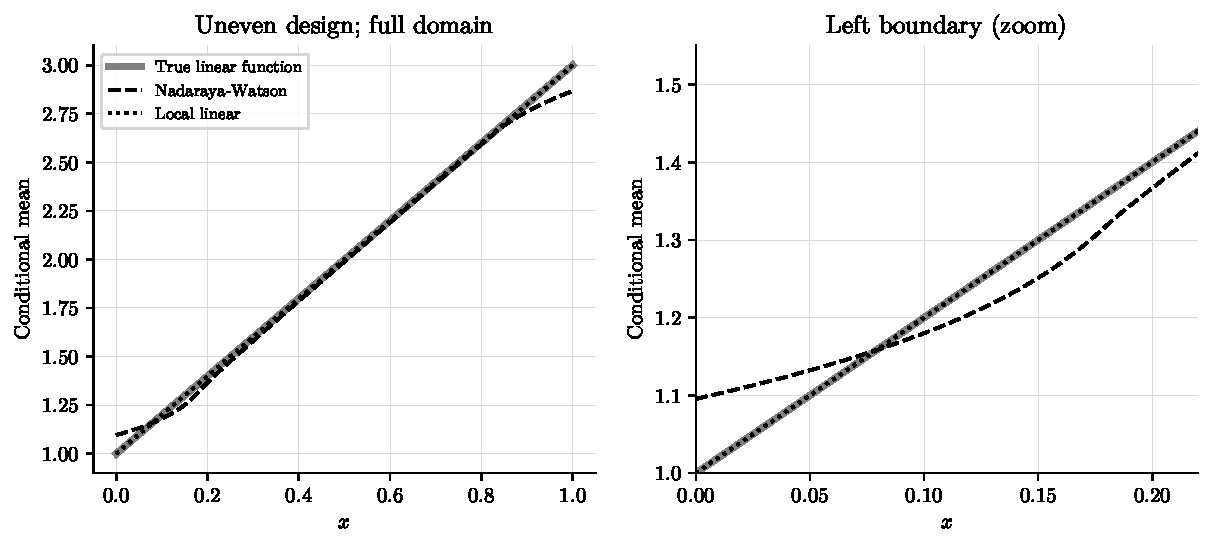
\includegraphics[width=.95\textwidth]{regression.pdf}
\caption{Làm trơn hàm tuyến tính trên các điểm thiết kế không đều,
$h=0.18$, kernel Epanechnikov. Đường vẽ dùng $Y_i=r(X_i)$ không có
nhiễu, nên biểu diễn kỳ vọng có điều kiện. Local linear tái tạo đường
thẳng; NW bị kéo bởi thiết kế và gần biên.}
\end{figure}
\intuition{Local linear dùng độ dốc như một tham số phụ để ước lượng
giá trị tại tâm chính xác hơn. Độ dốc không cần phải được báo cáo để
phương pháp tận dụng được nó.}

\section{Root--Unroot: từ số đếm đến hồi quy}
\subsection{Binning và xấp xỉ Poisson}
Giả sử mật độ trên $[0,1]$. Chia $k$ ô bằng nhau, trung điểm
$t_j=(j-1/2)/k$, số đếm $N_j$, xác suất ô $p_j$.
Nếu $f$ ít biến thiên trong ô,
$p_j\approx f(t_j)/k$ và $\lambda_j=np_j\approx nf(t_j)/k$.
Trong mô hình cố định $n$, $(N_1,\ldots,N_k)$ đa thức,
\[
\E N_j=np_j,\quad\Var N_j=np_j(1-p_j),\quad
\Cov(N_j,N_\ell)=-np_jp_\ell\quad(j\ne\ell).
\]
Các số đếm không độc lập. Với ô có xác suất nhỏ, từng số đếm có thể
xấp xỉ Poisson; trong mô hình Poisson hóa tổng số quan sát,
các số đếm độc lập Poisson thật sự.

\subsection{Lấy căn để ổn định phương sai}
Với $N\sim\operatorname{Poisson}(\lambda)$, xét $g(N)=\sqrt{N+c}$.
Delta method cho
\[
\Var g(N)\approx[g'(\lambda)]^2\lambda
=\frac{\lambda}{4(\lambda+c)}\approx\frac14
\]
khi $\lambda$ lớn. Taylor bậc hai cho kỳ vọng:
\begin{align*}
\E g(N)&\approx\sqrt{\lambda+c}
-\frac{\lambda}{8(\lambda+c)^{3/2}}\\
&=\sqrt\lambda+\frac{c/2-1/8}{\sqrt\lambda}
+\text{các hạng bậc nhỏ hơn}.
\end{align*}
Chọn $c=1/4$ triệt tiêu hiệu chỉnh bias dẫn đầu.
Đây là xấp xỉ, không phải kỳ vọng chính xác của căn số đếm.
Đặt
\[
\boxed{Y_j=\sqrt{\frac{k}{n}(N_j+1/4)}.}
\]
Khi xấp xỉ đủ tốt,
\[
Y_j\approx r(t_j)+\sigma\varepsilon_j,
\quad r(x)=\sqrt{f(x)},\quad \sigma^2\approx\frac{k}{4n},
\quad\varepsilon_j\text{ gần chuẩn tắc}.
\]
Ở ô rất ít số đếm, gần chuẩn có thể kém. Quy tắc $k\approx n/10$ trong
Wasserman là lựa chọn thực hành, không bảo đảm điều kiện tiệm cận hay
đếm đủ lớn ở mọi ô.

\subsection{Hồi quy, lấy phần dương và chuyển ngược}
Áp dụng hồi quy phi tham số cho $(t_j,Y_j)$ để có $\widehat r(x)$.
Đặt $r_+(x)=\max\{\widehat r(x),0\}$ và
\[
\boxed{\widehat f_{\rm RU}(x)=
\frac{r_+(x)^2}{\int_0^1r_+(t)^2\,dt}.}
\]
Phải kiểm tra mẫu số hữu hạn và dương. Nếu mẫu số bằng 0, quy trình
không trả được mật độ, cần xem lại hồi quy hoặc dữ liệu.
Lấy phần dương trước bình phương tránh biến một dự đoán âm của căn mật
độ thành mật độ lớn giả tạo. Chuẩn hóa đảm bảo tổng diện tích 1.

\begin{example}
$n=40$, $k=4$, số đếm $(4,8,12,16)$, nên
\[
Y_j^2=(N_j+1/4)/10=(0.425,0.825,1.225,1.625).
\]
$\sigma^2\approx0.025$, $\sigma\approx0.15811$.
Nếu \emph{chưa làm trơn} và giữ căn hằng theo từng ô, tích phân bình
phương là $(0.425+0.825+1.225+1.625)/4=1.025$.
Chiều cao chuẩn hóa là $(17,33,49,65)/41$.
Ví dụ chỉ kiểm tra biến đổi và chuẩn hóa; bước hồi quy thực sự vẫn cần
thiết lập bandwidth hoặc mức mô hình riêng.
\end{example}
\intuition{Binning tạo dữ liệu hồi quy; bước hồi quy mới quyết định độ
trơn cuối cùng. Lấy căn làm nhiễu ở các ô có mật độ khác nhau gần cùng
variance, rồi unroot đưa kết quả về mật độ.}
\source{\cite{wasserman}, Mục 6.6, trang in 139--140 (PDF 148--149)}

\section{Root--Unroot và băng tin cậy: mục tiêu nào được phủ?}
Trong mô hình Gaussian hồi quy lý tưởng, một smoother tuyến tính
$\widehat r(x)=\sum_j\ell_j(x)Y_j$ có kỳ vọng
$r_s(x)=\sum_j\ell_j(x)r(t_j)$ và variance
$\sigma^2\sum_j\ell_j(x)^2$ nếu các nhiễu độc lập.
Trên lưới $q$ điểm $x_1,\ldots,x_q$, khi $\sigma$ biết và mô hình đúng,
Bonferroni cho khoảng đồng thời của $r_s$ trên lưới:
\[
\widehat r(x_a)\pm z_{1-\alpha/(2q)}\sigma
\sqrt{\sum_j\ell_j(x_a)^2},\quad a=1,\ldots,q.
\]
Vì tổng xác suất thất bại ở $q$ điểm không quá $\alpha$, các khoảng
phủ đồng thời ít nhất $1-\alpha$. Đây chưa phải băng trên continuum;
mô hình Root--Unroot thật còn có sai số Poisson/Gaussian và binning.
Muốn phủ $r=\sqrt f$ thay vì $r_s$, phải xử lý bias hoặc undersmooth.

Giả sử đã có băng hợp lệ $L(x)\leq\sqrt{f(x)}\leq U(x)$ trên cả miền.
Vì hàm bình phương đơn điệu trên $[0,\infty)$,
\[
[\max\{L(x),0\}]^2\leq f(x)\leq[\max\{U(x),0\}]^2
\]
trên sự kiện phủ. Không tự chuẩn hóa hai đầu băng bằng cùng mẫu số
ngẫu nhiên của estimator: điều đó đổi đối tượng phủ và cần chứng minh
riêng. Chỉ bình phương khoảng cho $r_s$ cho khoảng của $r_s^2$, không
nhất thiết của mật độ thật $f$.
\intuition{Một biến đổi đẹp không xóa chệch làm trơn hay sự phụ thuộc của
số đếm. Cần báo rõ băng phủ hàm thật, hàm đã làm trơn, hay chỉ các giá trị
trên một lưới.}
\source{\cite{wasserman}, Mục 5.7, đặc biệt trang in 89--90 (PDF 99--100),
và Mục 6.6}

\section{KDE nhiều chiều và lời nguyền số chiều}
Với $X_i\in\R^d$, kernel tích chuẩn hóa và bandwidth chung $h$,
\[
\widehat f_h(x)=\frac1{nh^d}\sum_i
\prod_{a=1}^dK((x_a-X_{ia})/h).
\]
Đổi biến từng tọa độ cho $dx=h^ddu$, nên tích phân estimator bằng 1.
Với kernel đối xứng bậc hai, mật độ đủ trơn, miền không gây bias biên,
Taylor nhiều chiều cho
\[
\Bias(\widehat f_h(x))=
\frac{h^2\mu_2(K)}2\sum_{a=1}^d\partial_{aa}f(x)+o(h^2),
\quad
\Var\widehat f_h(x)\approx\frac{f(x)R(K)^d}{nh^d}.
\]
Hạng bậc một mất do moment một bằng 0. Hạng hỗn hợp
$u_au_b$ với $a\ne b$ mất vì tích hai moment một; hạng đường chéo
$u_a^2$ giữ lại, cho Laplacian $\sum_a\partial_{aa}f$.
Với phần dư tích phân kiểm soát được, AMISE có dạng
$Ah^4+B/(nh^d)$. Đạo hàm:
\[
4Ah^3-\frac{dB}{nh^{d+1}}=0
\quad\Longrightarrow\quad
\boxed{h_*\asymp n^{-1/(4+d)},\quad\MISE=O(n^{-4/(4+d)}).}
\]
Ở $d=1$, số mũ $4/5$; $d=6$, số mũ chỉ còn $2/5$.
Giả sử bỏ qua hằng số và muốn cùng quy mô sai số như $d=1$, cỡ mẫu
$n_1$, cần $n_d\approx n_1^{(d+4)/5}$.
Nếu $n_1=100$, thì $n_2\approx251$, $n_6\approx10\,000$,
$n_{10}\approx398\,107$. Đây chỉ là so sánh theo tốc độ, không phải
cỡ mẫu bảo đảm cho mọi mật độ.
\intuition{Thể tích cửa sổ giảm theo $h^d$, nên dữ liệu lân cận nhanh
chóng thưa khi tăng số chiều. Cấu trúc bổ sung như mô hình cộng hoặc
chiều nội tại thấp có thể giúp, nhưng thay đổi lớp bài toán và giả thiết.}
\source{\cite{wasserman}, Mục 6.5, trang in 138--139 (PDF 147--148)}

\chapter{Ngân hàng bài tập có lời giải từng bước}\label{ch:exercises}
Các bài dưới đây là bài luyện tự biên soạn hoặc diễn giải từ dạng bài
trong các nguồn ở thư mục môn học, không được gán số bài của sách hay
đề thi chính thức. Dùng cùng quy ước kernel và quantile trong giáo trình.
Làm tròn ở bước cuối; giữ phân số hoặc biểu thức chuẩn tắc càng lâu càng tốt.

\section{Dạng 1: tính KDE và đạo hàm}
\begin{exercise}[Mẫu gốc và điểm không khả vi]\label{ex:original}
Cho $X=(1,2,4,5)$, $x=3$, $h=2$. Tính $\widehat f_2(3)$,
$\widehat f_2'(3)$, $\widehat f_2''(3)$ với Epanechnikov, Uniform,
Triangular và Gaussian. Giải thích nếu đạo hàm không tồn tại.
\end{exercise}
\begin{solution}
\step{1. Chuẩn hóa khoảng cách và các mẫu số.}
$n=4$, $(u_1,u_2,u_3,u_4)=(1,1/2,-1/2,-1)$.
Các mẫu số cho mật độ, đạo hàm một và hai là
$nh=8$, $nh^2=16$, $nh^3=32$.
\begin{center}
\begin{tabular}{ccccc}
\toprule $u$ & Epanechnikov & Uniform & Triangular & Gaussian\\\midrule
$1$ & $0$ & $1/2$ & $0$ & $\varphi(1)$\\
$1/2$ & $9/16$ & $1/2$ & $1/2$ & $\varphi(1/2)$\\
$-1/2$ & $9/16$ & $1/2$ & $1/2$ & $\varphi(1/2)$\\
$-1$ & $0$ & $1/2$ & $0$ & $\varphi(1)$\\\bottomrule
\end{tabular}
\end{center}
\step{2. Cộng trọng số và chia cho $nh$.}
\[
\widehat f_{\rm E}(3)=\frac{18/16}{8}=\boxed{\frac9{64}},\quad
\widehat f_{\rm U}(3)=\frac{2}{8}=\boxed{\frac14},\quad
\widehat f_{\rm T}(3)=\frac1{8}=\boxed{\frac18}.
\]
Với Gaussian,
\[
\widehat f_{\rm G}(3)=\boxed{\frac{\varphi(1)+\varphi(1/2)}4}
\approx0.14850901.
\]
Uniform dùng đầu mút đóng; nếu dùng $|u|<1$, giá trị tại đúng 3 sẽ
là $1/8$. Giá trị giới hạn quanh 3 vẫn phải kiểm tra riêng.

\step{3. Gaussian: dùng trực tiếp công thức đạo hàm.}
$K'$ lẻ, nên các cặp đối xứng triệt tiêu và $\widehat f_{\rm G}'(3)=0$.
$K''(\pm1)=0$, $K''(\pm1/2)=-3\varphi(1/2)/4$, nên
\[
\widehat f_{\rm G}''(3)=\frac{-3\varphi(1/2)/2}{32}
=\boxed{-\frac{3\varphi(1/2)}{64}}\approx-0.01650306.
\]

\step{4. Epanechnikov: xét tổng ở $3+\delta$.}
Với $|\delta|$ đủ nhỏ, hai điểm 2 và 4 ở trong cửa sổ. Tổng kernel
của chúng bằng $9/8-3\delta^2/8$.
Nếu $\delta>0$, chỉ điểm 5 ở đầu ngoài đi vào cửa sổ, đóng góp
$3\delta/4-3\delta^2/16$; nếu $\delta<0$, điểm 1 đi vào, cho
$-3\delta/4-3\delta^2/16$. Ghép hai phía:
\[
\widehat f_{\rm E}(3+\delta)=\frac9{64}
+\frac3{32}|\delta|-\frac9{128}\delta^2.
\]
Thương sai phân từ trái tiến về $-3/32$, từ phải về $3/32$.
Vì hai giới hạn khác nhau,
$\boxed{\widehat f_{\rm E}'(3)\text{ không tồn tại}}$;
đạo hàm bậc hai cổ điển cũng không tồn tại.
Tính đối xứng của hàm không buộc đạo hàm tại tâm tồn tại: $|\delta|$
là phản ví dụ đơn giản.

\step{5. Triangular và Uniform: kiểm tra tương tự.}
Với Triangular, hai điểm nội cho tổng 1; một điểm ở ranh giới đi vào cho
$|\delta|/2$:
\[
\widehat f_{\rm T}(3+\delta)=\frac18+\frac1{16}|\delta|.
\]
Hai độ dốc là $-1/16$ và $1/16$, nên cả hai đạo hàm yêu cầu không tồn tại.
Với Uniform đóng, tại 3 có bốn điểm được đếm, nhưng với
$0<|\delta|$ đủ nhỏ chỉ còn ba điểm. Vì thế
\[
\lim_{\delta\to0,\,\delta\ne0}\widehat f_{\rm U}(3+\delta)=\frac3{16}
\ne\frac14=\widehat f_{\rm U}(3).
\]
Hàm không liên tục tại 3, nên không có đạo hàm một hoặc hai ở đó.
\pitfall{Không dùng giá trị $K''=-3/2$ của Epanechnikov ở điểm nối;
không bỏ các điểm $u=\pm1$ khi kiểm tra giới hạn. Giá trị mật độ tại
đầu mút và tính khả vi của tổng là hai câu hỏi khác nhau.}
\end{solution}

\begin{exercise}[Cùng mẫu, điểm khả vi]
Giữ $X=(1,2,4,5)$ và $x=3$, đổi $h=3/2$. Tính ba đại lượng trên
cho cùng bốn kernel.
\end{exercise}
\begin{solution}
\step{1. Xác định điểm nội và ngoại.}
$u=(4/3,2/3,-2/3,-4/3)$. Với các kernel compact, hai điểm ngoài
không đóng góp, hai điểm còn lại không ở điểm nối hoặc ở 0.
Các mẫu số là $nh=6$, $nh^2=9$, $nh^3=27/2$.

\step{2. Epanechnikov.}
$K(\pm2/3)=\frac34(1-4/9)=5/12$, nên
\[
\widehat f(3)=\frac{2(5/12)}6=\boxed{\frac5{36}},\quad
\widehat f'(3)=\frac{-1+1}{9}=\boxed0,\quad
\widehat f''(3)=\frac{-3}{27/2}=\boxed{-\frac29}.
\]

\step{3. Uniform và Triangular.}
Uniform cho $\widehat f(3)=2(1/2)/6=\boxed{1/6}$,
hai đạo hàm bằng 0 vì estimator hằng trong một lân cận của 3.
Triangular cho $\widehat f(3)=2(1/3)/6=\boxed{1/9}$,
đạo hàm một bằng $(-1+1)/9=0$, đạo hàm hai bằng 0 tại điểm này.

\step{4. Gaussian.}
Đặt $a=\varphi(4/3)$, $b=\varphi(2/3)$:
\[
\widehat f(3)=\boxed{\frac{a+b}{3}}\approx0.16115269,\quad
\widehat f'(3)=\boxed0,
\]
\[
\widehat f''(3)=\frac{2[(7/9)a-(5/9)b]}{27/2}
=\boxed{\frac{4(7a-5b)}{243}}\approx-0.00739374.
\]
Ở đây áp dụng công thức đạo hàm hợp lệ vì tất cả đối số tránh điểm
không khả vi. Đây không phải chứng cứ rằng Uniform ước lượng $f''$ tốt:
đạo hàm bằng 0 chỉ phản ánh hàm hằng từng đoạn.
\end{solution}

\begin{exercise}[Biweight ở một điểm nội]
Cho $X=(0,1,2)$, $x=1$, $h=2$, kernel Biweight.
Tính mật độ, đạo hàm một và hai.
\end{exercise}
\begin{solution}
\step{1. Lập bảng ba giá trị.}
$u=(1/2,0,-1/2)$, mẫu số $(nh,nh^2,nh^3)=(6,12,24)$.
\[
K(\pm1/2)=\frac{15}{16}\left(\frac34\right)^2=\frac{135}{256},
\qquad K(0)=\frac{15}{16}.
\]
\step{2. Mật độ.}
\[
\widehat f_2(1)=\frac{270/256+240/256}{6}
=\boxed{\frac{85}{256}}.
\]
\step{3. Đạo hàm.}
$K'$ lẻ nên tổng bằng 0. Với $K''(u)=15(3u^2-1)/4$,
\[
K''(\pm1/2)=-\frac{15}{16},\qquad K''(0)=-\frac{15}{4},
\]
\[
\boxed{\widehat f_2'(1)=0,\qquad
\widehat f_2''(1)=\frac{-15/16-15/4-15/16}{24}
=-\frac{15}{64}.}
\]
Độ cong âm thể hiện hình dạng lõm xuống của estimator tại tâm mẫu này.
\end{solution}

\section{Dạng 2: tích phân hằng số kernel}
\begin{exercise}[Uniform và Triangular]
Tính trực tiếp $\mu_2(K)$ và $R(K)$ của hai kernel.
\end{exercise}
\begin{solution}
\step{1. Uniform.}
Đối xứng cho
\[
\mu_2=2\int_0^1u^2\frac12du=[u^3/3]_0^1=\boxed{1/3},
\quad
R=2\int_0^1(1/2)^2du=\boxed{1/2}.
\]
\step{2. Triangular.}
Trên $[0,1]$, $K=1-u$, nên
\[
\mu_2=2\int_0^1(u^2-u^3)du
=2\left(\frac13-\frac14\right)=\boxed{1/6},
\]
\[
R=2\int_0^1(1-2u+u^2)du
=2\left(1-1+\frac13\right)=\boxed{2/3}.
\]
Không bỏ hệ số 2 khi chuyển tích phân kernel chẵn từ $[-1,1]$ sang $[0,1]$.
\end{solution}

\begin{exercise}[Epanechnikov]
Kiểm tra chuẩn hóa, rồi tính $\mu_2$ và $R$.
\end{exercise}
\begin{solution}
\step{1. Diện tích.}
$\int K=(3/2)\int_0^1(1-u^2)du=(3/2)(1-1/3)=1$.
\step{2. Moment bậc hai.}
\[
\mu_2=\frac32\int_0^1(u^2-u^4)du
=\frac32\left(\frac13-\frac15\right)=\boxed{\frac15}.
\]
\step{3. Bình phương kernel.}
Phải bình phương cả hệ số $3/4$:
\[
R=\frac98\int_0^1(1-2u^2+u^4)du
=\frac98\left(1-\frac23+\frac15\right)
=\frac98\frac8{15}=\boxed{\frac35}.
\]
Hai hằng số này đi vào AMISE theo cách khác nhau: $\mu_2$ bình phương
trong squared bias, $R$ tuyến tính trong variance.
\end{solution}

\begin{exercise}[Biweight]
Tính $\mu_2$ và $R$ bằng khai triển đa thức.
\end{exercise}
\begin{solution}
\step{1. Chuẩn hóa.}
\[
\int K=\frac{15}{8}\int_0^1(1-2u^2+u^4)du
=\frac{15}{8}\frac8{15}=1.
\]
\step{2. Moment bậc hai.}
\[
\mu_2=\frac{15}{8}\int_0^1(u^2-2u^4+u^6)du
=\frac{15}{8}\left(\frac13-\frac25+\frac17\right)
=\frac{15}{8}\frac8{105}=\boxed{\frac17}.
\]
\step{3. Bình phương.}
$(1-u^2)^4=1-4u^2+6u^4-4u^6+u^8$, nên
\begin{align*}
R&=\frac{225}{128}\left(1-\frac43+\frac65-\frac47+\frac19\right)\\
&=\frac{225}{128}\frac{128}{315}=\boxed{\frac57}.
\end{align*}
Giữ phân số tránh sai số khi các số hạng đa thức triệt tiêu mạnh.
\end{solution}

\section{Dạng 3: bandwidth và cross-validation}
\begin{exercise}[Bandwidth tham chiếu chuẩn]
Với $X=(1,2,4,5)$, tính bandwidth Gaussian normal-reference.
So sánh hệ số chính xác $(4/3)^{1/5}$ với hệ số làm tròn 1.06.
\end{exercise}
\begin{solution}
\step{1. Tính độ lệch chuẩn mẫu.}
$\overline X=3$, tổng bình phương độ lệch là 10.
\[
s^2=\frac{10}{4-1}=\frac{10}{3},\qquad s\approx1.82574186.
\]
\step{2. Tính thừa số cỡ mẫu.}
$4^{-1/5}\approx0.75785828$. Do đó
\[
\boxed{h_{\rm NR}=(4/3)^{1/5}\sqrt{10/3}\,4^{-1/5}
\approx1.46559887.}
\]
Dùng 1.06 cho $h\approx1.46667281$. Khác biệt là làm tròn hệ số,
không phải phương pháp khác.
\step{3. Nếu dùng scale bền vững.}
Theo quantile nghịch đảo EDF, $Q_{0.25}=1$, $Q_{0.75}=4$, nên
$\IQR=3$, $\IQR/1.34\approx2.23881>s$.
Vậy $a=\min(s,\IQR/1.34)=s$. Quy tắc hệ số $0.9$ cho
$0.9s4^{-1/5}\approx1.24528823$.
\pitfall{Dùng phương sai plug-in $2.5$ thay $s^2=10/3$ làm thay đổi đáp số.
Phải ghi rõ định nghĩa scale và quy ước quantile.}
\end{solution}

\begin{exercise}[Uniform LOOCV bằng phân số]
Cho $X=(0,1,2)$, kernel Uniform. Tính $\widehat J(h)$ với
$h=3/4,3/2$, rồi chọn trong hai ứng viên.
\end{exercise}
\begin{solution}
\step{1. Tính tích phân bằng độ dài giao.}
Mỗi cửa sổ dài $2h$, cao $1/(2nh)$. Hai cửa sổ cách tâm $d$ giao trên
đoạn dài $(2h-|d|)_+$. Do đó
\[
\int\widehat f_h^2=\frac1{4n^2h^2}\sum_{i,j}(2h-|X_i-X_j|)_+.
\]
Trong chín cặp có thứ tự: ba cặp khoảng cách 0, bốn cặp khoảng cách 1,
hai cặp khoảng cách 2.

\step{2. Bandwidth $h=3/4$.}
Tổng độ dài giao là $3(3/2)+4(1/2)=13/2$.
Tích phân bình phương bằng $(13/2)/(36\cdot9/16)=26/81$.
Không có quan sát khác trong khoảng cách $h$ của mỗi điểm, nên tổng
LOO bằng 0:
\[
\boxed{\widehat J(3/4)=26/81\approx0.32098765.}
\]

\step{3. Bandwidth $h=3/2$.}
Tổng độ dài giao là $3(3)+4(2)+2(1)=19$.
Tích phân bằng $19/(36\cdot9/4)=19/81$.
Số hàng xóm LOO lần lượt là $(1,2,1)$, nên các mật độ LOO bằng
$(1/6,1/3,1/6)$ và tổng bằng $2/3$.
\[
\boxed{\widehat J(3/2)=\frac{19}{81}-\frac23\frac23
=-\frac{17}{81}\approx-0.20987654.}
\]
Chọn $\boxed{h=3/2}$ trong hai ứng viên vì tiêu chuẩn nhỏ hơn.
\pitfall{LOO đếm khoảng cách $\leq h$, còn phần tích phân bình phương
phụ thuộc khoảng giao khi khoảng cách $<2h$. Các bài này tránh trường
hợp khoảng cách bằng đúng $h$, nên quy ước đầu mút không đổi điểm CV.}
\end{solution}

\begin{exercise}[Gaussian LOOCV bằng tổng đôi]
Cho $X=(0,1)$, Gaussian. Tính CV tại $h=1/2,1$.
\end{exercise}
\begin{solution}
\step{1. Dùng kernel tích chập.}
$C_K(v)=e^{-v^2/4}/(2\sqrt\pi)$. Có hai cặp đường chéo và hai cặp
ngoài đường chéo, nên
\[
\int\widehat f_h^2=\frac{2C_K(0)+2C_K(1/h)}{4h}
=\frac{1+e^{-1/(4h^2)}}{4\sqrt\pi h}.
\]
\step{2. Mật độ LOO.}
Sau khi bỏ một điểm chỉ còn một điểm; mỗi giá trị LOO bằng
$\varphi(1/h)/h$. Vì $2/n=1$, số hạng trừ là
$2\varphi(1/h)/h$. Do đó
\[
\boxed{\widehat J(h)=\frac{1+e^{-1/(4h^2)}}{4\sqrt\pi h}
-\frac{2\varphi(1/h)}h.}
\]
\step{3. Thế số.}
\begin{center}
\begin{tabular}{cccc}
\toprule $h$ & $\int\widehat f_h^2$ & Tổng LOO & $\widehat J(h)$\\\midrule
$1/2$ & $0.38587167$ & $0.21596387$ & $0.16990780$\\
$1$ & $0.25089522$ & $0.48394145$ & $-0.23304623$\\\bottomrule
\end{tabular}
\end{center}
Chọn $\boxed{h=1}$ trong hai ứng viên. Với mẫu rất nhỏ, quyết định chỉ
minh họa phép tính; không cho biết bandwidth tối ưu toàn bộ miền dương.
\end{solution}

\section{Dạng 4: kiểm định KS từng bước}
\begin{exercise}[{Mẫu trên $[0,1]$}]\label{ex:ksuniform}
Cho $X=(0.1,0.4,0.6,0.8)$, kiểm định $H_0:X\sim U[0,1]$.
Tính $D_n^+$, $D_n^-$, $D_n$. Dùng DKW mức 5\% để quyết định.
\end{exercise}
\begin{solution}
\step{1. Sắp xếp và tính CDF null.}
Mẫu đã sắp, $F_0(X_{(i)})=X_{(i)}$.
\begin{center}
\begin{tabular}{ccccc}
\toprule $i$ & $u_i$ & $i/4-u_i$ & $u_i-(i-1)/4$\\\midrule
1 & $0.10$ & $0.15$ & $0.10$\\
2 & $0.40$ & $0.10$ & $0.15$\\
3 & $0.60$ & $0.15$ & $0.10$\\
4 & $0.80$ & $0.20$ & $0.05$\\\bottomrule
\end{tabular}
\end{center}
\step{2. Lấy cực đại của hai cột sai khác.}
\[
\boxed{D_4^+=0.20,\quad D_4^-=0.15,\quad D_4=0.20.}
\]
\step{3. So với ngưỡng bảo thủ hữu hạn mẫu.}
$\epsilon_4=\sqrt{\log40/8}\approx0.67905$.
$0.20<0.67905$, nên không bác bỏ bằng kiểm định DKW này.
Ngưỡng lớn phản ánh mẫu chỉ có bốn quan sát; không thể kết luận phân
phối đều đúng vì không bác bỏ.

\step{4. Kiểm tra thêm CvM và AD trên cùng mẫu.}
Các tâm so sánh CvM lần lượt là
\[
(0.125,0.375,0.625,0.875).
\]
\[
W_4^2=\frac1{48}+(-.025)^2+(.025)^2+(-.025)^2+(-.075)^2
=\boxed{\frac{17}{600}\approx0.02833333}.
\]
AD dùng công thức log ở Chương 1 cho
$\boxed{A_4^2\approx0.20438803}$.
Các số này là thống kê; cần phân phối null tương ứng để đưa ra quyết định
CvM hoặc AD, không so chúng với ngưỡng KS.
\end{solution}

\begin{exercise}[Null mũ được chỉ định đầy đủ]
Cho $X=(0.2,0.5,1,1.5)$, kiểm định với $F_0(x)=1-e^{-x}$,
$x\geq0$, tức tốc độ mũ cố định bằng 1. Tính KS.
\end{exercise}
\begin{solution}
\step{1. Tính $u_i$.}
\begin{center}
\begin{tabular}{ccccc}
\toprule $i$ & $X_{(i)}$ & $u_i$ & $i/4-u_i$ & $u_i-(i-1)/4$\\\midrule
1 & $0.2$ & $.18126925$ & $.06873075$ & $.18126925$\\
2 & $0.5$ & $.39346934$ & $.10653066$ & $.14346934$\\
3 & $1.0$ & $.63212056$ & $.11787944$ & $.13212056$\\
4 & $1.5$ & $.77686984$ & $.22313016$ & $.02686984$\\\bottomrule
\end{tabular}
\end{center}
\step{2. Cực đại hai phía.}
\[
\boxed{D_4^+=e^{-1.5}\approx0.22313016,\quad
D_4^-=1-e^{-0.2}\approx0.18126925,\quad D_4\approx0.22313016.}
\]
Nếu dùng DKW 5\%, không bác bỏ vì nhỏ hơn $0.67905$.
Không thay tốc độ bằng $1/\overline X$ trong bài này: đề đã chỉ định
tốc độ 1. Nếu fit tốc độ từ mẫu, cần phân phối null được hiệu chỉnh.
\end{solution}

\begin{exercise}[Dữ liệu trùng và giới hạn trái]
Cho $X=(0.2,0.2,0.7,0.9)$, null đều trên $[0,1]$.
Tính KS và giải thích cách xử lý bước nhảy cao $2/4$.
\end{exercise}
\begin{solution}
\step{1. Viết hai cột với tất cả thứ tự thống kê.}
Các $u_i=(.2,.2,.7,.9)$.
\[
\left(\frac i4-u_i\right)=(.05,.30,.05,.10),
\quad
\left(u_i-\frac{i-1}4\right)=(.20,-.05,.20,.15).
\]
Các giá trị ở thứ hạng giữa một nhóm trùng không tương ứng EDF thực
ở một khoảng riêng, nhưng cực đại đúng vẫn được giữ: dùng thứ hạng
cuối nhóm cho phía phải, thứ hạng đầu nhóm cho giới hạn trái.
\step{2. Kiểm tra tại giá trị khác nhau.}
Tại $x=.2$, $\Fhat(.2)=.5$, $\Fhat(.2-)=0$.
Sai khác bên phải là $.5-.2=.3$, bên trái là $.2-0=.2$.
Tại $.7$, hai sai khác là $.75-.7=.05$ và $.7-.5=.2$;
tại $.9$, là $.1$ và $.15$. Vậy
\[
\boxed{D_4^+=.3,\quad D_4^-=.2,\quad D_4=.3.}
\]
Nếu dữ liệu trùng do làm tròn hoặc do phân phối rời rạc, mô hình quan
sát cần được xét lại khi hiệu chỉnh mức kiểm định. Trong một mô hình
liên tục chính xác, xác suất có các giá trị trùng đúng bằng nhau là 0.
Phép tính thống kê vẫn xác định; diễn giải null phải phù hợp dữ liệu.
\end{solution}

\section{Bốn bài chứng minh củng cố}
\begin{exercise}[EDF, covariance và DKW]
Chứng minh covariance EDF khi $x<y$ bằng số đếm; tìm cỡ mẫu để băng
DKW 95\% có nửa độ rộng không quá $0.05$.
\end{exercise}
\begin{solution}
\step{1. Chia ba vùng loại trừ nhau.}
Đặt $A_i=\1_{X_i\leq x}$, $B_i=\1_{x<X_i\leq y}$.
Với $p=F(x)$, $q=F(y)$, $\E A_i=p$, $\E B_i=q-p$,
và $A_iB_i=0$. Vì thế
$\Cov(A_i,B_i)=-p(q-p)$.
\step{2. Dùng $\1_{X_i\leq y}=A_i+B_i$.}
\[
\Cov(A_i,A_i+B_i)=p(1-p)-p(q-p)=p(1-q).
\]
Giữa quan sát khác nhau, covariance bằng 0. Chia tổng covariance cho
$n^2$ cho $\boxed{p(1-q)/n}$.
\step{3. Giải điều kiện độ rộng.}
\[
\sqrt{\frac{\log40}{2n}}\leq.05
\iff n\geq\frac{\log40}{2(.05)^2}\approx737.77589.
\]
Lấy số nguyên lớn hơn hoặc bằng: $\boxed{n\geq738}$.
Không làm tròn xuống vì cần bảo đảm bất đẳng thức.
\end{solution}

\begin{exercise}[Histogram: MISE chính xác cho mật độ tuyến tính]
Cho $f(x)=2x$ trên $[0,1]$, $n=96$, $m=4$.
Tính squared bias tích phân và phương sai tích phân chính xác, rồi
so với AMISE.
\end{exercise}
\begin{solution}
\step{1. Xác suất từng ô.}
$h=1/4$ và
\[
p_j=\int_{(j-1)/4}^{j/4}2x\,dx
=\frac{j^2-(j-1)^2}{16}=\frac{2j-1}{16}.
\]
Vì thế $p=(1,3,5,7)/16$; kỳ vọng histogram ở ô $j$ là $p_j/h=(2j-1)/4$,
bằng $2c_j$. Bias tại $x$ là $2(c_j-x)$, chính xác vì mật độ tuyến tính.
\step{2. Squared bias tích phân.}
\[
\int b^2=\sum_{j=1}^4\int_{-h/2}^{h/2}4t^2dt
=4\frac{4h^3}{12}=\boxed{\frac1{48}}.
\]
\step{3. Phương sai tích phân.}
$\sum_jp_j^2=(1+9+25+49)/256=21/64$.
\[
\int\Var=\frac1{96/4}\left(1-\frac{21}{64}\right)
=\boxed{\frac{43}{1536}}.
\]
Tổng $\MISE=1/48+43/1536=\boxed{25/512\approx0.04882813}$.
\step{4. So với AMISE.}
$R(f')=4$ nên $h_*=(6/(4\cdot96))^{1/3}=1/4$.
AMISE tại đó là $4h^2/12+1/(nh)=1/48+1/24=\boxed{1/16}$.
AMISE khác MISE vì bỏ số hạng âm bậc $1/n$ trong variance tích phân.
\end{solution}

\begin{exercise}[AMISE và độ nhạy bandwidth]
Với Epanechnikov, $R(f'')=1$, $n=480$, tìm $h_*$, AMISE tối ưu và
AMISE tại $h_*/2$, $2h_*$; chứng minh tỷ số tổng quát.
\end{exercise}
\begin{solution}
\step{1. Thế các hằng số kernel.}
\[
\AMISE(h)=\frac{(1/5)^2}{4}h^4+\frac{3/5}{480h}
=\frac{h^4}{100}+\frac1{800h}.
\]
\step{2. Đạo hàm và nghiệm.}
$4h^3/100-1/(800h^2)=0\iff h^5=1/32$, nên
$\boxed{h_*=1/2}$. Khi đó squared bias bằng $1/1600$,
variance bằng $1/400$, tổng $\boxed{1/320}$.
\step{3. Hai ứng viên lệch tối ưu.}
\[
\AMISE(1/4)=\frac1{25600}+\frac1{200}
=\boxed{\frac{129}{25600}},\quad
\AMISE(1)=\frac1{100}+\frac1{800}=\boxed{\frac9{800}}.
\]
\step{4. Tỷ số tổng quát.}
Viết AMISE là $Ah^4+B/(nh)$. Tại nghiệm,
$B/(nh_*)=4Ah_*^4$. Vì vậy
\[
\boxed{\frac{\AMISE(ch_*)}{\AMISE(h_*)}
=\frac{c^4Ah_*^4+4Ah_*^4/c}{5Ah_*^4}
=\frac{c^4+4/c}{5}.}
\]
Đổi bandwidth nửa lần hoặc hai lần không gây thay đổi đối xứng về rủi ro,
vì bias bình phương tăng theo lũy thừa bốn.
\end{solution}

\begin{exercise}[Contrast, Pythagoras và tái tạo tuyến tính]
Chứng minh ba sự triệt tiêu sau: contrast có cực tiểu tại hệ số mẫu;
hạng chéo sai số chiếu bằng 0; local linear triệt tiêu thành phần độ dốc.
Nêu nguyên nhân khác nhau của mỗi sự triệt tiêu.
\end{exercise}
\begin{solution}
\step{1. Contrast.}
Với $g=\sum_{j\leq D}b_j\phi_j$,
\[
\gamma_n(g)=\sum_j(b_j^2-2b_j\widehat a_j)
=\sum_j(b_j-\widehat a_j)^2-\sum_j\widehat a_j^2.
\]
Tổng bình phương cực tiểu bằng 0 khi $b_j=\widehat a_j$.
Đó là hoàn thành bình phương, không phải một giả thiết độc lập.
\step{2. Pythagoras.}
$f-f_D$ có tích vô hướng 0 với mọi $\phi_j$, $j\leq D$;
$f_D-\widehat f_D$ là tổ hợp của các hàm này. Do tuyến tính,
$\inner{f-f_D}{f_D-\widehat f_D}=0$. Khi khai triển bình phương chuẩn,
hạng chéo mất do \emph{trực giao trong không gian hàm}.
\step{3. Local linear.}
Với $w_i=k_i(S_2-S_1d_i)/\Delta$,
\[
\sum_iw_id_i=\frac{S_2\sum_i k_id_i-S_1\sum_i k_id_i^2}{\Delta}
=\frac{S_2S_1-S_1S_2}{\Delta}=0.
\]
Taylor $r(X_i)=r(x)+r'(x)d_i+O(h^2)$;
$r'(x)\sum_iw_id_i=0$. Đây là \emph{đẳng thức moment của trọng số},
đúng với thiết kế cụ thể nếu $\Delta>0$.
\step{4. Kết luận.}
Ba thao tác cùng loại bỏ hạng nhưng lý do khác nhau: tối ưu đại số,
trực giao hàm, và ràng buộc moment. Không viết chung một câu
``do các biến độc lập'' cho cả ba.
\end{solution}

\section{Cách tự chấm bài}
Một lời giải đủ cần có định nghĩa estimator, bảng đối số hoặc ô, mẫu số
đúng, miền áp dụng, phép cộng/tích phân và kết luận.
Với đạo hàm, kiểm tra điểm nối trước khi tính.
Với bandwidth, ghi đây là tối ưu AMSE tại điểm, AMISE toàn cục hay CV
trên tập ứng viên. Với kiểm định, ghi null, thống kê, ngưỡng và quyết
định; tránh biến ``không bác bỏ'' thành ``chứng minh đúng''.

\appendix
\chapter{Bảng tra cứu, nguồn và tái lập}\label{app:reference}
\section{Các hằng số kernel}
Mọi kernel compact trong bảng dùng giá đỡ $[-1,1]$ và chuẩn hóa như
Chương 3. Với kernel Uniform có giá đỡ $[-1/2,1/2]$, các hằng số sẽ
khác; không trộn hai cách chuẩn hóa khi dùng cùng bandwidth.
\begin{center}
\begin{tabular}{lcc}
\toprule Kernel & $\mu_2(K)$ & $R(K)$\\\midrule
Gaussian & $1$ & $1/(2\sqrt\pi)$\\
Epanechnikov & $1/5$ & $3/5$\\
Uniform & $1/3$ & $1/2$\\
Triangular & $1/6$ & $2/3$\\
Biweight & $1/7$ & $5/7$\\
Triweight & $1/9$ & $350/429$\\
Tricube & $35/243$ & $175/247$\\\bottomrule
\end{tabular}
\end{center}
Các hằng số compact được kiểm chứng bằng tích phân đa thức chính xác
và tích phân số độc lập. Với Gaussian dùng tích phân chuẩn tắc.

\section{Bảng công thức và điều kiện tối thiểu cần nhớ}
\begin{longtable}{p{.20\textwidth}p{.72\textwidth}}
\toprule Chủ đề & Công thức và điều kiện\\\midrule\endhead
EDF & $\E\Fhat(x)=F(x)$, $\Var\Fhat(x)=F(x)(1-F(x))/n$;
mẫu i.i.d., không yêu cầu có mật độ.\\[4pt]
DKW & $\epsilon_n=\sqrt{\log(2/\alpha)/(2n)}$; băng cắt tại 0 và 1,
phủ đồng thời ít nhất $1-\alpha$.\\[4pt]
Plug-in & $T(\Fhat)$; nhất quán cần tính liên tục phù hợp hoặc LLN
và điều kiện moment của thống kê cụ thể.\\[4pt]
KS & $D_n=\max_i\{i/n-F_0(X_{(i)}),F_0(X_{(i)})-(i-1)/n\}$;
bảng null chuẩn dùng $F_0$ liên tục, đã chỉ định đầy đủ.\\[4pt]
Histogram & $N_j/(nh)$; bias thường $O(h)$, variance $O(1/(nh))$;
MISE $n^{-2/3}$ trong thiết lập trơn bậc một và phân hoạch thích hợp.\\[4pt]
KDE & $(nh)^{-1}\sum K((x-X_i)/h)$; $K\geq0$, $\int K=1$
đảm bảo mật độ.\\[4pt]
Bias KDE & $h^2\mu_2f''/2+O(h^4)$ dưới điều kiện đạo hàm bậc bốn
và moment tuyệt đối bậc bốn; không áp dụng ở biên chưa hiệu chỉnh.\\[4pt]
AMISE KDE & $h^4\mu_2^2R(f'')/4+R(K)/(nh)$;
cần điều kiện phần dư tích phân. $h_*\asymp n^{-1/5}$,
MISE $O(n^{-4/5})$.\\[4pt]
Normal reference & $(4/3)^{1/5}s n^{-1/5}$ với Gaussian và mật độ
tham chiếu chuẩn; scale bền vững hoặc hệ số $0.9$ cần ghi riêng.\\[4pt]
CV & $\int\widehat f_h^2-(2/n)\sum_i\widehat f_{(-i),h}(X_i)$;
giữ $h$, estimator LOO có mẫu số $n-1$.\\[4pt]
Phép chiếu & $\sum_{j\leq D}\widehat a_j\phi_j$;
rủi ro bằng sai số xấp xỉ cộng tổng variance hệ số. Không tự không âm.\\[4pt]
NW & $\sum k_iY_i/\sum k_i$; mẫu số dương, bias nội miền có
design bias $2r'f'/f$.\\[4pt]
Local linear & $(S_2T_0-S_1T_1)/(S_0S_2-S_1^2)$;
ma trận không suy biến, $\sum w_i=1$, $\sum w_i(X_i-x)=0$.\\[4pt]
Root--Unroot & $Y_j=\sqrt{(k/n)(N_j+1/4)}$;
variance gần $k/(4n)$ trong xấp xỉ Poisson đủ tốt;
hồi quy, lấy phần dương, bình phương và chuẩn hóa.\\[4pt]
Nhiều chiều & Với trơn bậc hai và xử lý biên phù hợp,
$h_*\asymp n^{-1/(4+d)}$, MISE $O(n^{-4/(4+d)})$.\\
\bottomrule
\end{longtable}

\section{Bản đồ nguồn để đọc sâu}
Số trang PDF tính từ 1 và có tính cả bìa; số trang in là số trong giáo
trình. Trong các slide, số slide trùng thứ tự trang PDF của các bản hiện có.
\begin{longtable}{p{.22\textwidth}p{.70\textwidth}}
\toprule Nội dung & Nguồn chính\\\midrule\endhead
EDF, plug-in, GOF & \cite{slide1}, 46 trang PDF; Wasserman Chương 2.
EDF/hội tụ đều ở slide 10--20; plug-in 30--35; GOF 36--46.\\[4pt]
Histogram & \cite{slide2}, slide 12--18; Wasserman Mục 6.2,
chứng minh MISE trong phụ lục trang in 140--142, PDF 149--151.\\[4pt]
KDE và bandwidth & \cite{slide2}, slide 19--29; Wasserman Mục 6.3,
trang in 132--136, PDF 141--145.\\[4pt]
Hölder và minimax & Tsybakov Mục 1.2, đặc biệt Mệnh đề 1.1--1.2
và Định lý 1.1, trang in 4--9, PDF 15--20;
Chương 2 cho công cụ lower bound.
Wasserman Định lý 6.31, trang in 134--135, PDF 143--144,
cho lower bound MISE trên lớp đạo hàm $L_2$.\\[4pt]
Phép chiếu & \cite{projection}, slide 8--24; \cite{slide2}, slide 30--34.
Tsybakov Mục 1.7 bổ sung nền chuỗi trực chuẩn; lưu ý phần đó chủ yếu
xét hồi quy, không thay nguyên xi variance hồi quy bằng variance mật độ.\\[4pt]
Hồi quy và băng & Wasserman Mục 5.4 về hồi quy cục bộ, Mục 5.7
về băng tin cậy; trang in 89--90, PDF 99--100, nêu vấn đề mục tiêu
làm trơn so với hàm thật. Tsybakov Mục 1.5--1.6.\\[4pt]
Root--Unroot & Wasserman Mục 6.6, trang in 139--140, PDF 148--149.\\[4pt]
KDE nhiều chiều & Wasserman Mục 6.5, trang in 138--139, PDF 147--148.\\
\bottomrule
\end{longtable}

\subsection{Các điểm được làm rõ khi đối chiếu}
\begin{enumerate}
\item Chệch histogram và KDE cần phân biệt giá trị tại điểm, toàn miền,
và tích phân. Không tích phân một chặn điểm hằng trên miền vô hạn.
\item Nhân $K_4=(3-u^2)\varphi/2$ là bậc bốn theo định nghĩa moment
của tài liệu; tên ``bậc ba'' trong một số quy ước chỉ đếm số moment
bị triệt tiêu. Công thức moment mới là căn cứ.
\item Hölder bậc lớn hơn 1 phải dùng đạo hàm; histogram không tự đạt
$D^{-2\beta}$ với mọi $\beta$ chỉ vì mật độ trơn.
\item Đồng nhất thức contrast dùng $-2\nu_n(g)$ với
$\nu_n=P_n-P$. Dấu được suy lại từ định nghĩa, không sao chép dấu cộng
trong phác thảo slide chiếu.
\item Chuyển mật độ từ $[0,1]$ về $[a,b]$ cần hệ số $1/(b-a)$;
$1/\sqrt{b-a}$ chỉ là hệ số chuẩn hóa cơ sở $L_2$.
\item Không gán một hằng số phạt phổ quát từ ví dụ mô phỏng cho một
định lý oracle. Phác thảo Chương 4 ghi tường minh bước tập trung được
viện dẫn.
\end{enumerate}

\section{Tái lập bản PDF và kiểm chứng}
Thư mục chứa \texttt{main.tex}, các chương trong \texttt{chapters/},
bảy hình PDF trong \texttt{figures/}, script \texttt{verify\_and\_figures.py}
và báo cáo \texttt{verification.json}.
Chạy tại thư mục tài liệu:
\begin{verbatim}
python3 verify_and_figures.py
latexmk -xelatex -interaction=nonstopmode -halt-on-error main.tex
\end{verbatim}
Python cần NumPy, SciPy, SymPy, Matplotlib. Trên môi trường workspace
hiện tại, interpreter có sẵn các thư viện là
\path{/opt/anaconda3/bin/python}; có thể thay \texttt{python3} bằng đường
dẫn đó. XeLaTeX dùng Latin Modern, \texttt{polyglossia} và các gói trong
preamble; không yêu cầu font thương mại hay font cài riêng từ hệ điều hành.
Lệnh \texttt{make check} chạy cả kiểm chứng số, biên dịch và kiểm tra cấu
trúc PDF bằng \texttt{check\_document.py}; bước cuối cần thêm PyMuPDF.
Nếu cần chọn interpreter, dùng
\texttt{make check PYTHON=/opt/anaconda3/bin/python}.

Script dùng seed cố định, kiểm tra moment bằng đại số và tích phân số,
kiểm tra công thức đạo hàm bên trong miền, giới hạn một phía ở bài gốc,
CV qua công thức và tích phân độc lập, KS qua thuật toán thư viện,
CvM/AD qua tích phân trực tiếp, và tái tạo tuyến tính ở cả hai biên.
Các phép kiểm số không thay thế chứng minh tiệm cận hoặc lower bound.
\intuition{Nguồn, quy ước và cách chạy là một phần của tính tái lập.
Nếu đáp số khác phần mềm, kiểm tra chuẩn hóa kernel, quantile, mẫu số
variance và quy ước đầu mút trước khi kết luận công thức sai.}

\begin{thebibliography}{9}
\addcontentsline{toc}{chapter}{Tài liệu tham khảo}
\bibitem{slide1} Slide môn học, \emph{TKPTS\_Chương 1}, 46 trang PDF.
\bibitem{slide2} Slide môn học, \emph{Chap2\_Density\_estimation (handout)}, 37 trang PDF.
\bibitem{projection} Slide môn học, \emph{Chap2\_Density\_Estimation\_Projection\_estimator-2}, 29 trang PDF.
\bibitem{wasserman} Larry Wasserman (2006), \emph{All of Nonparametric Statistics}, Springer.
\bibitem{tsybakov} Alexandre B. Tsybakov (2009), \emph{Introduction to Nonparametric Estimation}, Springer.
\bibitem{localex} Các bài tập và lời giải tại \texttt{../Exercise/}, đặc biệt
\path{Chuong1_ECDF_BaiTap}, \path{test_loi_giai_mo_rong},
\path{KDE_Exam_Complete_Solutions}. Đây là nguồn bài luyện phụ trợ;
mọi công thức dùng trong giáo trình được kiểm tra lại.
\end{thebibliography}
\end{document}
